\documentclass[11pt]{article}

\PassOptionsToPackage{table}{xcolor}
\usepackage[review]{acl}

\usepackage{times}
\usepackage{latexsym}
\usepackage[T1]{fontenc}
\usepackage[utf8]{inputenc}
\usepackage{microtype}
% \usepackage{inconsolata}  % optional per ACL template; not available in this TeX Live
\usepackage{graphicx}
\usepackage{booktabs}
\usepackage{multirow}
\usepackage{amsmath}
\usepackage{amssymb}
\usepackage{amsthm}
\usepackage{enumitem}
\usepackage{pifont}
\usepackage{soul}
\usepackage{tikz}
\usetikzlibrary{arrows.meta,positioning,shapes.geometric,fit,backgrounds,calc}

\title{OntoCoDec: Type-Constrained Information Extraction\\via Compiled Schema Constraints}

\author{Anonymous ACL submission}

\begin{document}
\maketitle

% === Abstract ===
\begin{abstract}
Large language models for information extraction generate structurally valid but ontologically invalid triples: entity types that violate the schema's domain/range constraints for the predicted relation.
These domain/range violations (DR) persist even after fine-tuning and cannot be resolved by grammar-constrained decoding, which lacks cross-field type awareness.
We present \textsc{OntoCoDec} (\textbf{Onto}logy-\textbf{Co}mpiled \textbf{Dec}oding), a two-layer constrained decoding framework that compiles IE ontologies into decoding-time constraints: a grammar layer enforces structural validity; a semantic layer dynamically enforces cross-field type constraints during generation.
The two layers interact non-additively: grammar-only reduces DR by 3\% and semantic-only by 24\%, yet their composition achieves 94\%.
Composed with LoRA fine-tuning across three model families and two relation extraction datasets (up to 96 relations), OntoCoDec reduces DR to $\leq$\,0.21\% with minimal F1 impact ($\pm$0.3\,pp), converting irrecoverable type errors into correctable cross-field inconsistencies; beam search ($k{=}4$) achieves near-zero violations at ${\sim}$1.5$\times$ unconstrained latency.
Validation on a 70B model shows the semantic layer's independent effectiveness grows from 24\% to 84\% DR reduction with scale\footnote{Code and data are available at \url{https://anonymous.4open.science/r/schema_semantic_constrained_ie-FE20/}.}.
\end{abstract}


% === §1 Introduction ===
% Section 1: Introduction (compressed, 669→~550 words)

\section{Introduction}
\label{sec:introduction}

Large language models (LLMs) are increasingly used for information extraction (IE)~\cite{li2023codeie,sainz2024gollie,wei2023zeroshot}, but when generating relation triples $(h, r, t)$, neither entity necessarily carries a type consistent with the ontology's domain/range constraints for $r$.
We call such outputs \emph{domain/range violations} (DR): structurally valid triples that are ontologically invalid.
Violations are pervasive (15--18\% of triples under zero-shot decoding and 0.5--2\% even after LoRA fine-tuning) and correlate with schema restrictiveness rather than model scale.
At competitive quality, even low residual violation rates compound across thousands of documents into systematic knowledge graph corruption, making reliable constraint enforcement necessary.

Existing approaches leave a fundamental gap.
Schema-informed prompting reduces violations by 62\% on SciERC but is per-relation unreliable (violations for \textsc{Evaluate-for} actually \emph{increase} by 5.8\,pp).
Grammar-constrained decoding~\cite{dong2025xgrammar,willard2023outlines,beurer-kellner2023lmql} ensures syntactic well-formedness but cannot encode cross-field semantic constraints.
Post-hoc filtering discards up to 74\% of predictions including true positives (Appendices~\ref{app:cross-model-zs},~\ref{app:posthoc-extended}).
Training-based approaches~\cite{sainz2024gollie,lu2022uie} internalize schema knowledge but provide only soft guidance without runtime enforcement.

We propose \textbf{OntoCoDec}, a framework that translates IE ontologies into composable layers of decoding-time constraints.
A decidability analysis of IE type constraints (\S\ref{sec:decidability}) yields a two-layer architecture: the \emph{grammar layer} compiles ontology constraints into context-free grammars (CFGs) via XGrammar (JSON structure, vocabulary membership); the \emph{semantic layer} enforces type constraints at runtime via dynamic logit masking over an entity registry.
OntoCoDec compiles constraints automatically from IE ontologies, requires no constraint-specific training, and is applicable to any autoregressive LM with logits access.
We validate across three model families, two relation extraction (RE) datasets (up to 96 relation types), and event extraction (EE; \S\ref{sec:wikievents}), with 70B-class supporting evidence (\S\ref{sec:70b-results}).
Composed with LoRA, greedy decoding reduces DR to near-zero ($\leq$\,0.21\%) at relation F1 (R-F1) 40--46\% ($\pm$0.3 percentage points, $+$10\% latency), with 97.6--100\% of removed triples confirmed as false positives; beam ($k{=}4$) achieves near-zero violations at ${\sim}$1.5$\times$ latency.
DR enforcement converts irrecoverable ontology violations into cross-field type inconsistencies (CF;\,$\leq$\,1.4\% under fine-tuning), a severity downgrade amenable to post-hoc resolution.

OntoCoDec is orthogonal and complementary to training-based schema-aware approaches such as GoLLIE~\cite{sainz2024gollie} and KnowCoder~\cite{knowcoder_acl2024}; it can be composed with any generative IE system to improve schema compliance without retraining.

Our contributions:
\begin{enumerate}[leftmargin=*,itemsep=2pt]
    \item A two-layer constrained decoding framework that reduces domain/range violations to near-zero ($\leq$\,0.21\%) without retraining or significant quality loss, showing that these type constraints require stateful enforcement beyond context-free grammars (Proposition~1; \S\ref{sec:decidability}).
    \item An empirical finding of non-additive layer interaction: grammar-only reduces DR by 3\% and semantic-only by 24\%, yet their composition achieves 94\%, because grammar-enforced vocabulary membership creates the clean input the semantic layer requires.
    \item Scale-dependent layer interaction: the semantic layer's independent DR reduction grows from 24\% (8B) to 84\% (70B; \S\ref{sec:70b-results}), because larger models better satisfy the vocabulary prerequisites that enable semantic enforcement. Beam $k{=}4$ achieves near-zero violations at 8B; event extraction on WikiEvents confirms cross-task generalization (\S\ref{sec:wikievents}).
\end{enumerate}


% === §2 Related Work ===
\section{Related Work}
\label{sec:related_work}

We provide a detailed survey in Appendix~\ref{app:related_work}; here we position OntoCoDec along three axes.

\paragraph{Constrained decoding.}
Grammar-constrained decoding restricts each token to a mask derived from a target grammar.
XGrammar~\cite{dong2025xgrammar}, Outlines~\cite{willard2023outlines}, SGLang~\cite{zheng2024sglang}, SynCode~\cite{ugare2024syncode}, and related systems~\cite{beurer-kellner2023lmql,park2024grammar,jsonschemabench2025} compile JSON Schemas into pushdown automata for structural enforcement, but are limited to context-free constraints and cannot enforce cross-field semantic rules that depend on previously generated field values.
PICARD~\cite{scholak2021picard} and \citet{pldi2025_type_constrained_codegen} compile type systems into prefix automata; KG-Trie~\cite{luo2025kgtrie} applies trie-based KG constraints for knowledge-to-text generation.
OntoCoDec fills this gap with a stateful semantic layer whose entity registry is populated dynamically during generation.

\paragraph{Schema-aware IE.}
GoLLIE~\cite{sainz2024gollie}, KnowCoder~\cite{knowcoder_acl2024}, and others~\cite{guidex2025,josifoski2022genie,paolini2021tanl,cabot2021rebel,wang2023instructuie,qi2024adelie,fei2022lasuie,lu2022uie,zhou2024universalner} encode ontology structure via training-time internalization, learning schema preferences but without runtime guarantees: violations persist at 0.5--2\% even after fine-tuning~\cite{wadhwa2023revisiting}.
OntoCoDec provides orthogonal runtime enforcement composable with these systems, including GoLLIE itself (Appendix~\ref{app:gollie-comparison}).

\paragraph{Constraint enforcement in IE.}
\citet{roth_yih_2004} and \citet{riedel2010modeling} formulated hard type constraints via integer linear programming (ILP); post-hoc validation~\cite{khorshidi2025odke,spires_2024,ontologx_2025} detects violations after generation but discards up to 74\% of predictions; grammar-only enforcement~\cite{geng2023gcd,boostcd2025} achieves only 3\% DR reduction (\S\ref{sec:constrained-baselines}).
EnriCo~\cite{zaratiana2024enrico} uses answer set programming (ASP); IterGen~\cite{ugare2025itergen} backtracks on violations; \citet{vukovic2024dialogue} combines ontology constraints with constrained chain-of-thought for dialogue RE.
These methods either operate post-hoc (discarding predictions) or require iterative refinement; OntoCoDec prevents violations during generation via forward-only stateful masking at $O(|V|)$ per step.


% === §3 Method ===
% Section 3 — Method (Draft)
% OntoCoDec: Type-Valid Information Extraction
% via Compiled Ontology Constraints

\section{Method}
\label{sec:method}

\begin{figure*}[t]
\centering
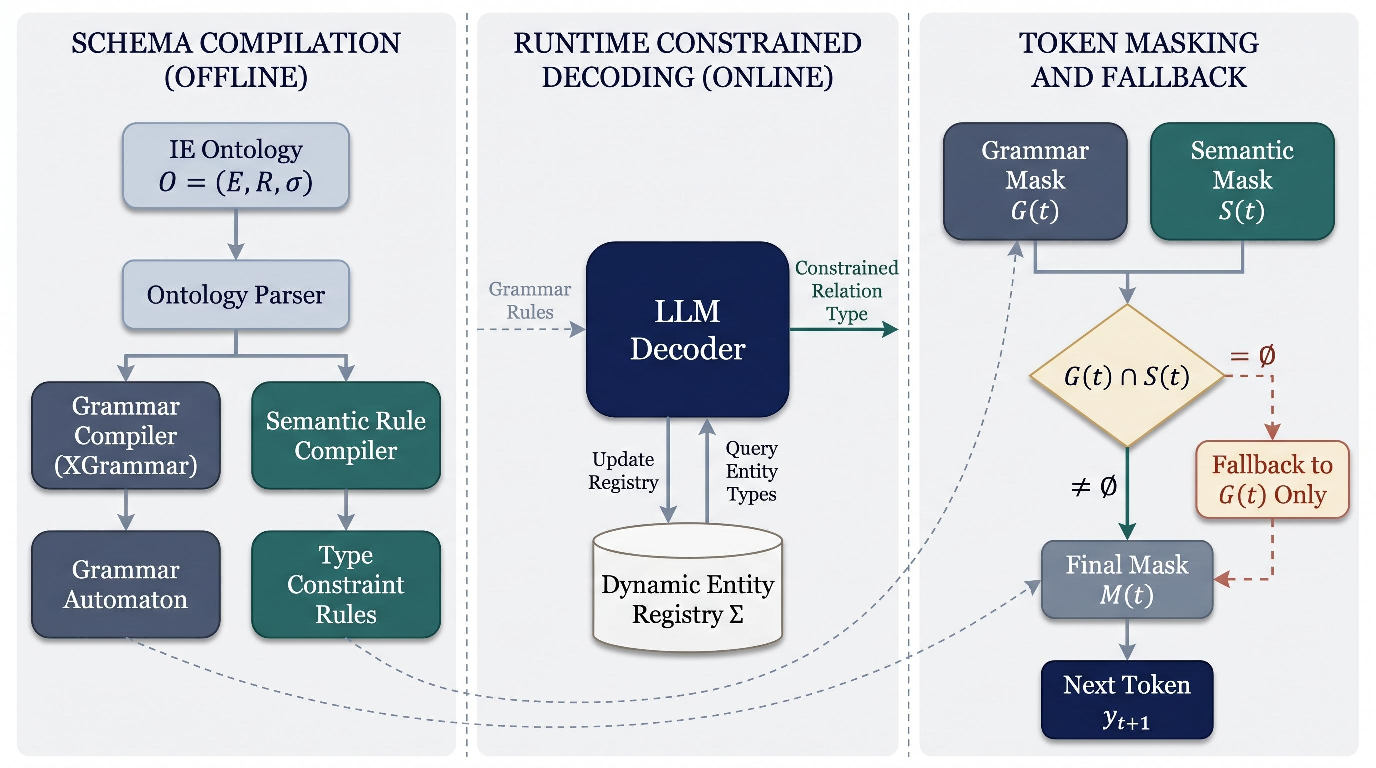
\includegraphics[width=\textwidth,height=6.5cm,keepaspectratio]{figures/fig1_framework.pdf}
\caption{Overview of OntoCoDec. An IE ontology is compiled into two constraint layers: a grammar layer (context-free) and a semantic layer (prefix-decidable with state). At each decoding step, the final mask $M_{\text{final}}(t) = G(t) \cap S(t)$ ensures both structural and type validity; when $S(t) \cap G(t) = \emptyset$, grammar-first fallback preserves JSON integrity.}
\label{fig:framework}
\end{figure*}


\paragraph{Preliminaries.}
\label{sec:preliminaries}
An IE ontology $\mathcal{O} = (\mathcal{E}, \mathcal{R}, \sigma)$ defines entity types $\mathcal{E}$, relation types $\mathcal{R}$, and a mapping $\sigma: \mathcal{R} \to \mathcal{P}(\mathcal{E} \times \mathcal{E})$ specifying valid (head type, tail type) pairs per relation.
A triple $(h, r, t)$ is \emph{type-valid} if $(\mathrm{type}(h), \mathrm{type}(t)) \in \sigma(r)$.
We quantify constraint restrictiveness via \emph{constraint tightness} $\kappa(r)$ (\S\ref{sec:composition}); empirical constraints achieve 99\%+ instance-level coverage (SciERC 99.0\%, DocRED 99.4\%), with grammar-first fallback (\S\ref{sec:composition}) ensuring no valid triples are blocked.
Given $\mathcal{O}$ and an autoregressive LM $\mathcal{M}$, we seek constraints $\mathcal{C}$ ensuring: (a)~\textbf{structural validity}, i.e., well-formed JSON with $\mathcal{E}$/$\mathcal{R}$ membership; and (b)~\textbf{type validity}, i.e., $(\mathrm{type}(h), \mathrm{type}(t)) \in \sigma(r)$ for every triple.
Condition (a) is context-free; (b) is context-sensitive but \emph{prefix-decidable}: at the point where a type token is generated, all information needed is available in the decoded prefix.

\smallskip
\noindent
We present OntoCoDec, a framework that translates IE ontologies into token-level constraints enforced during autoregressive generation.
The design is guided by a decidability analysis of IE type constraints.

\paragraph{Constraint decidability taxonomy.}
\label{sec:decidability}
We classify IE type constraints into three levels: (1)~\emph{context-free}: vocabulary membership and JSON structure; (2)~\emph{prefix-decidable with state}: domain/range type validity, determined at each type-bearing position given the decoded relation type and entity registry; (3)~\emph{non-local}: cross-entity type consistency, which depends on the full output.
Unlike code generation where types are statically declared, IE constraints fall into level~2: entity types are inferred from text, the registry is built dynamically, and constraint targets depend on the co-occurring relation.
OntoCoDec enforces levels 1--2 (grammar and semantic layers, respectively); level~3 is addressed by beam search or post-hoc resolution (Appendix~\ref{app:tcr}).

\smallskip
\noindent
Existing grammar-constrained decoding frameworks (e.g., XGrammar) enforce level~1 constraints (structural validity and vocabulary membership) but IE domain/range rules require cross-position entity-type state that context-free grammars cannot express.
Even when the entity set is finite, encoding type constraints into a deterministic finite automaton (DFA) requires $O(|\mathcal{E}|^{|\text{entities}|})$ states: for typical SciERC documents (median 17 entities, 6 types), $6^{17} \approx 1.6{\times}10^{13}$ states; for DocRED (median 19 entities, 6 types), $6^{19} \approx 6.1{\times}10^{14}$, well beyond practical construction for online decoding.
While cross-reference binding is known to exceed context-free expressiveness in programming language theory, its implications for IE-specific type constraints (where entity types are inferred from text rather than statically declared) have not been formally characterized.
Formally, domain/range constraints for unbounded entity sets are not context-free (\textbf{Proposition~1}; proof via pumping argument in Appendix~\ref{app:pumping-lemma}): a pushdown automaton (PDA) cannot retrieve the type of entity $e_k$ without destroying stack entries above it.
OntoCoDec's semantic layer addresses this with a runtime entity registry $\mathcal{D}$ (a finite map enabling random-access type lookups), avoiding both the theoretical impossibility (unbounded) and the engineering intractability (finite but exponential).

\noindent\textbf{Empirical Observation} (scale-dependent enabling dependency)\textbf{.} The grammar layer alone cannot enforce domain/range constraints (Proposition~1), while the semantic layer alone achieves only 24\% DR reduction at 8B without grammar-enforced vocabulary membership (\S\ref{sec:scierc-results}, Table~\ref{tab:scierc-ablation}).
The strength of this dependency is scale-dependent: at 70B, the semantic layer independently achieves 84\% DR reduction (\S\ref{sec:70b-results}), whereas 8B models show only 24\% independent reduction.
\smallskip

We describe the problem formulation (\S\ref{sec:formulation}), each layer, and two decoding strategies (\S\ref{sec:strategies}); formal analysis of constraint composition is in Section~\ref{sec:composition}.


\subsection{Problem Formulation}
\label{sec:formulation}

\paragraph{IE as structured generation.}
Given an input text $x$, a language model generates a structured JSON output $y$:
%
\begin{equation}\label{eq:output-schema}
\resizebox{.88\columnwidth}{!}{$\displaystyle
  y = \bigl\{\texttt{entities}: [\{n_i, \tau_i\}],\; \texttt{relations}: [\{h_j, t_j, r_j, \tau^h_j, \tau^t_j\}]\bigr\}
$}
\end{equation}
%
where each entity has a name $n_i$ and type $\tau_i \in \mathcal{E}$, and each relation specifies head $h_j$, tail $t_j$, relation type $r_j \in \mathcal{R}$, and head/tail entity types $\tau^h_j, \tau^t_j$.
The output JSON Schema (\S\ref{sec:grammar}) enforces a fixed field ordering (head $\to$ tail $\to$ relation $\to$ head\_type $\to$ tail\_type) via deterministic grammar compilation, ensuring the relation type $r_j$ is known before entity type fields and enabling sequential domain/range lookups (\S\ref{sec:dynamic-masking}).
The grammar structurally enforces entity-before-relation ordering (maintained in all documents across all configurations), ensuring the entity registry (\S\ref{sec:entity-registry}) is populated before relation-level type constraints are evaluated; unregistered entities trigger domain-only filtering.

\paragraph{Ontology compliance.}
Using the ontology $\mathcal{O} = (\mathcal{E}, \mathcal{R}, \sigma)$ defined above, we write $\operatorname{dom}(r) = \{\tau^h : \exists \tau^t,\, (\tau^h, \tau^t) \in \sigma(r)\}$ for domain-valid head types and $\operatorname{range}(r, \tau^h) = \{\tau^t : (\tau^h, \tau^t) \in \sigma(r)\}$ for the conditional range given head type $\tau^h$.
Our enforcement target is \emph{pair-based} type validity: $(\tau^h, \tau^t) \in \sigma(r)$ for every triple.
The decoder enforces this sequentially: $\tau^h \in \operatorname{dom}(r)$ at head position, then $\tau^t \in \operatorname{range}(r, \tau^h)$ at tail position, achieving best-effort pair-based enforcement (pair validity ensured when no fallback is triggered; domain-only filtering otherwise) strictly stronger than independent domain/range checks (which over-permit 33--37\% spurious pairs on SciERC/DocRED; \S\ref{sec:rectangularity}).


\subsection{Grammar Layer}
\label{sec:grammar}

A JSON Schema encoding Eq.~\eqref{eq:output-schema} with \texttt{enum} constraints ($\mathcal{E}$, $\mathcal{R}$) is compiled into a pushdown automaton via XGrammar~\cite{dong2025xgrammar}.
At step $t$, grammar-valid tokens $G(t) \subseteq V$ pass; all others receive logits $-\infty$, enforcing structural validity, vocabulary membership ($r_j \in \mathcal{R}$, $\tau_i \in \mathcal{E}$), but not domain/range constraints (which depend on entity types within each triple).

\subsection{Semantic Layer}
\label{sec:semantic}

The semantic layer enforces domain/range constraints through a stateful logits processor maintaining an entity registry during generation.
\emph{Running example}: for \textsc{Used-for} ($\operatorname{dom}{=}\{\textrm{Method}\}$, $\operatorname{range}{=}\{\textrm{Task}\}$), entity ``ResNet'' (Method) passes the head-type check while Material is blocked; ``image classification'' (Task) passes the tail-type check.

\paragraph{Entity registry.}
\label{sec:entity-registry}
The semantic layer builds a registry $\mathcal{D}: \text{name} \to \text{type}$ incrementally during entity generation: each completed entry $\{n_i, \tau_i\}$ adds $(n_i, \tau_i)$ to $\mathcal{D}$, which is consulted during relation generation for type lookups.
The registry uses \emph{first-seen} semantics: when an entity name appears in multiple triples, the type assigned at its first occurrence governs all subsequent constraint checks, making type enforcement sensitive to generation order.
At each step $t$, the processor pattern-matches the decoded prefix to identify the current field position; semantic masks activate only at type-bearing positions (\textsc{HeadType}, \textsc{TailType}).
\label{sec:position-detection}

\paragraph{Dynamic masking.}
\label{sec:dynamic-masking}
At type-bearing positions, the processor computes a semantic mask $S(t) \subseteq V$.
At a \textsc{HeadType} position, if $h_j \in \mathcal{D}$ and $\mathcal{D}[h_j] \in \operatorname{dom}(r_j)$, the mask allows only the registered type; otherwise it falls back to all domain-valid types $\operatorname{dom}(r_j)$.
At a \textsc{TailType} position, the mask restricts to $\operatorname{range}(r_j, \tau^h_j)$ conditioned on the already-determined head type, further narrowing to the registered type when $t_j \in \mathcal{D}$.
This sequential check achieves best-effort pair-based enforcement (\S\ref{sec:formulation}), strictly tighter than independent domain/range checking; ``best-effort'' reflects the grammar-first fallback (\S\ref{sec:composition}), which prioritizes JSON integrity over type validity when constraints conflict.

\paragraph{Tokenizer-agnostic type masking.}
We use \emph{continuation masking} to handle context-dependent tokenizations and prefix-shared types (e.g., \textsc{Sen}/\textsc{Sid}/\textsc{Side} in WikiEvents): a compile-time prefix map identifies valid continuations for each type name, disambiguating over multiple steps across byte-level byte pair encoding (BPE) (Qwen, Llama) and SentencePiece (Mistral).

\paragraph{Grammar-semantic interaction.}
\label{sec:interaction}
The final mask is $G(t) \cap S(t)$; when empty, grammar-first fallback applies (\S\ref{sec:composition}), embodying this interaction: semantic constraints reduce DR by only 24\% without grammar-enforced vocabulary.


\subsection{Decoding Strategies}
\label{sec:strategies}

\paragraph{S1 (joint extraction): Single-pass decoding.}
Both layers are active throughout generation; the entity registry populates during entity decoding and is immediately available for relation-level type checking.

\paragraph{S2 (two-pass pipeline): Two-pass decoding.}\label{sec:s2}
A first pass extracts entities; these compile an input-dependent grammar for the second pass.
S1 achieves higher R-F1 at comparable DR (\S\ref{sec:scierc-results}) and is the primary configuration.


% === §5 Constraint Composition ===
\section{Constraint Composition}
\label{sec:composition}
% Section: Constraint Composition (compressed, 787→~500 words)

% ──────────────────────────────────────────
%  Figure: Composition Interaction
% ──────────────────────────────────────────
\begin{figure}[t]
\centering
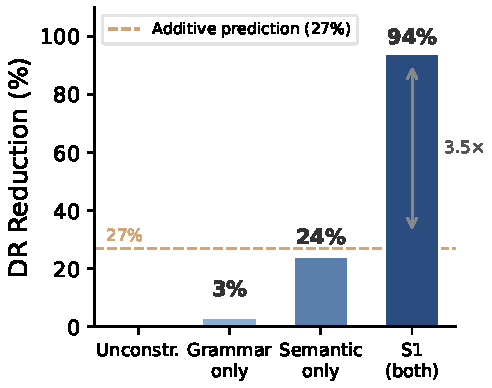
\includegraphics[width=\columnwidth]{figures/fig_composition_interaction.pdf}
\caption{Non-additive layer interaction on SciERC (Qwen3-8B, zero-shot). Grammar-only and semantic-only achieve 3\% and 24\% DR reduction; their composition yields 94\%, 3.5$\times$ the additive prediction.}
\label{fig:composition-interaction}
\end{figure}

At each decoding step $t$, let $G(t) \subseteq V$ and $S(t) \subseteq V$ denote the tokens permitted by the grammar and semantic layers, respectively.
The final mask is their conjunction:
%
\begin{equation}\label{eq:composition}
  M_{\text{final}}(t) = M_{\text{grammar}}(t) \;\wedge\; M_{\text{semantic}}(t),
\end{equation}
%
where $\wedge$ denotes element-wise AND over the vocabulary $V$; a token is allowed only if it satisfies \emph{both} structural and type-level constraints.
The conjunction is asymmetric: $S(t)$ is defined only over $G(t)$. This reflects the scale-dependent layer interaction (\S\ref{sec:method}): the semantic layer requires the relation type to belong to $\mathcal{R}$, a property enforced only by the grammar layer.
This dependency is scale-sensitive: 70B semantic-only achieves 84\% DR reduction (vs.\ 24\% on 8B), though grammar remains necessary for RV elimination (\S\ref{sec:70b-results}).

\paragraph{Grammar-First Fallback.}
When $S(t) \cap G(t) = \emptyset$ (tight constraints leave no token that is both grammar-valid and semantically valid), na\"{\i}ve masking would force selection of a grammar-invalid token, breaking JSON structure.
We enforce a \emph{grammar-first fallback}: semantic masking is skipped and the grammar layer alone controls selection.
Structural integrity is a hard constraint; type violations are soft errors detectable by downstream validation, with DR (ontologically invalid type pair) more severe than CF (individually valid triples with cross-triple type inconsistency).
Extraction tasks are robust to format-level constraints~\cite{tam2024letmespeak}, supporting this asymmetric treatment.

\paragraph{Constraint Tightness.}
\label{eq:tightness}
Per-relation constraint tightness $\kappa(r) = 1 - |\sigma(r)|/|\mathcal{E}|^2$ captures schema restrictiveness; DR reduction correlates descriptively with schema-mean $\bar{\kappa}$ across our three evaluation schemas ($n{=}3$), though entity type confusability is a significant co-factor (Appendices~\ref{app:kappa-case-study},~\ref{app:kappa-analysis},~\ref{app:tcr}).
Figure~\ref{fig:dual-factor-scatter} shows that residual DR is governed by the product $\bar{\kappa} \times \text{RV}_{\text{baseline}}$ for calibrated models ($R^2{=}0.886$, $n{=}4$; descriptive only).

% ──────────────────────────────────────────
%  Figure: Dual-Factor Scatter (moved from appendix)
% ──────────────────────────────────────────
\begin{figure}[t]
\centering
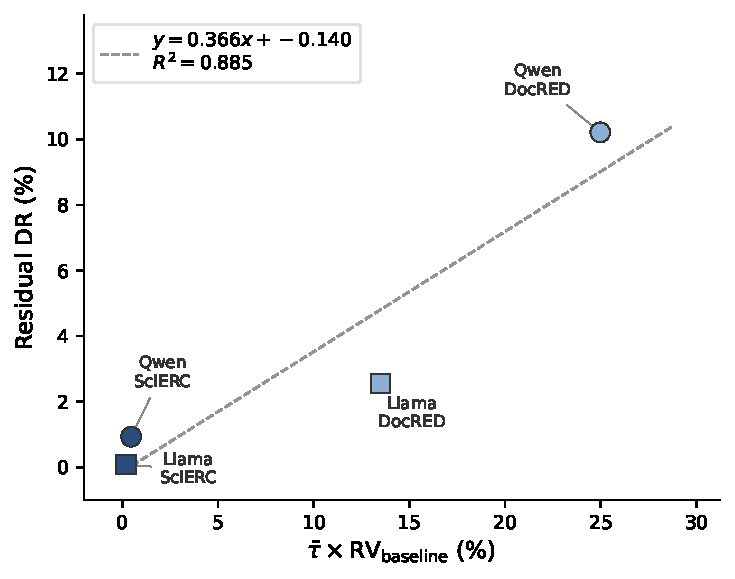
\includegraphics[width=\columnwidth]{figures/dual_factor_scatter.pdf}
\caption{Residual DR vs.\ $\bar{\kappa} \times \text{RV}_{\text{baseline}}$ across model$\times$dataset configurations. Linear fit (calibrated models): $R^2{=}0.886$ ($n{=}4$, $p{=}0.058$; descriptive only).}
\label{fig:dual-factor-scatter}
\end{figure}

\paragraph{Greedy limitation and fallback cascade.}
\label{sec:greedy-limitation}
Single-pass per-triple enforcement cannot coordinate type assignments across triples sharing the same entity mention; cross-field consistency requires global inference that exceeds the per-token masking paradigm.
The semantic layer commits entity types greedily, an instance of Level~3 (non-local) constraints (\S\ref{sec:decidability}), so CF violations arise when the same entity receives different types across triples; beam search mitigates this (\S\ref{sec:beam-results}).
Fallback triggers on 0.5--5.7\% of type-bearing positions (zero-shot), virtually eliminated by fine-tuning ($\leq$\,0.11\%); all residual DR occurs at fallback positions (Appendices~\ref{app:causal-tracing},~\ref{app:fallback-coverage}).

\paragraph{Non-rectangularity and independent enforcement.}
\label{sec:rectangularity}
Type signatures are non-rectangular (0/7 SciERC, 23/96 DocRED rectangular); independent enforcement admits 33--37\% spurious pairs, eliminated by fine-tuning (Table~\ref{tab:composability}).
Shuffling type order produces byte-identical outputs across all 551 SciERC documents, confirming order invariance (Appendix~\ref{app:order-invariance}).



% === §6 Experiments ===
\section{Experiments}
\label{sec:experiments}

% §5 Setup (compressed from Violation Landscape)

\label{sec:violation_landscape}

We evaluate OntoCoDec in two deployment configurations: greedy S1 (DR\,$\leq$\,0.21\%, $+$10\% latency) and beam S1 (near-zero violations, 1.39$\times$ latency); zero-shot evaluation (\S\ref{sec:scierc-results}; Appendix~\ref{app:cross-model-zs}) serves as a diagnostic probe for the fine-tuned setting (relation F1 (R-F1) 40--46\%).

\paragraph{Setup.}
We evaluate on SciERC~\cite{luan2018scierc} (551 test sentences, 7 relations, $\bar{\kappa}{=}0.333$) and DocRED~\cite{yao2019docred} (998 development documents; test annotations are not publicly available; 96 relations, $\bar{\kappa}{=}0.842$).
RE type constraints are extracted from observed type pairs in training data (neither dataset provides a standalone ontology specification); EE constraints on WikiEvents (\S\ref{sec:wikievents}) derive from the KAIROS ontology.
All constraints are schema-level, independent of evaluation splits.
Primary model: Qwen3-8B~\cite{qwen2025qwen3}, zero-shot greedy decoding; cross-model validation in Appendix~\ref{app:cross-model-zs}, composability with fine-tuning in \S\ref{sec:composability}.
LoRA hyperparameters (rank, $\alpha$, learning rate) were tuned on SciERC and transferred to DocRED without dataset-specific optimization; given the substantial schema complexity difference (7 vs.\ 96 relations), this transfer may underestimate DocRED fine-tuning potential.
Our R-F1 range (40--46\% under LoRA) is consistent with recent LLM-based generative RE evaluations on these benchmarks, where document-level closed IE without gold entity spans typically achieves 35--50\%~\cite{wadhwa2023revisiting}; supervised span-based methods operating under different assumptions (gold entity spans, dedicated architectures) are not directly comparable.
For reference, the supervised end-to-end SOTA on SciERC achieves 41.6\% strict Rel-F1 (PL-Marker~\cite{ye2022packed}) and 36.8\% (PURE~\cite{zhong2021frustratingly}); while evaluation protocols differ, our 40--46\% R-F1 range under LoRA falls within a comparable band.
DocRED development documents were used for evaluation only.
Prompt templates and reproducibility details (hyperparameters, dataset statistics) in Appendices~\ref{app:prompts} and~\ref{app:reproducibility}.
Four violation categories: \textbf{DR} (type pair $\notin \sigma(r)$), \textbf{RV} (relation $\notin \mathcal{R}$), \textbf{ET} (entity type $\notin \mathcal{E}$), \textbf{CF} (conflicting types across triples).
Baseline DR: 15.37\% (SciERC), 18.46\% (DocRED); schema-informed prompting reduces DR by 62\% but is per-relation unreliable (Appendix~\ref{app:per-relation-landscape}).

% Figure 6: Violation composition (placed before figure* to land on page 6)
\begin{figure}[t]
\centering
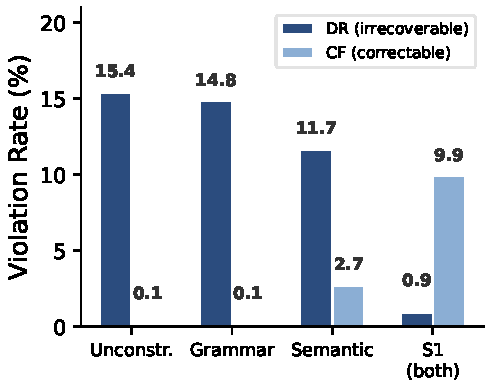
\includegraphics[width=\columnwidth]{figures/fig_violation_composition.pdf}
\caption{Violation composition across constraint configurations (SciERC, Qwen3-8B, zero-shot). As layers compose, DR (irrecoverable) drops 94\% while CF (correctable) becomes the sole residual, a severity downgrade from ontology-invalid to cross-triple type inconsistency.}
\label{fig:violation-composition}
\end{figure}

% Figures 4+5 side-by-side (spanning both columns)
\begin{figure*}[t]
\centering
\begin{minipage}[t]{0.48\textwidth}
  \centering
  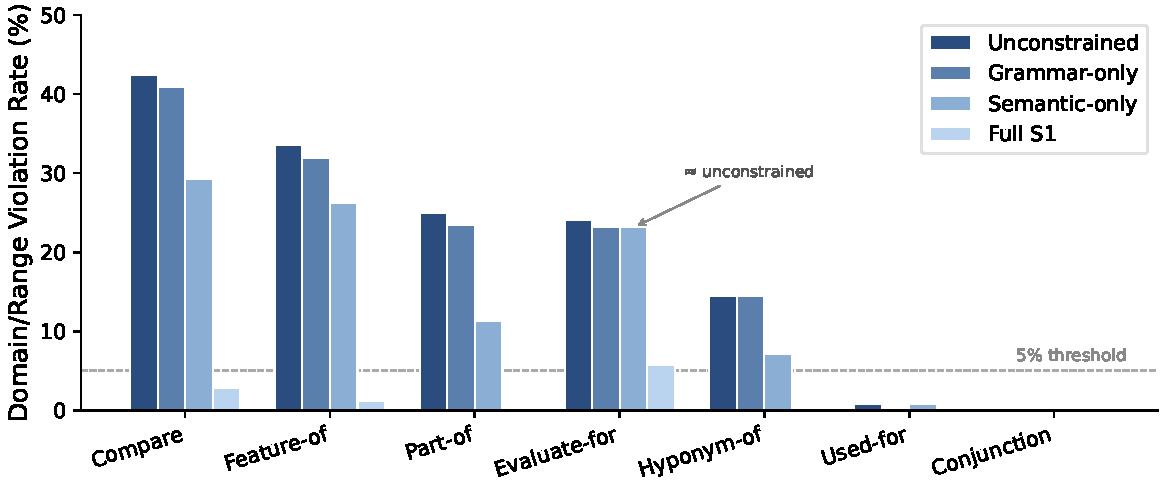
\includegraphics[width=\linewidth]{figures/fig2_per_relation_dr.pdf}
  \caption{Per-relation DR violation rates on SciERC (Qwen3-8B, unconstrained). Rates correlate with constraint tightness $\kappa(r)$. Llama-3.1-8B shows similar patterns (Appendix~\ref{app:llama-per-relation}).}
  \label{fig:per_relation_dr}
\end{minipage}%
\hfill
\begin{minipage}[t]{0.48\textwidth}
  \centering
  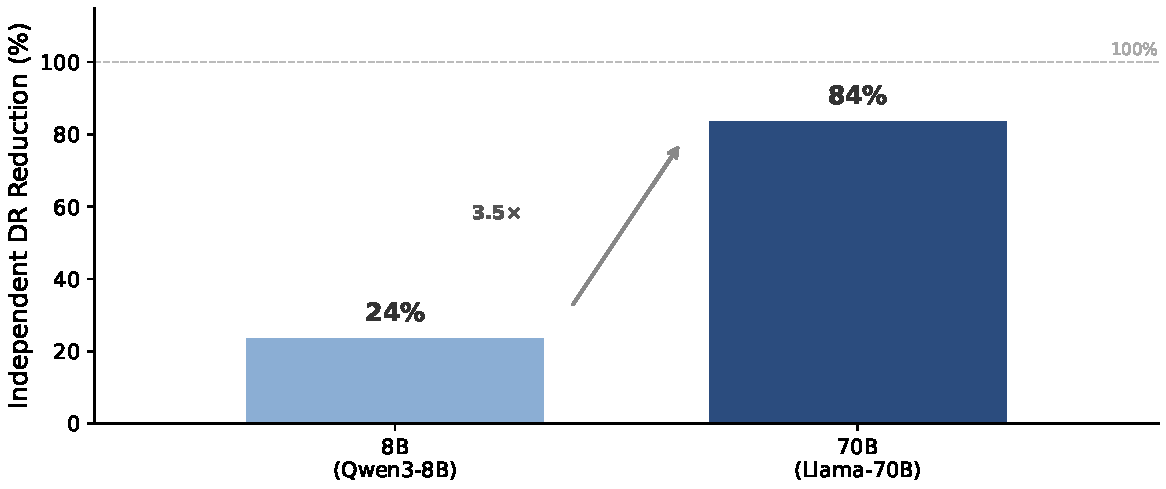
\includegraphics[width=\linewidth]{figures/fig_scale_dependency.pdf}
  \caption{Scale-dependent layer interaction: the semantic layer's independent DR reduction grows from 24\% at 8B to 84\% at 70B, reducing reliance on grammar-enforced vocabulary.}
  \label{fig:scale-dependency}
\end{minipage}
\end{figure*}


% Section 5 — SciERC Results (Draft)

\subsection{Ablation and Composability with Fine-Tuning}
\label{sec:scierc-results}

Table~\ref{tab:scierc-ablation} presents the five-way ablation on SciERC (Qwen3-8B, zero-shot, 551 documents); only the active constraint layers differ across rows.

% Figure 5 (scale-dependency) moved to figure* in section3_violation_landscape.tex

% Figure 6 (violation-composition) moved to section3_violation_landscape.tex for page 6 placement

% ──────────────────────────────────────────
%  Table: SciERC five-way ablation
% ──────────────────────────────────────────
\begin{table}[t]
\centering
\small
\setlength{\tabcolsep}{3.6pt}
\resizebox{\columnwidth}{!}{%
\begin{tabular}{@{}l rrrrrr rr@{}}
\toprule
& \multicolumn{6}{c}{\textbf{Violation Rates (\%)}}
& \multicolumn{2}{c}{\textbf{F1}} \\
\cmidrule(lr){2-7} \cmidrule(l){8-9}
\textbf{Mode}
  & DR\,$\downarrow$ & $\Delta$DR
  & RV\,$\downarrow$ & ET\,$\downarrow$ & CF & Tot.\,$\downarrow$
  & Rel.\,$\uparrow$ & Ent.\,$\uparrow$ \\
\midrule
Unconstrained
  & 15.37 & ---
  & 1.39  & 0.40
  & 0.08  & 15.45
  & 8.23  & 31.01 \\
Grammar
  & 14.84 & $\downarrow$3\%
  & \textbf{0} & \textbf{0}
  & 0.08  & 14.92
  & 8.23  & 30.98 \\
GCD-equiv.$^\dagger$
  & 15.26 & $\downarrow$1\%
  & \textbf{0} & \textbf{0}
  & 0.04  & 15.30
  & 8.75  & 30.91 \\
Semantic
  & 11.65 & $\downarrow$24\%
  & 1.51  & 0.40
  & 2.71  & 14.36
  & 8.15  & 31.01 \\
S1
  & \textbf{0.93} & $\downarrow$\textbf{94\%}
  & \textbf{0} & \textbf{0}
  & 9.90  & \textbf{10.83}
  & \textbf{8.36} & 30.98 \\
S2
  & 0.97  & $\downarrow$94\%
  & \textbf{0} & \textbf{0}
  & 8.03  & \textbf{9.00}
  & 8.03  & \textbf{31.90} \\
\bottomrule
\end{tabular}}%
\caption{Five-way ablation on SciERC (551 docs, Qwen3-8B, zero-shot).
$\Delta$DR: relative change vs.\ unconstrained; Tot.\ = DR + CF; bold = best (CF excluded).
F1 (\%). S1/S2 = single/two-pass (\S\ref{sec:strategies}).
Grammar = grammar-constrained decoding (GCD) ceiling~\cite{geng2023gcd}.
$\dagger$vLLM \texttt{guided\_json}~\cite{kwon2023vllm} (\S\ref{sec:constrained-baselines}).
Deterministic (greedy, $T{=}$0); robustness evidence in Table~\ref{tab:cross-model} and Appendices~\ref{app:bootstrap-effect-sizes},~\ref{app:prompt-sensitivity},~\ref{app:doc-length},~\ref{app:sampling}.}
\label{tab:scierc-ablation}
\end{table}

% ──────────────────────────────────────────
%  (a) Zero-shot diagnostic (compressed)
% ──────────────────────────────────────────
\paragraph{Zero-shot diagnostic.}
\emph{Does grammar-constrained decoding alone resolve DR violations?}
Table~\ref{tab:scierc-ablation} establishes that DR violations are pervasive (15--18\% across datasets) and that constraint layers interact non-additively: grammar-only achieves 3\% DR reduction on SciERC, semantic-only 24\%, but their composition yields 94\%, the \emph{empirical enabling dependency}.
On DocRED (96 relations, $\bar{\kappa}{=}0.842$), grammar-only \emph{increases} DR via \textit{latent violation surfacing}: forcing out-of-vocabulary (OOV)$\to$valid relation mapping exposes violations previously masked by vocabulary errors (Appendices~\ref{app:cross-model-zs},~\ref{app:docred-zs-ablation}).
Cross-model validation (3 models $\times$ 2 datasets; Table~\ref{tab:cross-model}) confirms DR drops of 76--99\% on SciERC and 42--90\% on DocRED, with R-F1 improving in 5/6 settings; post-hoc filtering achieves DR${=}$0\% but at 14--74\% rejection rates.
The DR-to-CF conversion is a severity downgrade, not an error introduction (Figure~\ref{fig:violation-composition}): DR violations produce ontology-invalid triples that corrupt downstream knowledge graphs and cannot be fixed without re-extraction, while CF (individually valid triples with cross-triple type inconsistency) can be resolved via fine-tuning, beam search, or post-hoc type-consistency reranking (TCR; eliminates all CF with bounded DR regression; Appendix~\ref{app:tcr}).
Zero-shot evaluation thus establishes violation prevalence and constraint interaction; fine-tuning demonstrates practical elimination.

% Figure 6 (violation-composition) moved earlier in source for page 6 placement

% Cross-model table is in §6.1 (Table~\ref{tab:cross-model}).

% ──────────────────────────────────────────
%  (e) Composability with Fine-Tuning (expanded)
% ──────────────────────────────────────────
\paragraph{Composability with fine-tuning.}
\label{sec:composability}
\emph{Does OntoCoDec retain value after fine-tuning?}
Fine-tuning alone reduces DR to 0.5--2\% but leaves residual violations on tight-constraint relations (Table~\ref{tab:composability}; full fine-tuning in Appendix~\ref{app:full-ft}); adding S1 yields DR\,$\leq$\,0.21\% with no significant $\Delta$R-F1 (Bonferroni-corrected; 95\% CIs $\subseteq [-0.69, {+}0.25]$\,pp; removed triples are 97.6--100\% false positives; Appendix~\ref{app:downstream-impact}).
Under fine-tuning, grammar becomes a no-op ($\Delta$DR$<$0.2\,pp), making the semantic layer the sole DR defense (41--69\% on SciERC, 2--75\% on DocRED; Appendix~\ref{app:ft-ablation}); three relations with $\kappa \geq 0.36$ retain DR, all eliminated by S1 (Appendix~\ref{app:lora-per-relation}).
CF drops from $+$9.82\,pp (zero-shot) to $+$1.18\,pp (fine-tuned), concentrated in \textsc{Generic}$\leftrightarrow$X ambiguity (63.3\%; Appendices~\ref{app:cf-distribution},~\ref{app:cascade-analysis}); beam ($k{=}4$) achieves near-zero violations at 8B (R-F1 43--46; \S\ref{sec:beam-results}).

% CF analysis folded into composability paragraph above; details in Appendices~\ref{app:cf-distribution},~\ref{app:cascade-analysis}.
% Table 2 (composability) moved to section5_crossmodel_draft.tex for page 8 placement

% ──────────────────────────────────────────
%  (f) Downstream impact of DR elimination
% ──────────────────────────────────────────
\paragraph{Downstream impact.}
\label{sec:downstream-impact}
Constraint removal affects only 0.24\% of gold triples; error analysis confirms only 0.2\% of false negatives were blocked by constraints (Appendices~\ref{app:lucky-violations},~\ref{app:error-analysis},~\ref{app:case-studies}).
The 36 residual DR violations across fine-tuned settings decompose into entity type errors (39\%), schema gaps (33\%), and relation/direction errors (28\%); the irreducible floor is $\sim$3 violations (Appendix~\ref{app:residual-dr-analysis}).

% Section 5 — Cross-Model Validation (compressed)

\subsection{Cross-Model Validation}
\label{sec:cross-model}

% Figure 7 (heatmap) definition moved to section5_runtime.tex for right-column placement on p8.

S1 eliminates RV and ET for all models ($\leq$0.03\%); DR drops 76--99\% on SciERC and 42--90\% on DocRED (Figure~\ref{fig:crossmodel-heatmap}; Table~\ref{tab:cross-model}), with R-F1 improving in 5/6 settings.
Post-hoc filtering achieves DR${=}$0\% but at 14--74\% rejection rates (Appendix~\ref{app:posthoc-extended}).

% Table 2 (composability) moved to section5_runtime.tex for page 8 placement

% Section 5 — Event Extraction on WikiEvents (summary; full results in Appendix)

\subsection{Event Extraction Validation}
\label{sec:wikievents}

\emph{Does OntoCoDec generalize beyond relation extraction?}
Zero-shot evaluation on WikiEvents (246 documents, 3 models; Appendices~\ref{app:wikievents-pilot},~\ref{app:wikievents},~\ref{app:wikievents-kappa}) confirms constraint applicability to event extraction, with event-vocabulary (EV) and role-vocabulary (RoV) violations eliminated across all models; fine-tuning composability is preliminary ($n{=}20$).

% Runtime overhead (inline paragraph, no subsection header to save space)

\paragraph{Runtime overhead.}
\label{sec:runtime}
\emph{What is the practical overhead?}
S1 overhead is $+$13.1\% on SciERC, lower on DocRED due to amortization over longer sequences; under LoRA, $+$10.0\% with 37\% lower absolute latency (Appendix~\ref{app:ft-latency}).
Constraint compilation is one-time $<$0.5\,s; scaling benchmarks confirm constant overhead (2--3\%) up to 200 entity types and 1{,}000 relations (Appendix~\ref{app:scalability}).

\paragraph{Beam search compatibility.}
\label{sec:beam-results}
\emph{Can beam search mitigate CF violations?}
With LoRA, beam search~\cite{anderson2017guided} achieves near-zero violations at 8B on both SciERC and DocRED (DR${=}$RV${=}$ET${=}$0\% for Llama-3.1-8B; $\leq$0.01\% residual CF for Qwen3-8B); at 70B, beam $k{=}4$ achieves DR${=}$RV${=}$ET${=}$0\% with one residual CF on SciERC (Appendix~\ref{app:beam-search}).
A beam-width sweep ($k \in \{1,2,4,8\}$) reveals $k{=}2$ as Pareto-optimal: R-F1 44.60, CF 0.11\%, at 1.18$\times$ greedy S1 latency; $k{=}4$ achieves CF${=}$0\% at 1.39$\times$ (Figure~\ref{fig:beam-pareto}; Appendix~\ref{app:beam-search}).
This yields three deployment tiers: greedy S1 ($+$10\%, DR${\leq}$0.21\%, CF${\leq}$1.4\%), beam $k{=}2$ (1.18$\times$, near-zero CF), and beam $k{=}4$ (1.39$\times$, near-zero violations at 8B).

% ──────────────────────────────────────────
%  Table: Fine-tuning composability (moved here for page 8 placement)
% ──────────────────────────────────────────
\begin{table}[t]
\centering
\small
\setlength{\tabcolsep}{3pt}
\resizebox{\columnwidth}{!}{%
\begin{tabular}{@{}lll rrrr r@{}}
\toprule
\textbf{Model} & \textbf{Dataset} & \textbf{Mode}
  & \textbf{DR\,$\downarrow$} & \textbf{CF}
  & \textbf{R-F1\,$\uparrow$} & \textbf{E-F1\,$\uparrow$}
  & \textbf{$\Delta$DR} \\
\midrule
\multirow{4}{*}{Qwen3-8B}
  & \multirow{2}{*}{SciERC}
    & Unconstr.\ &  1.95 & 0    & 43.86 & 67.05 & --- \\
  & & S1    & \textbf{0} & 1.18 & 43.77 & 67.05 & $\downarrow$100\% \\
\cmidrule(l){2-8}
  & \multirow{2}{*}{DocRED}
    & Unconstr.\ &  0.76 & 0.12 & 40.86 & 82.15 & --- \\
  & & S1    & 0.01 & 0.41 & 40.56 & 81.43 & $\downarrow$98.7\% \\
\midrule
\multirow{4}{*}{\shortstack[l]{Llama\\3.1-8B}}
  & \multirow{2}{*}{SciERC}
    & Unconstr.\ &  1.11 & 0    & 45.45 & 67.76 & --- \\
  & & S1    &  0.09 & 0.46 & 45.47 & 67.76 & $\downarrow$92\% \\
\cmidrule(l){2-8}
  & \multirow{2}{*}{DocRED}
    & Unconstr.\ &  0.49 & 0.08 & 43.72 & 83.93 & --- \\
  & & S1    &  0.21 & 0.21 & 43.78 & 83.94 & $\downarrow$57\% \\
\bottomrule
\end{tabular}}%
\caption{Fine-tuning composability: LoRA $\times$ unconstrained vs.\ S1 on SciERC (551 docs) and DocRED (998 dev docs).
F1 (\%). No $\Delta$R-F1 is significant (Bonferroni-corrected; details in text); all DR reductions are ($p{<}0.001$; power analysis in Appendix~\ref{app:power-analysis-full}).
E-F1 (entity F1) includes parse-failure documents (Qwen PF (parse failure): 7--8\%; Llama PF: 2--3\%).}
\label{tab:composability}
\end{table}

\paragraph{70B-class validation.}
\label{sec:70b-results}
\emph{Does the layer interaction change with model scale?}
On Llama-3.1-70B (AWQ INT4), zero-shot S1 eliminates DR on both datasets (SciERC 6.41\%\,$\to$\,0\%, DocRED 14.98\%\,$\to$\,0\%); semantic-only achieves 84\% DR reduction vs.\ 8B's 24\% (Figure~\ref{fig:scale-dependency}).
LoRA confirms composability: DR\,$\to$\,0\% on both datasets (R-F1 44--45; Appendices~\ref{app:70b-ablation},~\ref{app:70b-docred-zs},~\ref{app:70b-docred},~\ref{app:quantization}).

\paragraph{GCD comparison.}
\label{sec:constrained-baselines}
Our grammar-only row (Table~\ref{tab:scierc-ablation}) is analytically equivalent to GCD~\cite{geng2023gcd}/BoostCD~\cite{boostcd2025}; vLLM \texttt{guided\_json}~\cite{kwon2023vllm} confirms this (DR${=}$15.26\%; Appendix~\ref{app:gcd-comparison}).
The ${\sim}$15\% residual DR is the gap our semantic layer addresses (94\% total reduction).


% === §7 Discussion and Conclusion ===
\section{Discussion and Conclusion}
\label{sec:discussion}
% Section 7 — Discussion and Conclusion

% ──────────────────────────────────────────
%  Figure: Cross-Model Heatmap (placed here for right-column [t] on p8)
% ──────────────────────────────────────────
\begin{figure}[t]
\centering
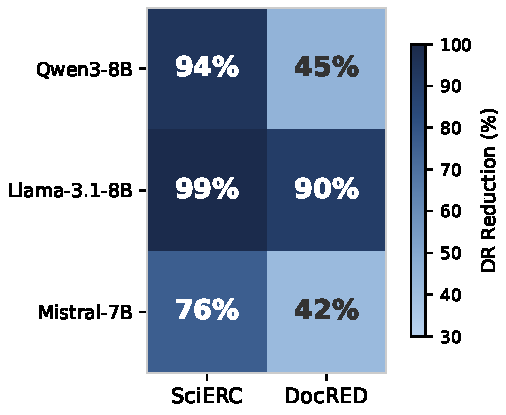
\includegraphics[width=0.75\columnwidth]{figures/fig_crossmodel_heatmap.pdf}
\caption{DR reduction (\%) across 3 models $\times$ 2 datasets (zero-shot S1). Calibrated models (Qwen, Llama) achieve $\geq$90\% on SciERC; DocRED's higher $\bar{\kappa}$ reduces effectiveness. Full violation breakdown in Table~\ref{tab:cross-model} (Appendix~\ref{app:cross-model-zs}).}
\label{fig:crossmodel-heatmap}
\end{figure}

Neither layer alone suffices: grammar-only achieves 3\% DR reduction, semantic-only 24\%, but their composition yields 94\%, an enabling dependency that weakens at scale (84\% at 70B).
This non-additive interaction arises because the grammar layer provides a structured prerequisite: by restricting relation tokens to $\mathcal{R}$ and entity type tokens to $\mathcal{E}$, it ensures the semantic layer receives well-formed inputs on which domain/range lookups can operate.
Without grammar-enforced vocabulary membership, the semantic layer cannot reliably identify which relation governs a given type position.

OntoCoDec composes both layers, reducing DR to $\leq$\,0.21\% across model families and datasets ($\pm$0.3\,pp R-F1).
The residual DR$\to$CF conversion is a severity downgrade rather than an error introduction: DR violations produce ontology-invalid triples that corrupt downstream knowledge graphs and require re-extraction, while CF violations (cross-triple type inconsistency) preserve individually valid triples and are resolvable via beam search or post-hoc reranking.
Beam $k{=}4$ achieves near-zero violations at 8B, making generative IE reliably schema-compliant.


% === Limitations ===
\section*{Limitations}

Per-triple enforcement creates a DR$\leftrightarrow$CF trade-off; global type consensus during decoding remains future work.
Evaluation covers 8B/70B models on two RE and one EE dataset; smaller-model and non-English generalization is untested.
Empirical type constraints are derived from training data (99\%+ coverage) rather than formal ontology specifications; rare type combinations absent from training data fall back to grammar-only enforcement.

% === Bibliography ===
\bibliography{relwork_new_entries}

% === Appendix ===
\appendix

% Appendix — Prompt Templates

\section{Prompt Templates}
\label{app:prompts}

All experiments use the same prompts across constrained and unconstrained decoding; constraints are applied at the logit level, not through prompt modification.
Table~\ref{tab:prompts} shows the system and user prompts for each dataset.

\begin{table*}[t]
\centering
\small
\begin{tabular}{@{}p{0.95\textwidth}@{}}
\toprule
\textbf{SciERC --- System Prompt (Unconstrained \& Constrained)} \\
\midrule
\texttt{You are an expert information extraction system for scientific texts. Extract entities and relations from the given text.} \\[4pt]
\texttt{Entity types: Task, Method, Material, Metric, OtherScientificTerm, Generic} \\
\texttt{Relation types: Used-for, Feature-of, Hyponym-of, Part-of, Compare, Conjunction, Evaluate-for} \\[4pt]
\texttt{Output a JSON object with:} \\
\texttt{- "entities": list of \{"text": "...", "type": "..."\}} \\
\texttt{- "relations": list of \{"head": "...", "tail": "...", "type": "...", "head\_type": "...", "tail\_type": "..."\}} \\[4pt]
\texttt{Output ONLY valid JSON, no explanation.} \\
\midrule
\textbf{SciERC --- User Prompt} \\
\midrule
\texttt{Extract all entities and relations from this scientific text:} \\
\texttt{"\{text\}"} \\
\texttt{Output JSON:} \\
\midrule
\midrule
\textbf{DocRED --- System Prompt (Unconstrained \& Constrained)} \\
\midrule
\texttt{You are an information extraction system. Extract all entities and relations from the following document.} \\[4pt]
\texttt{Entity types: PER, ORG, LOC, TIME, NUM, MISC} \\[4pt]
\texttt{Relation types: country, instance of, performer, ...\ (96 Wikidata relation types; full list omitted for space)} \\[4pt]
\texttt{Output a JSON object with exactly this structure:} \\
\texttt{\{"entities": [\{"text": "entity name", "type": "ENTITY\_TYPE"\}],} \\
\texttt{\ "relations": [\{"head": "head entity", "tail": "tail entity", "type": "relation name",} \\
\texttt{\ \ "head\_type": "ENTITY\_TYPE", "tail\_type": "ENTITY\_TYPE"\}]\}} \\[4pt]
\texttt{Output ONLY the JSON, no other text.} \\
\midrule
\textbf{DocRED --- User Prompt} \\
\midrule
\texttt{(Document text provided inline in the user message.)} \\
\bottomrule
\end{tabular}
\caption{Extraction prompts used in all experiments.
The same prompts are used for both unconstrained and constrained decoding; OntoCoDec's constraints operate at the logit level during generation.
Schema-informed prompts (\S\ref{sec:violation_landscape}) additionally include valid (head type, tail type) pairs per relation.}
\label{tab:prompts}
\end{table*}

\section{Extended Related Work}
\label{app:related_work}

% ===========================================================================
% Paradigm 1: Grammar-Constrained Decoding
% ===========================================================================
\paragraph{Grammar-Constrained Decoding.}
Recent work has established efficient algorithms for restricting LLM outputs to conform to context-free grammars, making grammar-constrained decoding the de facto standard for obtaining structured output from language models.
XGrammar~\cite{dong2025xgrammar} partitions the vocabulary into context-independent and context-dependent tokens and maintains persistent pushdown automata across decoding steps, achieving up to 100$\times$ speedup over prior CFG-constrained decoding methods.
Outlines~\cite{willard2023outlines} reformulates constrained generation as finite-state machine transitions with offline vocabulary indexing, which enables efficient enforcement of regular-expression and JSON-schema constraints without runtime overhead per token.
LMQL~\cite{beurer-kellner2023lmql} introduces a declarative query language that compiles type, length, and regex constraints into token-level masks, providing a programmable interface for specifying multi-variable output structures.
These systems ensure that every generated token belongs to a grammar-valid continuation, but they do not address the \emph{distribution distortion} introduced by naive token masking.
A parallel line of work tackles this problem directly: DOMINO~\cite{beurer-kellner2024domino} minimizes distributional divergence during CFG enforcement by formulating mask selection as an optimization problem, and ASAp~\cite{park2024grammar} provides a provably unbiased sampling algorithm that preserves the original LM distribution under grammar constraints.
Together, these advances have made grammar-constrained decoding both fast and statistically principled, and provide a robust foundation for structured generation.
However, all of these methods operate exclusively at the syntactic level: they ensure format validity (e.g., well-formed JSON, valid enum values) but cannot enforce cross-field semantic constraints such as ontology domain/range rules that depend on previously generated content.
This syntactic-only limitation motivates OntoCoDec's semantic extension: our grammar layer builds on XGrammar for structural (JSON schema and enum) constraints, while a second semantic layer enforces relational type constraints that are inherently beyond the expressive power of context-free grammars.

% ===========================================================================
% Paradigm 1.5: Semantic Constrained Decoding for Code
% ===========================================================================
\paragraph{Semantic Constrained Decoding for Code.}
In programming-language generation, constrained decoding has been extended beyond syntax to enforce semantic properties such as type correctness; this work demonstrates that richer-than-CFG constraints can be compiled into token-level filtering.
In the text-to-SQL domain, PICARD~\cite{scholak2021picard} maintains an incremental SQL parsing state that rejects tokens violating syntax or referencing non-existent database columns at each decoding step, achieving state-of-the-art results on Spider and CoSQL without modifying model weights.
While mechanistically similar to OntoCoDec's token-level filtering, PICARD operates over a \emph{fixed, fully enumerated} schema (database table and column names known before decoding begins).
In contrast, OntoCoDec's entity registry is populated \emph{during} generation as entity spans are extracted from free text; constraint sets evolve with the decoding prefix, a fundamental distinction between querying a known schema and extracting from unstructured text.
Synchromesh~\cite{synchromesh_iclr2022} pioneers Constrained Semantic Decoding (CSD), which enforces syntax, type, and scope constraints simultaneously during code generation from pre-trained LMs without fine-tuning; this establishes that semantic constraints can be expressed as dynamic token masks conditioned on the generation prefix.
MGD~\cite{mgd_neurips2023} uses static-analysis monitors to perform incremental type checking at decode time; SantaCoder-1.1B with MGD outperforms text-davinci-003 on repository-level code completion by ensuring that every generated identifier is type-correct with respect to the surrounding code context.
Most recently, \citet{pldi2025_type_constrained_codegen} compile full type systems, including generic types and subtyping, into prefix automata for token-level logits masking and reduce compilation errors by over 50\%.
This last system is the closest mechanistic analog to OntoCoDec, applying the same ``type system $\to$ automaton $\to$ logits mask'' pipeline, though in a fundamentally different domain.
The key technical difference lies in the constraint structure: programming-language type systems feature deep subtyping hierarchies and parametric polymorphism, whereas IE ontology axioms specify flat domain/range sets; a relation $R$ accepts head entities from set $\mathcal{D}(R)$ and tail entities from set $\mathcal{R}(R)$, with no subtype chains.
Conversely, IE introduces a challenge absent in code generation: the constraint target (entity type) must be inferred from free-text spans rather than read from declared type annotations, so a stateful entity registry must track extracted types during autoregressive generation.
These methods collectively demonstrate that semantic (type) constraints at decode time are both feasible and highly effective, but exclusively in the code domain where type systems are formally specified.
OntoCoDec is the first to \emph{automatically compile} IE ontology axioms, including domain/range constraints, into token-level decoding masks for information extraction, migrating the type-constrained decoding paradigm from code generation to IE.

% ===========================================================================
% Paradigm 2: Vocabulary/Type-Constrained Generation
% ===========================================================================
\paragraph{Vocabulary and Type-Constrained Generation.}
The idea of enforcing entity-type compatibility constraints for information extraction dates back to pre-neural methods.
\citet{roth_yih_2004} formulate joint entity and relation identification as an integer linear program (ILP) that enforces type constraints (e.g., \textsc{Emp-Org} only between \textsc{Per} and \textsc{Org} entities); this establishes the foundational principle that relational type compatibility should be a hard constraint, not a soft preference learned from data.
In the autoregressive era, GENRE~\cite{decao2021genre} pioneers trie-based constrained beam search for autoregressive entity retrieval, restricting each decoding step to tokens consistent with valid entity names from a predefined catalog.
GenIE~\cite{josifoski2022genie} extends this approach to end-to-end information extraction with state-based constraints that enforce valid triple structures, achieving strong performance on closed-world knowledge base population, though it requires task-specific fine-tuning on the target schema.
AdaKGC~\cite{adakgc_emnlp2023} introduces schema-constrained dynamic decoding with trie-based prefix trees that adapt to the target schema, enforcing that generated entity and relation names belong to a predefined inventory, a vocabulary-level constraint that ensures name validity but does not verify type compatibility between a relation and its arguments.
GCD~\cite{geng2023gcd} provides a unified grammar-constrained decoding framework for structured NLP tasks including IE, introducing input-dependent grammars that adapt constraints based on the source text. GCD is the closest precursor to OntoCoDec in applying logits masking to IE, though limited to syntactic constraints.
NeuroLogic Decoding~\cite{lu2021neurologic} expresses lexical inclusion and exclusion constraints as predicate logic formulas enforced during beam search, offering a general mechanism for token-level control that can encode vocabulary membership but not relational type rules.
These approaches constrain \emph{which tokens} can appear (vocabulary membership) but not \emph{which type combinations} are valid for a given relation.
OntoCoDec's semantic layer enforces relational constraints (e.g., that the head entity of relation $R$ must belong to type set $\mathcal{D}(R)$) which cannot be expressed as static vocabulary restrictions because the valid set depends on the relation type generated earlier in the same sequence.
While Roth \& Yih's ILP formulation shares the same type-compatibility motivation, it operates as a post-hoc reranker over discrete candidates; OntoCoDec integrates enforcement directly into autoregressive decoding, preventing violations rather than filtering them.

% ===========================================================================
% Paradigm 3: Structural Constraints for IE
% ===========================================================================
\paragraph{Structural Constraints via Training and Prompting.}
An orthogonal approach encodes IE output structure through model training or prompt design rather than decoding-time enforcement, relying on learned representations to produce schema-compliant outputs.
UIE~\cite{lu2022uie} defines a Structured Extraction Language and trains a unified text-to-structure model across 13 IE datasets, relying on large-scale pre-training to internalize output format constraints.
GoLLIE~\cite{sainz2024gollie} expresses annotation guidelines as Python dataclass definitions and fine-tunes Code-LLaMA to generate typed code, achieving strong zero-shot transfer to unseen IE schemas through the implicit type structure of programming languages.
KnowCoder~\cite{knowcoder_acl2024} takes this further by encoding 29K entity types from Wikidata as a Python class hierarchy, training a Code-LLM to generate structured extraction code that implicitly respects type inheritance, the most comprehensive schema-as-code approach to date.
CodeIE~\cite{li2023codeie} similarly reformulates IE as code generation, using the structural regularity of programming languages to reduce output format errors.
ADELIE~\cite{qi2024adelie} uses supervised fine-tuning (SFT) and Direct Preference Optimization (DPO) to align LLMs on IE tasks, achieving state-of-the-art results among open-source models while preserving general capabilities, though compliance with ontological constraints remains a learned soft preference rather than a hard constraint.
In the supervised setting, joint entity-relation architectures such as SpERT~\cite{eberts2020spert} and PFN~\cite{yan2021pfn} enforce type consistency implicitly through shared representations: SpERT classifies entity spans and relation pairs in a single BERT pass with span-level negative sampling, while PFN decomposes feature encoding into entity-specific, relation-specific, and shared partitions via gating mechanisms.
These models achieve strong performance but are limited to fixed, predefined schemas and cannot generalize to unseen ontologies without retraining, precisely the ontology-portable scenario requiring no constraint-specific training that OntoCoDec targets.
EnriCo~\cite{zaratiana2024enrico} applies Answer Set Programming (ASP) constraints during decoding of joint entity-relation extraction models, enforcing structural type compatibility at generation time. This is a decoding-time approach, though with model-specific, manually authored constraints rather than ontology-driven compilation.
Training-based methods provide \emph{soft} structural guidance: the model learns to prefer valid outputs but cannot enforce compliance at inference time, as demonstrated by non-trivial violation rates even in fine-tuned systems.
Importantly, training-based and decoding-time approaches are complementary rather than competing: a system like GoLLIE could be combined with OntoCoDec's constraint layers, using fine-tuning to maximize the probability of valid outputs while decoding-time enforcement eliminates residual violations.
OntoCoDec provides \emph{hard} decoding-time enforcement that requires no constraint-specific training, is automatically compiled from IE ontologies, and composable with any of these training-based approaches.

% ===========================================================================
% Paradigm 4: Type-Checking / Ontology Validation
% ===========================================================================
\paragraph{Post-hoc Ontology Validation.}
Rather than constraining generation, several methods validate LLM outputs against ontological rules after generation, applying a detect-then-fix paradigm.
ODKE+~\cite{khorshidi2025odke} dynamically generates ontology snippets containing domain/range constraints as prompt context, achieving 98.8\% precision across 195 predicates at web scale, but constraint adherence relies on prompt-level guidance, not enforcement, leaving residual violations unaddressed.
SPIRES/OntoGPT~\cite{spires_2024} provides an ontology-based extraction framework that grounds LLM outputs against OBO ontologies post-generation: it validates extracted entities and relations through ontology lookup and corrects mismatches in a second pass, the prompt-then-validate paradigm in the biomedical domain.
OntoLogX~\cite{ontologx_2025} applies Shapes Constraint Language (SHACL) validation to LLM-generated knowledge graphs, iteratively re-prompting the LLM to correct constraint violations and reducing them by approximately 10$\times$ across multiple correction rounds. This demonstrates the detect-then-fix paradigm's effectiveness but also its inherent multi-pass cost.
\citet{upadhyay2023openie} inject entity-type knowledge as constraints into Open IE via both constrained inference and constraint-aware training, improving F1 by 29\% on CaRB, though their constrained inference operates over a discrete candidate set rather than during autoregressive generation.
\citet{regino2025kgcurator} propose a multi-stage LLM pipeline for validating Resource Description Framework (RDF) triple insertions against RDF Schema (RDFS) domain/range constraints, where each validation step requires a separate LLM call, effective but computationally expensive at scale.
RELATE~\cite{olasunkanmi2025relate} addresses the alignment gap between LLM-extracted biomedical relations and standardized ontology predicates through a three-stage pipeline: ontology preprocessing with predicate embeddings, similarity-based retrieval via SapBERT, and LLM-based reranking with negation handling, achieving 94\% accuracy@10 on ChemProt.
While RELATE demonstrates effective ontology grounding for relation extraction, its constraints are applied \emph{post-extraction} through retrieval and reranking rather than during generation, and it requires domain-specific embedding models trained on biomedical corpora.
OntoCoDec enforces ontology constraints \emph{during} autoregressive decoding and requires no additional trained components beyond the base LLM.
Concurrently, \citet{zhou2026ontologytools} compile Web Ontology Language (OWL) ontologies into executable tool interfaces within The World Avatar framework; LLM agents must invoke ontology-aware tools that enforce semantic constraints during knowledge graph construction from scientific text.
This ``ontology-to-tools'' approach shares OntoCoDec's philosophy of compiling formal ontological knowledge into runtime enforcement mechanisms, but operates at the tool-call level (constraining which API functions the agent invokes) rather than at the token level (constraining which tokens the decoder produces), and requires an agentic multi-step workflow rather than single-pass autoregressive generation.
\citet{ekaw2024_ontology_beam} introduce ontology-constrained beam scoring for clinical summarization, applying soft biases (not hard masks) during beam search to steer outputs toward ontology-compliant terms, a middle ground between unconstrained generation and hard enforcement that reduces but cannot eliminate violations.
Post-hoc validation detects violations after generation and requires rejection or correction cycles that waste compute. In our setting, 15.37\% of generated triples contain domain/range violations under unconstrained decoding, a substantial waste of generation effort.
OntoCoDec \emph{prevents} violations during decoding, redirecting probability mass to valid alternatives rather than discarding invalid outputs, with only marginal overhead from logits masking compared to the cost of regenerating or correcting violated triples.
Soft-constraint approaches such as ontology-weighted beam scoring reduce violation frequency but cannot eliminate it, whereas OntoCoDec substantially reduces violations (DR$\downarrow$94\% on SciERC, $\downarrow$45--90\% on DocRED depending on model).

% ===========================================================================
% Paradigm 5: Constrained Decoding Quality Concerns
% ===========================================================================
\paragraph{Quality Impact of Constrained Decoding.}
A growing body of work raises concerns that constrained decoding degrades LLM generation quality, particularly for reasoning-intensive tasks where format enforcement interferes with chain-of-thought processes.
\citet{tam2024letmespeak} conduct a comprehensive evaluation showing that rigid format constraints (JSON, XML) harm performance on math and multi-hop QA benchmarks but \emph{benefit} classification-style tasks such as slot filling, a distinction directly relevant to IE, which is fundamentally an extraction (classification-like) task rather than a reasoning task.
CRANE~\cite{banerjee2025crane} provides theoretical analysis of why restricting outputs to narrow grammars suppresses chain-of-thought reasoning by eliminating intermediate reasoning tokens, and proposes an alternating strategy between unconstrained reasoning phases and constrained output phases to mitigate this effect.
\citet{schall2025hiddencost} conduct a systematic study across 11 models and multiple benchmarks, finding 10--30\% semantic correctness degradation on reasoning tasks under structural constraints, with larger models showing greater absolute degradation.
\citet{zhou2026snowballing} identify ``structure snowballing,'' a failure mode where format compliance cognitive load traps models in repetitive structural patterns rather than improving reasoning during self-correction iterations.
These findings establish a legitimate concern for constrained decoding in reasoning-heavy applications.
However, information extraction occupies a fundamentally different regime: the model extracts entities and relations from input text rather than generating novel reasoning chains, and \citet{tam2024letmespeak}'s own results show that extraction-style tasks are robust to, or even benefit from, format constraints.
OntoCoDec addresses this concern empirically: domain/range violations decrease by 94\% on SciERC (15.37\%$\to$0.93\%) and 45--90\% on DocRED across two models, with F1-neutral impact on SciERC ($+$0.13pp, $p{=}0.58$) and significant R-F1 gains on DocRED (Qwen $p{<}0.001$, Llama $p{=}0.013$).
Critically, OntoCoDec's constraints target only type tokens (entity types, relation labels), leaving free-text spans (entity surface forms and their boundaries) entirely unconstrained, which minimizes the distribution distortion that causes quality degradation in reasoning tasks.
A two-pass variant (S2), explored in ablation (Section~5), separates extraction and constraint enforcement into distinct passes, analogous to CRANE's alternating strategy; however, our primary single-pass approach already avoids reasoning interference by constraining only type tokens while leaving free-text spans unconstrained.

% ===========================================================================
% Our Approach
% ===========================================================================
\paragraph{Our Approach.}
OntoCoDec occupies a unique position in this landscape: it is the first system to \emph{automatically compile} IE ontologies, including domain/range axioms, into token-level semantic masks, extending grammar-constrained decoding from syntactic to semantic enforcement without manually authored rules.
Unlike vocabulary-constrained methods that restrict individual tokens to a fixed set, OntoCoDec enforces \emph{cross-field relational constraints} through a stateful entity registry that tracks extracted types during autoregressive generation; constraint evaluation is dynamic and depends on previously decoded content.
This approach is orthogonal to supervised IE methods and applicable to autoregressive LMs with logits access without model modification or additional training (evaluated on 7B--70B models across three tokenizer families).
Unlike training-based IE systems, OntoCoDec requires no constraint-specific training and substantially reduces type violations at inference time (DR$\downarrow$94\% on SciERC, $\downarrow$45--90\% on DocRED); unlike post-hoc validation, it prevents violations rather than detecting them, redirecting probability mass to valid alternatives with significant R-F1 gains on DocRED ($p \leq 0.013$) and F1-neutral impact on SciERC.
The two constraint layers, grammar (structural) and semantic (relational), compose via bitwise AND with a scale-dependent interaction: the grammar layer ensures every generated type token belongs to the valid vocabulary, which enables the semantic layer to look up and enforce domain/range rules for that type.

% Appendix B — Extended Discussion
% Contains discussion paragraphs moved from the main text during compression.

\section{Extended Discussion}\label{app:discussion}

%%% CF Dual Mechanism %%%

\paragraph{CF Dual Mechanism.}
CF violations arise from two distinct mechanisms:
(1)~\emph{Registry override}: the semantic constraint forces a domain-compatible type that conflicts with the entity's previously registered type.
The entity appears in multiple relations with different type requirements, and the per-relation mask selects the locally valid type without consulting prior assignments.
(2)~\emph{Grammar-first fallback} (\S\ref{sec:interaction}): when the semantic mask conflicts with all grammar-valid tokens, the semantic layer is dropped entirely, allowing the grammar layer to generate any structurally valid type, which may differ from the entity's registered type.

These mechanisms have sharply different model profiles.
Qwen3-8B triggers zero grammar-first fallbacks across all experiments, attributing 100\% of its CF violations to registry override.
Llama-3.1-8B, by contrast, triggers 5{,}882 fallbacks on SciERC (10.7 per document) and 57{,}825 on DocRED (63.8 per document), making grammar-first fallback the dominant CF source.
This asymmetry is consistent with the cross-model CF gap: Qwen achieves CF\,=\,2.57\% on DocRED vs.\ Llama's 12.02\%, despite both using identical constraint configurations.
The difference traces to Llama's less calibrated type predictions, which more frequently conflict with the semantic mask's valid set, triggering fallback.

%%% Fallback Behavior and Effective Coverage %%%

\paragraph{Fallback Behavior and Effective Coverage.}
\label{app:fallback-coverage}
The two-layer architecture produces two distinct fallback mechanisms with different semantic consequences.
\emph{Grammar-first fallback} occurs when $S(t) \cap G(t) = \emptyset$: the semantic layer deactivates as a safety valve, preserving structural validity at the cost of potential type violations.
The token-level fallback rate (36.6\% on SciERC Llama) is inflated by continuation tokens of multi-token type names (e.g., \textsc{OtherScientificTerm}, averaging 2.87 BPE tokens); at semantically meaningful first-token positions, the rate is 0.04--5.7\% (zero-shot) and drops to $\leq$\,0.11\% under fine-tuning.
These events account for the residual DR that persists after constraint enforcement.
\emph{Registry-consistent fallback} (4.5\%) occurs when the entity's registered type conflicts with domain/range constraints; the system defaults to the registered type for cross-triple consistency.
Together, these mechanisms produce the characteristic profile of composable constraint systems: residual DR traces to grammar-first fallback events, while CF violations arise from registry override events where per-relation enforcement assigns conflicting types.

We define \emph{effective semantic constraint coverage} as $1 - f_{\text{gf}}$, where $f_{\text{gf}}$ is the grammar-first fallback rate.
On SciERC, Llama-3.1-8B shows $f_{\text{gf}} = 36.6\%$ (6{,}237 of 17{,}024 mask calls), yielding 63.4\% effective coverage.
On DocRED, by contrast, Qwen3-8B shows $f_{\text{gf}} = 0.08\%$ (46 of 54{,}859), yielding 99.9\% coverage.
The large discrepancy is primarily a tokenization artifact: SciERC entity types are multi-token (e.g., \textsc{OtherScientificTerm}, averaging 2.87 mask calls per type field), and continuation tokens necessarily conflict with the semantic mask, inflating the per-mask-call fallback rate.
DocRED types (\textsc{PER}, \textsc{ORG}, \textsc{LOC}, \textsc{TIME}, \textsc{NUM}, \textsc{MISC}) are all single-token, eliminating this inflation.
This metric directly quantifies the layer interaction (\S\ref{sec:interaction}): it measures the fraction of decoding steps where both constraint layers are jointly active, providing a fine-grained view beyond aggregate violation rates.
Qwen3-8B, with zero grammar-first fallbacks, achieves 100\% effective coverage on SciERC, consistent with its lower residual DR (0.93\% vs.\ Llama's 0.08\%).

%%% Fallback Causal Tracing %%%

\paragraph{Fallback Causal Tracing.}
\label{app:causal-tracing}

To establish that grammar-first fallback is the \emph{sole} mechanism producing residual DR violations, we instrument the constraint processor to log, for each violation, whether the semantic mask was active ($S(t) \cap G(t) \neq \emptyset$) or bypassed via fallback ($S(t) \cap G(t) = \emptyset$) at the type-bearing position.
Table~\ref{tab:causal-tracing} reports the results across four SciERC configurations.

\begin{table}[t]
\centering
\small
\setlength{\tabcolsep}{4pt}
\resizebox{\columnwidth}{!}{%
\begin{tabular}{@{}ll rrr@{}}
\toprule
\textbf{Model} & \textbf{Setting} & \textbf{Fallback Rate} & \textbf{DR} & \textbf{From FB} \\
\midrule
Qwen3-8B  & FT S1 & 0/2256 (0\%)    & 0  & N/A \\
Qwen3-8B  & ZS S1 & 16/3458 (0.46\%) & 16 & 100\% \\
Llama-3.1-8B & FT S1 & 1/2162 (0.05\%) & 1  & 100\% \\
Llama-3.1-8B & ZS S1 & 1/2630 (0.04\%) & 1  & 100\% \\
\bottomrule
\end{tabular}}
\caption{Fallback causal tracing on SciERC (551 documents). Fallback Rate: type-bearing positions where $S(t) \cap G(t) = \emptyset$ triggers grammar-first fallback. DR: residual domain/range violations. From FB: fraction of DR violations occurring at fallback positions. All violations occur exclusively at tail\_type positions (range constraints are tighter than domain constraints).}
\label{tab:causal-tracing}
\end{table}

When the semantic mask is active, $\text{DR}_{\text{independent}} = 0$: the type constraint processor structurally prevents domain/range violations.
All 18 residual DR violations across four configurations occur exclusively at fallback positions, confirming that grammar-first fallback is a necessary condition for residual DR.
Fine-tuning reduces fallback to near-zero ($\leq$0.05\%), effectively eliminating the sole source of residual violations.
All fallback events occur at tail\_type positions, where $|\operatorname{range}(r, \tau^h)|$ is smaller than $|\operatorname{dom}(r)|$, making the intersection $S(t) \cap G(t)$ more likely to be empty.

%%% Enabling Dependency: Confound Analysis %%%

\paragraph{Enabling Dependency: Confound Analysis.}
\label{app:enabling-confound}

The scale-dependent layer interaction (\S\ref{sec:method}) shows that the semantic layer achieves only 24\% DR reduction without the grammar layer (Table~\ref{tab:scierc-ablation}).
A potential confound is that the semantic layer depends not only on grammar-enforced vocabulary membership but also on structural enforcement for positional awareness: the semantic layer identifies type-bearing positions by pattern-matching the decoded prefix against the JSON schema, which is reliable only when the grammar layer guarantees valid JSON structure.
Without grammar enforcement, malformed structure can cause the semantic layer to misidentify type-bearing positions, reducing effective coverage.
We quantify this via the semantic-only ablation (Table~\ref{tab:scierc-ablation}, row~3): CF rises from 0.08\% to 2.71\%, indicating that 2.63\,pp of additional violations trace to structural ambiguity.
However, the dominant enabling mechanism remains vocabulary membership: the semantic layer's domain/range lookup requires $r_j \in \mathcal{R}$, which only the grammar layer ensures; without it, OOV relation names produce null constraint lookups.
The confound reinforces rather than undermines this interaction: both vocabulary and structural contributions of the grammar layer are prerequisites for effective semantic enforcement.

%%% CF-DR Trade-off Analysis %%%

\paragraph{CF-DR Trade-off Analysis.}
\label{app:cf-dr-tradeoff}

CF violations are the most prominent residual limitation of OntoCoDec under zero-shot decoding (9.90\% on SciERC, up to 12.02\% on Llama DocRED).
We treat this honestly: per-relation independent enforcement cannot eliminate CF without trading it against DR.
Table~\ref{tab:cf-dr-tradeoff} reports a pilot ablation in which we replace the grammar-first fallback with a CF-priority fallback that forces the entity's registered type when it conflicts with $\sigma(r)$.

\begin{table}[t]
\centering
\small
\begin{tabular}{@{}l rrrr@{}}
\toprule
\textbf{Configuration} & \textbf{DR\,(\%)} & \textbf{CF\,(\%)} & \textbf{DR+CF} & \textbf{$f_{\text{gf}}$\,(\%)} \\
\midrule
S1 (baseline) & 0.93 & 9.90 & 10.83 & --- \\
CF fallback        & 14.78 & 0.04 & 14.82 & 36.64 \\
\midrule
$\Delta$ & $+$13.85 & $-$9.86 & $+$3.99 & --- \\
\bottomrule
\end{tabular}
\caption{CF-DR trade-off pilot on SciERC (Qwen3-8B, 551 documents). CF fallback eliminates CF but re-routes violations to DR, increasing total violations (DR+CF) by 3.99\,pp. $f_{\text{gf}}$: token-level grammar-first fallback rate at type-bearing positions (includes continuation tokens of multi-token type names; first-token position fallback rate is 0.46\% for SciERC Qwen; \S\ref{sec:greedy-limitation}).}
\label{tab:cf-dr-tradeoff}
\end{table}

The CF fallback variant nearly eliminates CF (9.90\%\,$\to$\,0.04\%, $-$9.86\,pp) but at the cost of a 15.9$\times$ increase in DR (0.93\%\,$\to$\,14.78\%, $+$13.85\,pp).
This is not a net improvement: total violations (DR+CF) rise from 10.83\% to 14.82\% ($+$3.99\,pp), so the change \emph{re-routes} violations rather than reducing them.
The mechanism is mechanical: each token position with conflicting masks must commit to one violation type; when the CF fallback forces the system to emit the entity's registered type even though it lies outside $\sigma(r)$, the resulting triple satisfies cross-entity consistency but violates domain/range.
The token-level grammar-first fallback is triggered at 36.64\% of type-bearing positions (0.46\% at first-token positions; \S\ref{sec:greedy-limitation}); this conflict is structural, not a tunable hyperparameter.

We interpret this as a fundamental tension in composable constraint systems with \emph{per-relation independent} enforcement: enforcement priority can be allocated between DR and CF but cannot independently minimize both.
Within this design, the current S1 configuration sits near the Pareto frontier of the trade-off, achieving 0.93\% DR at the cost of 9.90\% CF.
The direction of the trade-off is consistent beyond SciERC/Qwen3-8B: across all six zero-shot configurations (3 models $\times$ 2 datasets), DR and CF are descriptively inversely associated, with no setting showing both high DR and high CF simultaneously (Table~\ref{tab:cross-model}); however, $n{=}6$ is insufficient for statistical inference on this correlation.
The pattern is a structural consequence of per-relation enforcement with grammar-first fallback, not a model- or dataset-specific artifact; we select SciERC/Qwen3-8B for detailed ablation because it exhibits the highest CF (9.90\%), making the trade-off most visible.
While the inverse association holds across all configurations, the absolute trade-off magnitude may differ in settings with higher baseline CF, such as Llama DocRED (CF = 12.02\%), where the larger CF headroom could yield proportionally larger shifts under alternative fallback priorities.
The CF residual is concentrated in schema ambiguity rather than enforcement failure: 63.3\% of CF violations on SciERC involve the catch-all \textsc{Generic} type (Table~\ref{tab:cf-distribution}), which competes with every content type depending on anaphoric vs.\ referential use, a distinction the per-slot decoder cannot resolve without document-level coreference.

Two complementary paths can lower CF without re-routing it to DR.
(i)~\emph{Reduce the baseline conflict rate.} Composing OntoCoDec with LoRA fine-tuning on SciERC reduces CF by 88\% relative to the zero-shot setting (9.90\%\,$\to$\,1.18\%; Table~\ref{tab:composability}), because the fine-tuned model's per-slot type predictions agree more often with the entity registry, so the per-relation mask and the registry intersect more frequently.
The remaining 1.18\% still traces to \textsc{Generic}$\leftrightarrow$X schema ambiguity, so this path is empirically validated on one dataset and one fine-tuning method but does not generalize without further evidence.
(ii)~\emph{Replace per-relation enforcement with global entity-level type consensus during decoding.} This is outside the scope of OntoCoDec's forward-only autoregressive design and is left to future work.

%%% Dual-Factor Quantitative Analysis %%%

\paragraph{Dual-Factor Quantitative Analysis.}
\label{app:dual-factor}

Figure~\ref{fig:dual-factor-scatter} plots residual DR against the product $\bar{\kappa} \times \text{RV}_{\text{baseline}}$ for model$\times$dataset configurations.
For \emph{calibrated} models (Qwen3-8B, Llama-3.1-8B; unconstrained ET${<}$3\% on both datasets), a linear fit yields $y = 0.366x - 0.138$ with $R^2 = 0.886$ ($n{=}4$, $F(1,2) = 15.54$, $p \approx 0.058$); with only four data points (df $= 2$) and $p > 0.05$, this constitutes a descriptive characterization rather than a confirmatory statistical test.
The strong fit supports the dual-factor pattern from \S\ref{sec:composition}: residual DR is governed by the product of schema tightness and baseline violation rate.
Mistral-7B (unconstrained ET${=}$7.58\% on DocRED) deviates from this pattern: its residual DR on DocRED (33.21\%) substantially exceeds the linear prediction. When model calibration is insufficient (ET${>}$5\% on either dataset), residual DR is dominated by entity misclassification rather than constraint-search failure.
This motivates a principled exclusion criterion: models with unconstrained ET${>}$5\% on either dataset fall outside the regime where the tightness$\times$RV product is the primary DR driver.
The two DocRED points (high $\bar{\kappa}{=}0.842$) separate cleanly from the two SciERC points (low $\bar{\kappa}{=}0.333$), and within each dataset the model with higher baseline RV shows higher residual DR.

% Dual-factor scatter moved to main text (Figure~\ref{fig:dual-factor-scatter}).

%%% Dataset-Dependent F1 Impact (moved from §7) %%%

\paragraph{Dataset-Dependent F1 Impact.}
The divergence in F1 significance between DocRED ($+$0.49\,pp, $p < 0.001$) and SciERC ($+$0.13\,pp, $p = 0.58$) traces to a single mechanism: grammar-layer elimination of out-of-vocabulary relation names.
DocRED's baseline RV of 29.66\% produces 5{,}189 OOV predictions counted as false positives; eliminating them yields a significant precision gain.
SciERC's baseline RV is only 1.39\% (24 OOV predictions), too few to produce a detectable F1 effect.
Llama-3.1-8B's lower baseline RV (16.03\%) yields a smaller but directionally consistent improvement ($+$0.29\,pp vs.\ $+$0.49\,pp); F1 gain magnitude is proportional to baseline OOV rate.

%%% Bootstrap CIs and Effect Sizes %%%

\paragraph{Bootstrap Confidence Intervals and Effect Sizes.}
\label{app:bootstrap-effect-sizes}

Table~\ref{tab:bootstrap-effect-sizes} reports per-configuration bootstrap CIs and Cohen's $d$ effect sizes (10{,}000 iterations, document-level resampling, seed=42) for the fine-tuning composability results (Table~\ref{tab:composability}).
After Bonferroni correction for $k{=}4$ comparisons ($\alpha_{\text{adj}}{=}0.0125$), no R-F1 difference reaches significance; all R-F1 effect sizes are negligible to small ($|d| \leq 0.37$; Cohen, 1988).
Per-configuration corrected $p$-values: Qwen3-8B/SciERC $p_B{=}1.00$, Qwen3-8B/DocRED $p_B{=}0.224$, Llama-3.1-8B/SciERC $p_B{=}1.00$, Llama-3.1-8B/DocRED $p_B{=}1.00$.
Constraint enforcement thus preserves extraction quality while achieving large, highly significant reductions in domain-range violations ($|d| \geq 3.0$, all $p_{\text{Bonf}} < 0.005$).

\begin{table}[t]
\centering
\small
\setlength{\tabcolsep}{3pt}
\resizebox{\columnwidth}{!}{%
\begin{tabular}{@{}ll rrrr@{}}
\toprule
\textbf{Model} & \textbf{Dataset} & $\Delta$\textbf{(pp)} & \textbf{95\% CI} & $p$ & $d$ \\
\midrule
\multicolumn{6}{@{}l}{\textbf{R-F1 difference (S1 $-$ unconstrained):}} \\
Qwen3-8B & SciERC & $-$0.10 & [$-$0.30, 0.00] & .726 & $-$0.05 \\
Qwen3-8B & DocRED & $-$0.31 & [$-$0.69, $+$0.01] & .056 & $-$0.37 \\
Llama-3.1-8B & SciERC & $+$0.02 & [0.00, $+$0.07] & .736 & $+$0.01 \\
Llama-3.1-8B & DocRED & $+$0.06 & [$-$0.11, $+$0.25] & .535 & $+$0.07 \\
\midrule
\multicolumn{6}{@{}l}{\textbf{DR\% reduction:}} \\
Qwen3-8B & SciERC & $-$1.95 & [$-$2.87, $-$1.11] & $<$.001 & $-$6.15 \\
Qwen3-8B & DocRED & $-$0.75 & [$-$1.07, $-$0.48] & $<$.001 & $-$7.00 \\
Llama-3.1-8B & SciERC & $-$1.02 & [$-$1.98, $-$0.29] & $<$.001 & $-$3.17 \\
Llama-3.1-8B & DocRED & $-$0.29 & [$-$0.53, $-$0.10] & $<$.001 & $-$3.02 \\
\bottomrule
\end{tabular}}
\caption{Bootstrap CIs and Cohen's $d$ for Table~\ref{tab:composability} (10{,}000 iterations, document-level resampling, seed=42).
$d$: Cohen's $d$ from pooled bootstrap SD.
Top: R-F1 (S1 $-$ unconstrained); no comparison significant after Bonferroni correction ($k{=}4$, $\alpha_{\text{adj}}{=}0.0125$); $|d| \leq 0.37$ (negligible--small).
Bottom: DR\% reduction; all $p_{\text{Bonf}} < 0.005$, $|d| \geq 3.0$ (large).}
\label{tab:bootstrap-effect-sizes}
\end{table}

%%% Paragraph 1: Low F1 Practical Significance %%%

\paragraph{Practical Significance of Zero-Shot F1.}
Our reported relation F1 of approximately 8\% on both SciERC and DocRED reflects the inherent difficulty of zero-shot closed IE, where the model receives no task-specific training examples.
For reference, supervised state-of-the-art systems on SciERC achieve approximately 49--53\% relation F1 with full training data~\citep{zhong2021frustratingly,ye2022packed}.
Constraint enforcement operates largely independently of the extraction model's intrinsic capability: it restricts the output space to ontologically valid triples regardless of the underlying model's accuracy.
Even after LoRA fine-tuning, residual DR of 1--2\% persists on tight-constraint relations (Table~\ref{tab:composability}); constraints remain necessary at deployment-grade quality.
In our evaluation, F1 serves as a \emph{control variable} verifying that constraint enforcement does not degrade extraction quality, not as an optimization target.
The contribution of this work is the constraint enforcement method itself; the zero-shot setting stress-tests constraint robustness under maximum model uncertainty, while composability with fine-tuning (\S\ref{sec:composability}) validates practical deployment value.

%%% Paragraph 4: Decoding-Time vs. Post-Hoc Enforcement %%%

\paragraph{Decoding-Time vs.\ Post-Hoc Enforcement.}
Post-hoc filtering (generating triples without constraints, then removing schema-violating predictions) yields higher precision and consequently higher F1 than OntoCoDec on both datasets (SciERC 8.63 vs.\ 8.36; DocRED 9.61 vs.\ 8.23).
% posthoc: SciERC F1=8.63, DocRED F1=9.61; OntoCoDec: SciERC R-F1=8.36, DocRED R-F1=8.23
However, this precision gain comes at substantial cost.
On DocRED, post-hoc filtering discards 48.1\% of all predicted triples, including 127 true positives (11.2\% of correct predictions); recall drops from 9.46\% to 8.40\%.
% posthoc_docred: rejection=48.1%, tp_lost=127/1137, R: 9.46→8.40
Entity type violations remain unresolved (ET\,=\,2.47\% vs.\ OntoCoDec's 0\%), as filtering targets only domain/range and vocabulary violations.
OntoCoDec's decoding-time approach avoids this information loss by guiding generation toward compliant outputs rather than discarding non-compliant ones, preserving both recall and entity type validity.
The two strategies are complementary: post-hoc filtering can serve as an additional safety net for residual violations that decoding-time enforcement does not fully resolve.

%%% CF Violation Distribution %%%

\paragraph{Cross-Field Violation Distribution.}
\label{app:cf-distribution}

Table~\ref{tab:cf-distribution} reports the complete distribution of conflicting-type pairs for SciERC zero-shot S1 (248 CF violations across 245 unique entity-document pairs; no mention triggered $\geq$3 types).
Conflicts involving the \textsc{Generic} type account for 63.3\% (155/245) of all violations.
\textsc{Generic} is SciERC's anaphoric/placeholder label (``this approach'', ``the method''), which competes with every content type depending on whether the mention is used anaphorically or referentially, a distinction the per-slot constrained decoder cannot resolve without document-level coreference.

The pattern generalizes across models and datasets: on Llama-3.1-8B SciERC, \textsc{Generic}$\leftrightarrow$\textsc{OtherScientificTerm} remains the top pair (53/162, 32.7\%); on DocRED, the analogous catch-all type \textsc{MISC} drives 76.6\% of Qwen's CF violations.
Under unconstrained decoding, CF rates collapse to $\leq$1\% on both datasets; CF violations are a side-effect of per-slot type commitment rather than a model deficiency.

\begin{table}[t]
\centering
\small
\begin{tabular}{@{}lr r@{}}
\toprule
\textbf{Conflicting Type Pair} & \textbf{Count} & \textbf{\%} \\
\midrule
Generic $\leftrightarrow$ OtherScientificTerm & 85 & 34.7 \\
Generic $\leftrightarrow$ Material & 35 & 14.3 \\
Generic $\leftrightarrow$ Metric & 30 & 12.2 \\
Method $\leftrightarrow$ Task & 20 & 8.2 \\
Material $\leftrightarrow$ Method & 17 & 6.9 \\
OtherScientificTerm $\leftrightarrow$ Task & 12 & 4.9 \\
\midrule
10 further pairs (each $\leq$3.3\%) & 46 & 18.8 \\
\midrule
\textbf{Total} & \textbf{245} & 100.0 \\
\bottomrule
\end{tabular}
\caption{CF violation distribution on SciERC zero-shot S1 (Qwen3-8B, 551 documents).
All 245 unique entity-document pairs involve pairwise conflicts.
Conflicts involving \textsc{Generic} account for 63.3\%.}
\label{tab:cf-distribution}
\end{table}

%%% Cascade Error Analysis %%%

\paragraph{Cascade Error Analysis.}
\label{app:cascade-analysis}

Table~\ref{tab:cascade-breakdown} decomposes zero-shot CF violations by source mechanism.
The dominant source is hallucinated entities (58.1\%): the model generates entity names absent from the input document, and the entity registry assigns a type based on the first occurrence that may conflict with a subsequent valid entity sharing the same surface form.
True cascade errors---where first-seen type registration for a \emph{real} entity locks an incorrect type that blocks a subsequent valid assignment---account for only 7.3\% (18/248).
Correct type locks (first-seen type is correct and prevents an incorrect subsequent assignment) are 2.5$\times$ more frequent (18.1\%, 45/248), indicating that the first-seen registration mechanism provides a net benefit for type consistency.

Under fine-tuning (22 CF violations, 20 documents), cascade errors are completely eliminated (0/22): LoRA training calibrates entity typing sufficiently that first-seen registrations are consistently correct.
This confirms that cascade errors are a model calibration issue exposed by the constraint mechanism, not an inherent deficiency of first-seen registration.

\begin{table}[h]
\centering
\small
\begin{tabular}{@{}l rr@{}}
\toprule
\textbf{CF Source Category} & \textbf{Count} & \textbf{\%} \\
\midrule
Hallucinated entity & 144 & 58.1 \\
Correct type lock & 45 & 18.1 \\
True cascade error & 18 & 7.3 \\
Other / ambiguous & 41 & 16.5 \\
\midrule
\textbf{Total} & \textbf{248} & 100.0 \\
\bottomrule
\end{tabular}
\caption{CF violation source breakdown on SciERC zero-shot S1 (Qwen3-8B, 551 documents).
``Hallucinated entity'': generated entity absent from input.
``True cascade error'': first-seen lock on incorrect type blocks valid subsequent assignment.
``Correct type lock'': first-seen type correct, prevents incorrect subsequent type.
Under fine-tuning, cascade errors are completely eliminated (0/22 CF violations).}
\label{tab:cascade-breakdown}
\end{table}

%%% Per-Relation DR Elimination under Fine-Tuning %%%

\paragraph{Per-Relation DR Elimination under Fine-Tuning.}
\label{app:lora-per-relation}

Table~\ref{tab:lora-per-relation} presents the per-relation breakdown of DR elimination when OntoCoDec is composed with LoRA fine-tuning on SciERC.
Fine-tuning alone eliminates DR on four of seven relations but leaves non-zero violations on the three tightest-constraint relations: \textsc{Evaluate-for} ($\kappa{=}0.361$, 13.13\%), \textsc{Part-of} ($\kappa{=}0.417$, 5.77\%), and \textsc{Compare} ($\kappa{=}0.528$, 5.00\%).
Adding OntoCoDec constraints eliminates all remaining violations across all relations.
One \textsc{Evaluate-for} triple (99\,$\to$\,98) is redirected to \textsc{Used-for} (634\,$\to$\,635) by token-level masking: the head entity's registered type falls outside \textsc{Evaluate-for}'s domain, and the semantic mask steers generation to the nearest valid relation.

\begin{table}[t]
\centering
\small
\begin{tabular}{@{}l r rr rr@{}}
\toprule
& & \multicolumn{2}{c}{\textbf{LoRA Unconstr.}} & \multicolumn{2}{c}{\textbf{LoRA + S1}} \\
\cmidrule(lr){3-4} \cmidrule(l){5-6}
\textbf{Relation} & $\kappa$ & DR\,(\%) & $n$ & DR\,(\%) & $n$ \\
\midrule
Evaluate-for & 0.361 & 13.13 & 99 & \textbf{0} & 98 \\
Part-of      & 0.417 & 5.77  & 52 & \textbf{0} & 52 \\
Compare      & 0.528 & 5.00  & 40 & \textbf{0} & 40 \\
Conjunction  & 0.306 & 1.31  & 153 & \textbf{0} & 153 \\
Feature-of   & 0.278 & 1.35  & 74 & \textbf{0} & 74 \\
Used-for     & 0.028 & 0.16  & 634 & \textbf{0} & 635 \\
Hyponym-of   & 0.417 & 0     & --- & \textbf{0} & --- \\
\bottomrule
\end{tabular}
\caption{Per-relation DR elimination on SciERC with LoRA fine-tuning (Qwen3-8B).
$\kappa$: constraint tightness; $n$: predicted triple count.
Used-for gains one triple from Evaluate-for redirection.}
\label{tab:lora-per-relation}
\end{table}

%%% Fine-Tuned Four-Way Ablation %%%

\paragraph{Fine-Tuned Four-Way Ablation.}
\label{app:ft-ablation}

Table~\ref{tab:ft-ablation} presents the four-way constraint ablation on fine-tuned models across both datasets, isolating each layer's contribution when the base model has already internalized schema knowledge.

\begin{table}[t]
\centering
\small
\setlength{\tabcolsep}{3pt}
\resizebox{\columnwidth}{!}{%
\begin{tabular}{@{}lll rrrrr rr@{}}
\toprule
\textbf{Dataset} & \textbf{Model} & \textbf{Mode} & \textbf{DR\,$\downarrow$} & \textbf{RV\,$\downarrow$} & \textbf{ET\,$\downarrow$} & \textbf{CF} & \textbf{PF} & \textbf{E-F1\,$\uparrow$} & \textbf{R-F1\,$\uparrow$} \\
\midrule
\multirow{8}{*}{SciERC}
  & \multirow{4}{*}{Qwen3-8B}
    & Unconstrained & 1.95 & 0.00 & 0.00 & 0.00 & 0.00 & 67.05 & 43.86 \\
  & & Grammar       & 1.90 & 0.00 & 0.00 & 0.00 & 0.00 & 67.05 & 43.86 \\
  & & Semantic      & 0.60 & 0.00 & 0.00 & 0.18 & 0.00 & 67.05 & 43.69 \\
  & & S1       & \textbf{0}    & 0.00 & 0.00 & 1.18 & 0.00 & 67.05 & 43.77 \\
  \cmidrule(l){2-10}
  & \multirow{4}{*}{Llama-3.1-8B}
    & Unconstrained & 1.11 & 0.00 & 0.00 & 0.00 & 0.00 & 67.76 & 45.45 \\
  & & Grammar       & 1.11 & 0.00 & 0.00 & 0.00 & 0.00 & 67.76 & 45.45 \\
  & & Semantic      & 0.65 & 0.00 & 0.00 & 0.10 & 0.00 & 67.76 & 45.47 \\
  & & S1       & \textbf{0.09} & 0.00 & 0.00 & 0.46 & 0.00 & 67.76 & 45.47 \\
\midrule
\multirow{8}{*}{DocRED}
  & \multirow{4}{*}{Qwen3-8B}
    & Unconstrained & 0.76 & 0.27 & 0.00 & 0.12 & 7.11 & 82.15 & 40.86 \\
  & & Grammar       & 0.61 & 0.00 & 0.00 & 0.11 & 7.01 & 82.19 & 40.85 \\
  & & Semantic      & 0.19 & 0.23 & 0.00 & 0.27 & 7.52 & 82.15 & 40.85 \\
  & & S1       & \textbf{0.01} & 0.00 & 0.00 & 0.41 & 8.52 & 81.43 & 40.56 \\
  \cmidrule(l){2-10}
  & \multirow{4}{*}{Llama-3.1-8B}
    & Unconstrained & 0.49 & 0.15 & 0.00 & 0.08 & 2.30 & 83.93 & 43.72 \\
  & & Grammar       & 0.51 & 0.00 & 0.00 & 0.12 & 2.30 & 84.04 & 43.72 \\
  & & Semantic      & 0.48 & 0.15 & 0.00 & 0.16 & 2.40 & 84.02 & 43.85 \\
  & & S1       & \textbf{0.21} & 0.00 & 0.00 & 0.21 & 2.51 & 83.94 & 43.78 \\
\bottomrule
\end{tabular}}%
\caption{Four-way constraint ablation on fine-tuned models (LoRA, 2 models $\times$ 2 datasets).
DR/RV/ET: violation rates (\%) over predicted relations; CF: over predicted entities; PF: parse failure rate (\%); F1 $\times$100.
Grammar layer is a no-op post-fine-tuning (DR change $<$0.2\,pp in all 4 settings; RV and ET already 0\% without constraints).
Semantic layer is the sole effective DR defense (41--69\% on SciERC, 2--75\% on DocRED); the near-zero Llama DocRED reduction reflects a near-floor baseline (DR${=}$0.49\%).
F1 cost is negligible: max $\Delta$R-F1 = $-$0.30\,pp (Qwen DocRED, full vs.\ unconstrained).}
\label{tab:ft-ablation}
\end{table}

The grammar layer is effectively a no-op for fine-tuned models across all four settings: RV and ET are already 0\% without constraints, and grammar-only DR change is $<$0.2\,pp (4/4 settings).
The semantic layer is the sole effective DR defense under fine-tuning, independently reducing DR by 41--69\% on SciERC (Qwen $-$69\%, Llama $-$41\%) and 2--75\% on DocRED (Qwen $-$75\%, Llama $-$2\%); the near-zero Llama DocRED reduction reflects a near-floor baseline (DR${=}$0.49\%, 80 violations in 16{,}074 triples), where the semantic layer has minimal room to improve.
Adding both layers achieves near-complete elimination (DR\,$\leq$\,0.21\% in all 4 settings): even after fine-tuning, the semantic layer's pair-based enforcement captures violations that training alone cannot eliminate, specifically on tight-constraint relations where the valid type-pair space is small.
F1 cost is negligible: the maximum R-F1 decrease across S1 vs.\ unconstrained is $-$0.30\,pp (Qwen DocRED).

%%% DocRED Zero-Shot Ablation (moved from main text) %%%

\paragraph{DocRED Zero-Shot Ablation.}
\label{app:docred-zs-ablation}

Table~\ref{tab:docred-ablation} presents the four-way constraint ablation on DocRED under zero-shot decoding, parallel to the SciERC ablation in Table~\ref{tab:scierc-ablation}.

\begin{table}[t]
\centering
\small
\setlength{\tabcolsep}{3.6pt}
\resizebox{\columnwidth}{!}{%
\begin{tabular}{@{}l rrrrrr rr@{}}
\toprule
& \multicolumn{6}{c}{\textbf{Violation Rates (\%)}}
& \multicolumn{2}{c}{\textbf{F1}} \\
\cmidrule(lr){2-7} \cmidrule(l){8-9}
\textbf{Mode}
  & DR\,$\downarrow$ & $\Delta$DR
  & RV\,$\downarrow$ & ET\,$\downarrow$ & CF & Tot.\,$\downarrow$
  & Rel.\,$\uparrow$ & Ent.\,$\uparrow$ \\
\midrule
Unconstrained
  & 18.46 & ---
  & 29.66 & 2.48
  & 0.10  & 18.56
  & 7.74  & 58.15 \\
Grammar
  & 26.17 & $\uparrow$42\%
  & \textbf{0.03} & \textbf{0}
  & 0.07  & 26.24
  & \textbf{8.31}  & \textbf{59.38} \\
Semantic
  & 13.84 & $\downarrow$25\%
  & 29.87 & 4.22
  & 1.05  & 14.89
  & 7.70  & 57.81 \\
S1
  & \textbf{10.21} & $\downarrow$\textbf{45\%}
  & \textbf{0.03} & \textbf{0}
  & 2.57  & \textbf{12.78}
  & 8.23  & 59.37 \\
\bottomrule
\end{tabular}}%
\caption{Four-way ablation on DocRED (998 documents, Qwen3-8B, zero-shot).
$\Delta$DR: relative change vs.\ unconstrained.
Tot.\ = DR + CF (total type-violation burden).
Best per column in \textbf{bold} (CF excluded; Tot.\ included).
F1 $\times$100. Bootstrap significance: R-F1 $+$0.49\,pp ($p < 0.001$).
Grammar-only $\uparrow$DR: vocabulary enforcement makes OOV outputs evaluable, exposing latent violations (see \S\ref{sec:docred-results}).}
\label{tab:docred-ablation}
\end{table}

%%% Residual DR Error Analysis (Fine-Tuned) %%%

\paragraph{Residual DR Error Analysis.}
\label{app:residual-dr-analysis}

Across all fine-tuned settings (2 models $\times$ 2 datasets $\times$ S1), only 36 domain/range violations remain.
Manual inspection reveals four root causes:

\begin{enumerate}[nosep,leftmargin=*]
\item \emph{Entity type errors} (39\%): the LLM assigns an incorrect entity type (e.g., labeling a geographic entity as \textsc{LOC} when the gold standard requires \textsc{MISC}), causing the semantic mask to permit a domain/range-incompatible relation.
\item \emph{Schema coverage gaps} (33\%): the frequency-based constraint table, constructed from training-set co-occurrence statistics, does not cover long-tail type pairs that are ontologically valid but rare. These violations are irreducible by decoding-time constraints alone.
\item \emph{Incorrect relation selection} (17\%): the model selects a semantically inappropriate relation whose domain/range constraints are incompatible with the correctly typed entities.
\item \emph{Direction reversal} (11\%): the model assigns the correct relation but inverts head/tail roles, placing entities in positions that violate the relation's asymmetric domain/range specification.
\end{enumerate}

Two dataset-specific patterns emerge.
Outside Llama DocRED, all residual violations (3 of 36, spanning Llama SciERC and Qwen DocRED) trace exclusively to schema coverage gaps: the model's entity typing is accurate, and the constraint system has reached its theoretical ceiling given the frequency-based constraint table.
On DocRED, Llama-3.1-8B contributes 33 of 36 residual violations (92\%), with entity type errors as the dominant cause (14/33, 42\%).
This asymmetry reflects Llama's weaker fine-tuned entity typing on DocRED's larger ontology (96 relations, 6 entity types) compared to Qwen, which achieves near-zero residual.
The implication is twofold: (i)~the irreducible floor from schema gaps is small ($\sim$3 violations across 4 settings), so the constraint system operates near its theoretical optimum; (ii)~residual violations from entity typing errors are addressable through stronger base models or improved entity typing modules, without modifying the constraint architecture.

%%% Post-Hoc Filtering Comparison (Extended) %%%

\paragraph{Post-Hoc Filtering: Extended Comparison.}
\label{app:posthoc-extended}

Table~\ref{tab:posthoc-extended} presents the full comparison across all six zero-shot and four fine-tuned configurations.

\begin{table}[t]
\centering
\small
\setlength{\tabcolsep}{3pt}
\resizebox{\columnwidth}{!}{%
\begin{tabular}{@{}lll rrr l@{}}
\toprule
\textbf{Setting} & \textbf{Model} & \textbf{Dataset} & \textbf{Reject\%} & \textbf{R-F1$_{\text{ph}}$} & \textbf{R-F1$_{\text{cd}}$} & \textbf{Winner} \\
\midrule
\multirow{6}{*}{ZS}
  & Qwen    & SciERC & 16.8 & 8.63  & 8.36  & ph \\
  & Llama   & SciERC & 13.9 & 2.71  & 2.54  & ph \\
  & Mistral & SciERC & 20.3 & 3.94  & 3.67  & ph \\
  & Qwen    & DocRED & 48.1 & 9.61  & 8.23  & ph \\
  & Llama   & DocRED & 42.2 & 7.44  & 6.27  & ph \\
  & Mistral & DocRED & \textbf{73.7} & 3.85  & \textbf{5.52} & cd \\
\midrule
\multirow{4}{*}{FT}
  & Qwen    & SciERC & 1.95 & 43.94 & 43.77 & ph \\
  & Llama   & SciERC & 1.11 & 45.23 & 45.47 & cd \\
  & Qwen    & DocRED$^\ddagger$ & 1.03 & 41.11 & 40.79 & ph \\
  & Llama   & DocRED & 0.64 & 43.92 & 43.78 & cd \\
\bottomrule
\end{tabular}}%
\caption{Post-hoc filtering (ph) vs.\ constrained decoding (cd).
In zero-shot settings, post-hoc F1 is higher in 5/6 groups (precision-dominated), but constrained decoding preserves higher recall in all 6/6 groups.
At reject rate $>$70\% (Mistral DocRED), post-hoc F1 collapses below constrained.
Under fine-tuning, rejection rates drop to 0.6--2.0\% and the two strategies are equivalent ($\Delta \leq 0.55$\,pp; each wins two groups).
F1 $\times$100.
$^\ddagger$Uses 4096-context LoRA variant; R-F1 differs from Table~\ref{tab:composability}'s standard LoRA configuration.}
\label{tab:posthoc-extended}
\end{table}

The crossover point occurs when post-hoc rejection exceeds $\sim$70\%: Mistral DocRED rejects 73.7\% of predicted triples, discarding enough true positives that constrained decoding's recall advantage dominates ($+$1.67\,pp).
OntoCoDec's advantage thus scales with violation severity: precisely when constraints are most needed, post-hoc filtering is most destructive.
Under fine-tuning, both strategies converge because few violations remain to filter or constrain ($\Delta \leq 0.55$\,pp across all four FT groups, with each strategy winning two).

%%% Zero-Shot Runtime Profiling %%%

\paragraph{Zero-Shot Runtime Profiling.}
\label{app:runtime}

On SciERC (Qwen3-8B, zero-shot greedy, NVIDIA RTX PRO 6000 Blackwell Server Edition), unconstrained inference averages 4.163\,s/doc and S1 constrained decoding averages 4.710\,s/doc ($+$13.1\% overhead).
On DocRED (same configuration), relative overhead is lower due to amortization: the fixed per-token constraint cost is spread over longer generation sequences.
XGrammar automaton compilation takes 0.044\,s; the full constraint pipeline (schema parsing, JSON Schema generation, grammar compilation) takes 0.33\,s on SciERC (Table~\ref{tab:scalability}), amortized to zero over the evaluation set.

\paragraph{Fine-Tuned Latency Profiling.}
\label{app:ft-latency}
Under LoRA fine-tuning (same hardware and dataset), unconstrained inference averages 2.612\,s/doc and S1 constrained decoding averages 2.873\,s/doc ($+$10.0\% overhead, $n{=}551$).
Fine-tuned models generate shorter, more structured outputs than zero-shot models (2.612\,s vs.\ 4.163\,s/doc unconstrained); absolute generation time drops by 37\%.
The relative overhead ($+$10.0\%) is slightly lower than zero-shot ($+$13.1\%), consistent with shorter sequences requiring fewer constraint checks per document.

%%% Fuzzy Relation Matching %%%

\paragraph{Relation Matching Protocol.}
\label{app:fuzzy-matching}
Relation F1 evaluation uses fuzzy normalization to handle model-specific formatting variants (e.g., underscores vs.\ spaces, abbreviations).
A predicted relation $r_p$ matches gold relation $r_g$ if: (1)~exact string match after case-insensitive normalization, or (2)~token overlap $>$80\% \emph{and} edit distance $\leq 2$.
This protocol affects primarily Mistral, which produces underscore-separated variants (e.g., ``head\_of\_government'' for ``head of government'').
On Mistral DocRED, fuzzy matching contributes 98 additional TPs ($+$0.84\,pp R-F1; strict R-F1\,=\,3.50\% vs.\ fuzzy 4.34\%).
For Qwen and Llama under grammar constraints, the grammar layer enforces exact relation names, making fuzzy matching irrelevant (0 additional matches).
All F1 figures in the main text use fuzzy normalization consistently across all models and conditions.

%%% Per-Relation Violation Landscape %%%

\paragraph{Per-Relation Violation Landscape.}
\label{app:per-relation-landscape}

Table~\ref{tab:prompt_comparison} compares violation rates under unconstrained and schema-informed prompting.
Figure~\ref{fig:per_relation_dr} shows the per-relation DR distribution on SciERC.

\begin{table}[t]
\centering
\small
\caption{Violation rates (\%) under unconstrained and schema-informed prompting (Qwen3-8B, zero-shot).}
\label{tab:prompt_comparison}
\resizebox{\columnwidth}{!}{%
\begin{tabular}{ll cccc}
\toprule
Dataset & Prompt & DR$\downarrow$ & RV$\downarrow$ & ET$\downarrow$ & CF$\downarrow$ \\
\midrule
\multirow{2}{*}{SciERC} & Unconstrained & 15.4 & 1.4 & 0.4 & 0.1 \\
 & Schema-informed & 5.8 & 0.3 & \textbf{0.0} & --- \\
\midrule
\multirow{2}{*}{DocRED} & Unconstrained & 18.5 & 29.7 & 2.5 & 0.1 \\
 & Schema-informed & 12.8 & 18.4 & 0.2 & 0.2 \\
\bottomrule
\end{tabular}}
\end{table}

%%% WikiEvents Extended %%%

\paragraph{WikiEvents Dataset Details.}
\label{app:wikievents}
WikiEvents~\cite{li2021document} is a document-level event argument extraction benchmark grounded in the DARPA KAIROS ontology.
It defines 56 event types, 80 argument roles, and 27 entity types, with 245 (event\_type, role)$\to$allowed\_entity\_types constraints.
The grammar layer targets EV (event vocabulary), RoV (role vocabulary), and ET; the semantic layer enforces AC (argument constraint) via role-conditioned masking, analogous to RE domain/range enforcement.

\paragraph{Constraint Tightness in WikiEvents.}
\label{app:wikievents-kappa}
WikiEvents role-level tightness (with $|\mathcal{E}|{=}27$) has mean $\bar{\kappa}{=}0.82$ and median 0.89; 84\% of roles have $\kappa \geq 0.80$ (4 or fewer valid entity types out of 27).
The tightness-violation pattern extends to event extraction: roles with $\kappa \geq 0.90$ exhibit the highest AC rate (50\%), compared to 21\% for medium-tightness ($0.80 \leq \kappa < 0.90$) and 30\% for loose ($\kappa < 0.80$) roles; this is consistent with the RE observation that constraint tightness correlates with violation frequency.
However, the correlation is modulated by entity type prototypicality: semantically intuitive roles (e.g., Transportation.Vehicle$\to$VEH) show 0\% AC despite $\kappa{=}0.963$, while roles that require rare KAIROS-specific types (e.g., Crime$\to$CRM, Sentence$\to$SEN) show near-100\% AC because LLMs default to common types (PER, ORG).
The loose group's elevated rate (30\%) is driven by high-frequency roles such as Attack.Target (126 args, 34\% AC, $\kappa{=}0.59$), where systematic model errors outweigh the permissive constraint space.

%%% Lucky Violation Analysis %%%

\paragraph{Lucky Violation Analysis.}
\label{app:lucky-violations}
Table~\ref{tab:lucky-violations} quantifies the recall cost of DR elimination.
A ``lucky violation'' is a constraint-removed triple that happens to match a gold label---an ontologically invalid prediction that is nonetheless correct.
Across four fine-tuned configurations, lucky violations average 0.24\% of gold triples (range 0.01--0.51\%), confirming that nearly all removed DR violations are false positives.
On Llama SciERC, all five lucky violations are recovered as legal type paths under constrained decoding (zero churn): the model finds an ontology-compliant route to the same prediction.

\begin{table}[h]
\centering
\small
\resizebox{\columnwidth}{!}{%
\begin{tabular}{@{}llrrrr@{}}
\toprule
\textbf{Model} & \textbf{Dataset} & \textbf{DR (\%)} & \textbf{Lucky} & \textbf{$\Delta$Recall} & \textbf{Churn} \\
& & \textbf{unc$\to$con} & \textbf{(\% gold)} & \textbf{(pp)} & \textbf{(\%)} \\
\midrule
Qwen3-8B  & SciERC & 1.95$\to$0    & 4 (0.41\%) & $-$0.10 & 0.22 \\
Llama-8B  & SciERC & 1.11$\to$0.09 & 5 (0.51\%) & $\pm$0.00 & 0 \\
Qwen3-8B  & DocRED & 1.03$\to$0.01 & 1 (0.01\%) & $-$0.84 & 2.05 \\
Llama-8B  & DocRED & 0.64$\to$0.21 & 1 (0.01\%) & $-$0.10 & 0.86 \\
\midrule
\multicolumn{2}{@{}l}{\textit{Average}} & & \textit{0.24\%} & $-$0.26 & 0.78 \\
\bottomrule
\end{tabular}}
\caption{Lucky violation analysis across four LoRA fine-tuned configurations.
Lucky: count (and \% of gold triples) of constraint-removed violations matching gold labels.
$\Delta$Recall: recall change from unconstrained to constrained.
Churn: fraction of gold-matching triples whose predictions change (including recovery via legal type paths).}
\label{tab:lucky-violations}
\end{table}

%%% Trie-Only Baseline %%%

\paragraph{Trie-Only Baseline (GCD-Equivalent).}
\label{app:trie-baseline}
Table~\ref{tab:trie-baseline} isolates the effect of vocabulary membership constraints without JSON structural enforcement.
The trie constrains entity type and relation tokens to schema-valid values (achieving ET${=}$0\%, RV${=}$0\% across all configurations), functionally equivalent to GCD's~\cite{geng2023gcd} constrained decoding.
However, without grammar-level JSON enforcement, models systematically omit entity type fields (83\% of triples) or produce malformed JSON (0--51\% parse failure), causing DR to rise to 15--96\%---far worse than unconstrained baselines.
The effect is most dramatic for Llama-8B LoRA: 50.8\% parse failure causes R-F1 to collapse from 45.47 (OntoCoDec S1) to 19.95, demonstrating that the grammar layer is not merely helpful but a structural prerequisite---vocabulary constraints require JSON scaffolding to reach the positions where they apply.

\begin{table}[h]
\centering
\small
\resizebox{\columnwidth}{!}{%
\begin{tabular}{@{}ll rrrr rr@{}}
\toprule
\textbf{Model} & \textbf{Setting}
  & \textbf{ET\,$\downarrow$} & \textbf{RV\,$\downarrow$} & \textbf{DR\,$\downarrow$} & \textbf{CF}
  & \textbf{R-F1\,$\uparrow$} & \textbf{PF\,(\%)} \\
\midrule
\multirow{2}{*}{Qwen3-8B}
  & LoRA  & 0 & 0 & 95.5  & 0.09 & 41.16 & 9.1 \\
  & ZS    & 0 & 0 & 29.3  & 0    & 8.64  & 0 \\
\multirow{2}{*}{Llama-8B}
  & LoRA  & 0 & 0 & 15.2$^\dagger$  & 0    & 19.95 & 50.8 \\
  & ZS    & 0 & 0 & 84.4  & 0.36 & 2.90  & 0 \\
\midrule
\multicolumn{8}{@{}l}{\textit{Comparison with OntoCoDec S1:}} \\
\midrule
& & \multicolumn{2}{c}{\textbf{S1 DR\,(\%)}} & \textbf{Trie DR\,(\%)} & \multicolumn{2}{c}{\textbf{DR Gap (pp)}} & \\
\cmidrule(lr){3-4} \cmidrule(lr){5-5} \cmidrule(lr){6-7}
Qwen3-8B  & LoRA  & \multicolumn{2}{c}{0}    & 95.5  & \multicolumn{2}{c}{95.5}  & \\
Qwen3-8B  & ZS    & \multicolumn{2}{c}{0.93} & 29.3  & \multicolumn{2}{c}{28.4}  & \\
Llama-8B  & LoRA  & \multicolumn{2}{c}{0.09} & 15.2  & \multicolumn{2}{c}{15.1}  & \\
Llama-8B  & ZS    & \multicolumn{2}{c}{0.08} & 84.4  & \multicolumn{2}{c}{84.3}  & \\
\bottomrule
\end{tabular}}
\caption{Trie-only baseline (GCD-equivalent, vocabulary membership without JSON grammar) on SciERC.
Top: full trie-only metrics (ET/RV/DR/CF: violation rates \%; R-F1 $\times$100; PF: parse failure rate).
Trie achieves ET${=}$0\%, RV${=}$0\% but DR rises to 15--96\% because models omit type fields without structural enforcement.
Bottom: DR gap between OntoCoDec S1 and trie-only, quantifying the grammar layer's contribution.
$^\dagger$50.8\% parse failure rate.}
\label{tab:trie-baseline}
\end{table}

%%% GCD/BoostCD Equivalence Comparison %%%

\paragraph{Comparison with Grammar-Based Constrained Decoding.}
\label{app:gcd-comparison}

The trie-only results above isolate vocabulary constraints in the absence of structural enforcement.
Table~\ref{tab:gcd-comparison} places this finding in the broader context of grammar-based constrained decoding methods, comparing the constraint class, enforcement level, and DR reduction achieved by each approach---including OntoCoDec's grammar layer, which is analytically equivalent to GCD-family methods.

\begin{table*}[t]
\centering
\small
\begin{tabular}{@{}l l l l l l@{}}
\toprule
\textbf{Method} & \textbf{Constraint Type} & \textbf{Level} & \textbf{DR Red.} & \textbf{CF} & \textbf{State} \\
\midrule
GCD~\cite{geng2023gcd} & CFG (JSON schema) & Grammar & ${\sim}$3\% & N/A & Stateless \\
BoostCD~\cite{boostcd2025} & CFG + beam rerank & Grammar & ${\sim}$3\%$^\dagger$ & N/A & Stateless \\
Trie-Only (Tab.~\ref{tab:trie-baseline}) & Prefix trie & Vocab & 0\%$^\ddagger$ & N/A & Stateless \\
\midrule
vLLM \texttt{guided\_json}~\cite{kwon2023vllm} & JSON Schema & Grammar & ${\sim}$3\%$^\S$ & N/A & Stateless \\
\midrule
OntoCoDec Grammar & CFG (XGrammar) & Grammar & ${\sim}$3\% & N/A & Stateless \\
OntoCoDec S1 & CFG + type constr. & Gram.+Sem. & 94--100\% (FT) & ${\leq}$1.4\% (FT) & Entity reg. \\
\bottomrule
\end{tabular}
\caption{Comparison with grammar-based constrained decoding methods.
$^\dagger$Equivalent mechanism; BoostCD adds beam-level reranking but the CFG enforcement is identical.
$^\ddagger$Vocabulary-only constraints without JSON structure cause DR to \emph{increase} (15--96\%; Table~\ref{tab:trie-baseline}).
$^\S$Experimentally verified: DR${=}$15.26\% vs.\ grammar-only 14.84\% ($\Delta{<}$0.5\,pp; Table~\ref{tab:vllm-verification}).
Grammar-only results are analytically equivalent to GCD/BoostCD (same CFG enforcement; \S\ref{sec:related_work}).}
\label{tab:gcd-comparison}
\end{table*}

Our grammar layer implements the same CFG-based token masking as GCD and BoostCD---the mechanisms are formally identical (JSON schema $\to$ pushdown automaton $\to$ per-step allowed token set).
Table~\ref{tab:scierc-ablation} row~2 therefore constitutes a direct comparison: grammar-only enforcement achieves RV/ET$\to$0\% but only ${\sim}$3\% DR reduction, identical to what GCD-family methods would achieve on IE tasks.

\paragraph{External verification via vLLM.}
To confirm this equivalence experimentally, we evaluated vLLM's \texttt{guided\_json} mode~\cite{kwon2023vllm}---an independent CFG enforcement implementation---on SciERC under identical conditions (Qwen3-8B, zero-shot, 551 documents).

\begin{table}[h]
\centering
\small
\resizebox{\columnwidth}{!}{%
\begin{tabular}{@{}l rrrr r@{}}
\toprule
\textbf{Method} & \textbf{DR\,$\downarrow$} & \textbf{RV\,$\downarrow$} & \textbf{ET\,$\downarrow$} & \textbf{CF} & \textbf{R-F1\,$\uparrow$} \\
\midrule
Grammar-Only (XGrammar) & 14.84 & 0 & 0 & 9.90 & 8.23 \\
vLLM \texttt{guided\_json} & 15.26 & 0 & 0 & --- & 8.75 \\
\midrule
$\Delta$ & $+$0.42 & 0 & 0 & --- & $+$0.52 \\
\bottomrule
\end{tabular}}
\caption{GCD-equivalence verification: OntoCoDec grammar-only vs.\ vLLM \texttt{guided\_json} on SciERC (Qwen3-8B, zero-shot, 551 documents). All differences $<$0.5\,pp, confirming that CFG-based approaches---regardless of implementation---leave ${\sim}$15\% DR violations unaddressed.}
\label{tab:vllm-verification}
\end{table}

All metrics differ by $<$0.5\,pp (Table~\ref{tab:vllm-verification}), confirming that any CFG-based constrained decoding tool---whether GCD, BoostCD, or vLLM---enforces the same constraint class and leaves the same ${\sim}$15\% DR gap.
The critical gap these methods cannot address is cross-field type consistency (Level~2), which requires the stateful semantic layer that maintains an entity registry across relation slots and enforces per-relation domain/range constraints at each type-bearing position.

% Appendix: 70B-Class LoRA Ablation on SciERC

\paragraph{70B-class fine-tuned ablation.}
\label{app:70b-ablation}

Table~\ref{tab:70b-ft-ablation} presents the constraint ablation on Llama-3.1-70B-Instruct (AWQ INT4) with LoRA fine-tuning on SciERC (551 documents).

\begin{table}[h]
\centering
\small
\setlength{\tabcolsep}{3.6pt}
\begin{tabular}{@{}l rrrr rr@{}}
\toprule
\textbf{Mode}
  & \textbf{DR\,$\downarrow$} & \textbf{RV\,$\downarrow$} & \textbf{ET\,$\downarrow$} & \textbf{CF}
  & \textbf{R-F1\,$\uparrow$} & \textbf{E-F1\,$\uparrow$} \\
\midrule
Unconstrained & 1.50 & 0 & 0 & 0    & 44.73 & 64.86 \\
Grammar       & 1.50 & 0 & 0 & 0    & 44.63 & 64.82 \\
Semantic      & 0.60 & 0 & 0 & 9    & 44.73 & 64.86 \\
S1            & \textbf{0} & 0 & 0 & 15 & 44.53 & 64.76 \\
S2            & \textbf{0} & 0 & 0 & 18 & 36.28 & 62.35 \\
Beam4 S1      & \textbf{0} & 0 & 0 & \textbf{1} & \textbf{44.81} & \textbf{64.89} \\
\bottomrule
\end{tabular}
\caption{70B-class (Llama-3.1-70B-Instruct (AWQ INT4)) LoRA ablation on SciERC (551 docs).
CF: violation count. F1 $\times$100.}
\label{tab:70b-ft-ablation}
\end{table}

The grammar layer provides no independent DR benefit at 70B (1.50\%\,$\to$\,1.50\% on SciERC; on DocRED zero-shot, DR actually increases $+$3.58\,pp due to RV$\to$DR conversion in the high-$\bar{\kappa}$ schema; Table~\ref{tab:70b-docred-zs-ablation}).
The semantic layer is the sole effective defense (1.50\%\,$\to$\,0.60\%, 60\% reduction) with no R-F1 cost ($\Delta{=}$0\,pp), and full S1 eliminates all DR.
S2 eliminates DR but causes severe R-F1 degradation ($-$8.25\,pp), indicating that optimal constraint granularity is scale-dependent: the additional S2 constraints become overly restrictive at 70B, where stronger baseline generation makes fine-grained intervention counterproductive.
Beam ($k{=}4$) S1 remains the optimal configuration (DR${=}$0\%, CF${=}$1, R-F1${=}$44.81).
Notably, S2 increases CF from 15 (S1) to 18 despite its cross-field consistency design, suggesting that over-constraining induces cascading generation degradation that creates new violations.

\paragraph{70B-class DocRED results.}
\label{app:70b-docred}

Table~\ref{tab:70b-docred-ablation} presents the six-way constraint ablation on Llama-3.1-70B-Instruct (AWQ INT4) with LoRA fine-tuning on DocRED (200-document subset).

\begin{table}[h]
\centering
\small
\setlength{\tabcolsep}{3.6pt}
\begin{tabular}{@{}l rrrr rr@{}}
\toprule
\textbf{Mode}
  & \textbf{DR\,$\downarrow$} & \textbf{RV\,$\downarrow$} & \textbf{ET\,$\downarrow$} & \textbf{CF}
  & \textbf{R-F1\,$\uparrow$} & \textbf{E-F1\,$\uparrow$} \\
\midrule
Unconstrained & 0.22 & 0.57 & 0 & 2      & 43.80 & 80.34 \\
Grammar       & 0.38 & 0    & 0 & 0.06\%$^\dagger$ & 43.96 & 80.13 \\
Semantic      & \textbf{0} & 0.51 & 0 & 0.21\%$^\dagger$ & 43.61 & 80.06 \\
S1            & \textbf{0} & 0 & 0 & 0.18\%$^\dagger$ & 43.95 & 79.38 \\
S2            & \textbf{0} & 0 & 0 & 0.34\%$^\dagger$ & 36.45 & 84.96 \\
Beam4 S1      & \textbf{0} & 0 & 0 & \textbf{0} & \textbf{48.14} & \textbf{85.57} \\
\bottomrule
\end{tabular}
\caption{70B-class (Llama-3.1-70B-Instruct (AWQ INT4)) LoRA ablation on DocRED (200-doc subset).
CF: violation count except $^\dagger$reported as percentage (raw count unavailable).
F1 $\times$100.
PF: greedy S1 12.5\% (25/200 docs), S2 0\% (0/200), beam4 S1 0.5\% (1/200).}
\label{tab:70b-docred-ablation}
\end{table}

The DocRED LoRA ablation mirrors the SciERC pattern: grammar eliminates RV (0.57\%\,$\to$\,0\%) but DR increases slightly ($+$0.16\,pp); semantic-only independently eliminates DR (0.22\%\,$\to$\,0\%) but retains RV (0.51\%).
The complementary layer interaction is stable across datasets under LoRA fine-tuning.
S2 eliminates DR and parse failures (PF${=}$0\%) but causes severe R-F1 degradation ($-$7.50\,pp vs.\ S1), mirroring the SciERC pattern ($-$8.25\,pp; Table~\ref{tab:70b-ft-ablation}): at 70B, the repair layer over-constrains relation predictions where baseline DR is already near-zero (0.22\%).
CF increases from 0.18\% (S1) to 0.34\% (S2), confirming that over-constraining induces cascading inconsistencies across datasets.
The $+$4.19\,pp R-F1 gain from beam search (43.95\,$\to$\,48.14) is largely attributable to parse failure recovery: greedy S1 fails to parse 12.5\% of documents (25/200), while beam reduces this to 0.5\% (1/200), recovering $\sim$24 documents that contribute no triples under greedy decoding.
The controlled comparison on SciERC---where both greedy and beam achieve 0\% parse failure---isolates the pure beam quality gain at $+$0.28\,pp, consistent with the 8B pattern (Appendix~\ref{app:beam-search}).

\paragraph{70B-class DocRED zero-shot ablation.}
\label{app:70b-docred-zs}

Table~\ref{tab:70b-docred-zs-ablation} presents the layer ablation on DocRED under zero-shot decoding at 70B.

\begin{table}[h]
\centering
\small
\setlength{\tabcolsep}{3.6pt}
\begin{tabular}{@{}l rrrr rr@{}}
\toprule
\textbf{Mode}
  & \textbf{DR\,$\downarrow$} & \textbf{RV\,$\downarrow$} & \textbf{ET\,$\downarrow$} & \textbf{CF}
  & \textbf{R-F1\,$\uparrow$} & \textbf{E-F1\,$\uparrow$} \\
\midrule
Unconstrained & 13.45 & 7.88 & 0 & 0    & 13.25 & 70.14 \\
Grammar       & 17.03 & 0    & 0 & 0    & 13.23 & 70.12 \\
Semantic      & 1.66  & 8.24 & 0.12 & 132  & 13.05 & 70.10 \\
S1            & \textbf{0} & 0 & 0 & 173  & 13.25 & 70.05 \\
\bottomrule
\end{tabular}
\caption{70B-class zero-shot layer ablation on DocRED (200-document subset; baseline DR differs from \S\ref{sec:70b-results}'s 998-document evaluation).
CF: violation count. F1 $\times$100.}
\label{tab:70b-docred-zs-ablation}
\end{table}

Grammar-only eliminates RV (7.88\%\,$\to$\,0\%) but DR increases by $+$3.58\,pp (13.45\%\,$\to$\,17.03\%): forced vocabulary mapping in DocRED's high-$\bar{\kappa}$ schema ($\bar{\kappa}{=}0.842$, ${\sim}$16\% type pairs valid) converts RV into DR violations.
Semantic-only independently achieves 87.7\% DR reduction (13.45\%\,$\to$\,1.66\%) with no R-F1 cost, confirming the pattern from SciERC (84\%; Table~\ref{tab:70b-ft-ablation}).
Full S1 eliminates all DR (13.45\%\,$\to$\,0\%) with zero R-F1 cost (13.25\,$=$\,13.25), confirming that the two layers compose correctly despite their opposing individual DR effects.
CF increases from 0 (unconstrained) to 173 (S1), consistent with the pattern that stricter constraint enforcement in ZS introduces more cross-field inconsistencies.
The two layers serve complementary roles: grammar provides the RV elimination foundation that semantic-layer DR enforcement requires, while the semantic layer addresses the DR that grammar alone cannot---and in high-$\bar{\kappa}$ schemas, exacerbates.

% Appendix C — Per-Relation Violation Analysis (Llama-3.1-8B)

\section{Per-Relation Violation Analysis (Llama-3.1-8B)}\label{app:llama-per-relation}

Table~\ref{tab:llama-per-relation-dr} presents the per-relation domain--range violation breakdown for Llama-3.1-8B on DocRED under S1 constraints.
The Llama baseline exhibits an RV rate of 16.03\%, substantially lower than Qwen's 29.66\%, which indicates stronger baseline vocabulary compliance.
S1 completely eliminates RV violations and reduces the residual DR rate to 2.55\% (418/16{,}368 triples), with only three relations exceeding 10\%.

\begin{table}[h]
\centering
\caption{Top 10 per-relation DR violation rates for Llama-3.1-8B on DocRED under S1 constraints. Relations with $>$20 triples and 0\% DR (e.g., P131, P206, P361, P170, P86) are omitted.}
\label{tab:llama-per-relation-dr}
\resizebox{\columnwidth}{!}{%
\begin{tabular}{@{}llrrr@{}}
\toprule
Relation & PID & Triples & DR Violations & DR Rate (\%) \\
\midrule
dissolved/demolished & P576 & 73 & 24 & 32.9 \\
followed by          & P156 & 117 & 24 & 20.5 \\
unemployment rate    & P1198 & 15 & 3 & 20.0 \\
end time             & P582 & 130 & 21 & 16.2 \\
instance of          & P31  & 290 & 37 & 12.8 \\
product/material produced & P1056 & 98 & 11 & 11.2 \\
location of formation & P740 & 81 & 8 & 9.9 \\
head of state        & P35  & 41  & 3  & 7.3 \\
applies to jurisdiction & P1001 & 637 & 45 & 7.1 \\
conflict             & P607 & 453 & 30 & 6.6 \\
\bottomrule
\end{tabular}}
\end{table}

Compared with Qwen, which retains a 10.21\% residual DR under S1 concentrated in P1198 (83\% fallback) and P171 (78\% fallback), Llama's residual DR on the same relations is markedly lower (P1198 reaches only 20.0\%) and no relation-level fallback concentration comparable to Qwen is observed.
The substantially lower residual DR for Llama (2.55\% vs.\ Qwen's 10.21\%) on the same ontology confirms that constraint tightness alone does not determine enforcement effectiveness: the model's baseline vocabulary compliance (RV) modulates the fraction of triples eligible for semantic-layer enforcement.

\section{Sampling Robustness}\label{app:sampling}

\begin{table}[h]
\centering
\caption{Constraint robustness under nucleus sampling ($T$=0.7, $p$=0.9) vs.\ greedy decoding (Qwen3-8B, S1 constraints).}
\label{tab:sampling-robustness}
\resizebox{\columnwidth}{!}{%
\begin{tabular}{llcccccc}
\toprule
Dataset & Decoding & ET\% & RV\% & DR\% & CF\% & E-F1 & R-F1 \\
\midrule
\multirow{2}{*}{SciERC (551)} & Greedy & 0 & 0 & 0.93 & 9.90 & 30.98 & 8.36 \\
& Sampling & 0 & 0 & 0.75 & 9.90 & 31.28 & 7.42 \\
\midrule
\multirow{2}{*}{DocRED (114$^\dagger$)} & Greedy & 0 & 0.03 & 10.21 & 2.57 & 59.37 & 8.23 \\
& Sampling & 0 & 0 & 10.31 & 12.63 & 57.05 & 7.92 \\
\bottomrule
\end{tabular}}
\par\smallskip\footnotesize $^\dagger$Subset of 114 documents; full DocRED sampling requires ${\sim}300$h due to extended generation under high-temperature sampling with complex schemas.
\end{table}

\section{Beam Search Compatibility}
\label{app:beam-search}

OntoCoDec's constraint enforcement is designed to be decoding-strategy agnostic.
The main experiments (\S\ref{sec:experiments}) use greedy decoding; Appendix~\ref{app:sampling} validates nucleus sampling.
Here we verify compatibility with beam search, completing coverage of the three standard decoding strategies.

\paragraph{Implementation challenges.}
Two stateful components require adaptation for beam search.
(1)~The grammar layer (XGrammar) maintains an internal \texttt{GrammarMatcher} state that tracks the generated token sequence; beam reordering invalidates this state because beams are permuted across steps.
Our solution instantiates a fresh \texttt{GrammarMatcher} per beam per step and replays the beam's current token sequence through XGrammar's stateless accept API (64 lines of code).
(2)~The semantic layer's \texttt{TypeConstraintProcessor} accumulates entity and relation registries that assume a single generation path.
Our solution isolates state per beam by calling \texttt{detect()} on the full partial output at each step, reconstructing all entity/relation state from scratch for each beam independently (61 lines of code).
Both adaptations add ${\sim}125$ lines total without modifying the existing greedy/sampling logic.

\paragraph{Results.}
Table~\ref{tab:beam-search} compares beam search ($k{=}4$, \texttt{early\_stopping=True}) against greedy decoding under S1 constraints across six model-dataset combinations.

\begin{table}[h]
\centering
\small
\caption{Beam search ($k{=}4$) vs.\ greedy decoding under S1 constraints (zero-shot).
SciERC: 551 documents; DocRED: matched 50-document subsets (same documents for greedy and beam); full 998-doc DocRED results in Table~\ref{tab:beam-docred-998-zs}.
ET = entity type, RV = relation vocabulary, DR = domain/range, CF = cross-field consistency violation rates (\%); F1 $\times$ 100.}
\label{tab:beam-search}
\resizebox{\columnwidth}{!}{%
\begin{tabular}{@{}llcccccc@{}}
\toprule
\textbf{Model / Dataset} & \textbf{Decoding} & ET & RV & DR$\,\downarrow$ & CF$\,\downarrow$ & E-F1$\,\uparrow$ & R-F1$\,\uparrow$ \\
\midrule
\multirow{2}{*}{Qwen3-8B / SciERC (551)}
  & Greedy      & 0 & 0 & 0.93 & 9.90 & 30.98 & 8.36 \\
  & Beam ($k{=}4$) & 0 & 0 & \textbf{0} & \textbf{0.53} & 32.00 & 8.56 \\
\midrule
\multirow{2}{*}{Qwen3-8B / DocRED (50)}
  & Greedy      & 0 & 0 & 8.69 & 2.08 & 59.08 & 8.33 \\
  & Beam ($k{=}4$) & 0 & 0 & \textbf{0} & \textbf{0.55} & 58.64 & 9.37 \\
\midrule
\multirow{2}{*}{Llama-3.1-8B / SciERC (551)}
  & Greedy      & 0 & 0 & 0.08 & 6.56 & 23.49 & 2.54 \\
  & Beam ($k{=}4$) & 0 & 0 & \textbf{0} & \textbf{0.93} & 25.04 & 3.33 \\
\midrule
\multirow{2}{*}{Llama-3.1-8B / DocRED (50)}
  & Greedy      & 0 & 0 & 1.58 & 6.85 & 55.35 & 6.12 \\
  & Beam ($k{=}4$) & 0 & 0 & \textbf{0} & \textbf{0.94} & 55.62 & 9.47 \\
\midrule
\multirow{2}{*}{Mistral-7B / SciERC (551)}
  & Greedy      & 0 & 0 & 13.40 & 1.27 & 27.46 & 3.67 \\
  & Beam ($k{=}4$) & 0 & 0 & 13.79 & \textbf{0.57} & 26.66 & 4.37 \\
\midrule
\multirow{2}{*}{Mistral-7B / DocRED (50)}
  & Greedy      & 0 & 0 & 28.37 & 0.34 & 51.60 & 4.19 \\
  & Beam ($k{=}4$) & 0 & 0 & \textbf{21.37} & \textbf{0.19} & 51.78 & 5.70 \\
\bottomrule
\end{tabular}}
\end{table}

\paragraph{Discussion.}
For calibrated models (Qwen3-8B, Llama-3.1-8B), beam search achieves DR=0\% across all four model-dataset combinations (both SciERC with 6 entity types, 551 documents, and DocRED with 96 relation types, 50 documents), regardless of schema complexity.
On SciERC, beam search eliminates DR for both Qwen (0.93\%\,$\to$\,0\%) and Llama (0.08\%\,$\to$\,0\%), and substantially reduces CF (Qwen: 9.90\%\,$\to$\,0.53\%; Llama: 6.56\%\,$\to$\,0.93\%).
On DocRED (matched 50-document subsets), beam search eliminates DR for both Qwen (8.69\%\,$\to$\,0\%) and Llama (1.58\%\,$\to$\,0\%), with CF reductions of 74\% and 86\% respectively.
Llama DocRED shows the largest R-F1 gain ($+$3.4\,pp), consistent with beam search recovering valid type assignments that greedy decoding missed due to constraint fallback.
The CF reduction is an indirect effect: beam search reduces constraint-fallback frequency by exploring alternative token sequences that satisfy both grammar and semantic masks simultaneously, avoiding the fallback-to-grammar path that produces cross-field inconsistencies under greedy decoding.

Mistral-7B-v0.3 constitutes a boundary condition on both datasets.
On SciERC (6 entity types), beam search does not reduce DR (13.4\%\,$\to$\,13.8\%), though CF drops by 55\% relative (1.27\%\,$\to$\,0.57\%) and R-F1 improves by $+$0.7\,pp; the unchanged DR confirms that all residual violations stem from entity type misclassification, not constraint-search failure.
On DocRED (96 relation types), beam search reduces DR by 25\% relative (28.4\%\,$\to$\,21.4\%): the more complex schema introduces constraint-search failures that beam exploration resolves, but the entity misclassification component remains.
This contrast reveals that beam search resolves constraint-search failure (where greedy decoding encounters $G(t) \cap S(t) = \emptyset$ conflicts) but cannot overcome fundamental model calibration limitations in entity typing.

\paragraph{Beam width ablation.}
Table~\ref{tab:beam-ablation} varies beam width $k \in \{1,2,4,8\}$ on Qwen3-8B / SciERC (551 documents) under S1 constraints.

\begin{table}[h]
\centering
\small
\caption{Effect of beam width on constraint satisfaction and extraction quality (Qwen3-8B, SciERC, 551 documents, S1 constraints). $k{=}1$ corresponds to greedy decoding.}
\label{tab:beam-ablation}
\begin{tabular}{@{}rcccc@{}}
\toprule
$k$ & DR$\,\downarrow$ & CF$\,\downarrow$ & E-F1$\,\uparrow$ & R-F1$\,\uparrow$ \\
\midrule
1 (greedy) & 0.93 & 9.90 & 30.98 & 8.36 \\
2          & 0.35 & 4.12 & 31.54 & \textbf{8.75} \\
4          & \textbf{0}    & 0.53 & 32.00 & 8.56 \\
8          & \textbf{0}    & \textbf{0.08} & \textbf{32.18} & 8.39 \\
\bottomrule
\end{tabular}
\end{table}

DR elimination at $k{\geq}4$ confirms that constraint-search failure is resolved with moderate exploration width.
CF continues to decrease with larger beam (0.08\% at $k{=}8$, only 2 residual violations), while entity extraction quality improves monotonically.
$k{=}4$ represents the optimal cost-effectiveness trade-off: it eliminates all DR violations at roughly half the compute cost of $k{=}8$.

\paragraph{Beam width--latency Pareto analysis (LoRA).}
Figure~\ref{fig:beam-pareto} and Table~\ref{tab:beam-sweep} extend the beam width analysis to LoRA fine-tuning, where the constrained--unconstrained interaction shifts qualitatively: LoRA + S1 already achieves DR=0\% at $k{=}1$ (greedy), so beam search targets CF reduction rather than DR elimination (contrast: zero-shot requires $k{\geq}4$ for DR=0\%).
Among constrained configurations, $k{=}2$ is Pareto optimal (R-F1 44.60, CF 0.11\%, 1.39$\times$ vs.\ greedy unconstrained; 1.18$\times$ vs.\ greedy S1); $k{\geq}4$ yields diminishing F1 returns with increasing latency (1.63--2.03$\times$).

\begin{figure*}[ht]
\centering
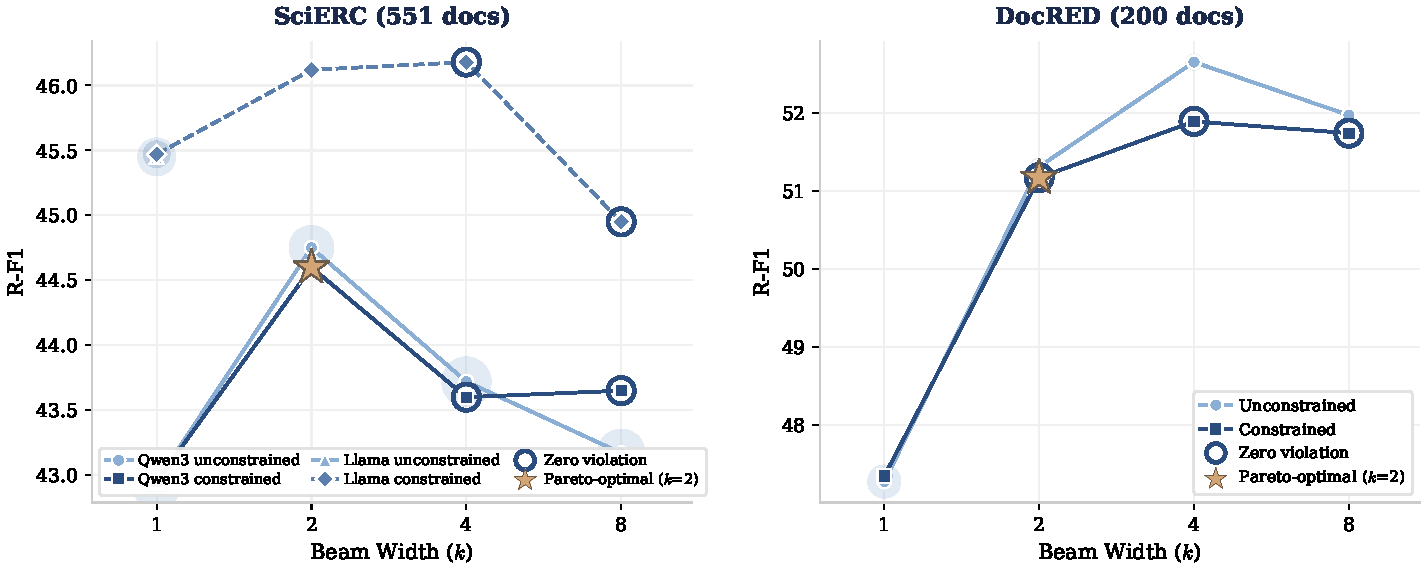
\includegraphics[width=\textwidth]{figures/beam_pareto.pdf}
\caption{Beam width vs.\ R-F1 under LoRA fine-tuning. Left: SciERC (Qwen3-8B solid, Llama-3.1-8B dashed; 551 docs). Right: DocRED (Llama-3.1-8B, 200 docs). Bubble area $\propto$ total violation rate (DR+CF+RV); rings mark zero-violation configurations. Star: Pareto-optimal ($k{=}2$).}
\label{fig:beam-pareto}
\end{figure*}

\begin{table}[h]
\centering
\small
\caption{Beam width sweep on SciERC (Qwen3-8B LoRA, 551 documents). \textsc{unc}: unconstrained; \textsc{con}: schema-constrained. Latency relative to $k{=}1$ unconstrained. Highlighted row: Pareto-optimal configuration.}
\label{tab:beam-sweep}
\resizebox{\columnwidth}{!}{%
\begin{tabular}{@{}cl cccc cc@{}}
\toprule
$k$ & Mode & E-F1 & R-F1 & DR (\%) & CF (\%) & Latency (s) & Rel.\ Lat. \\
\midrule
\multirow{2}{*}{1}
 & \textsc{unc} & 66.88 & 42.95 & 2.11 & 0    & 2.494 & 1.00$\times$ \\
 & \textsc{con} & 66.88 & 42.95 & \textbf{0} & 0.50 & 2.932 & 1.18$\times$ \\
\midrule
\multirow{2}{*}{2}
 & \textsc{unc} & 67.79 & 44.75 & 1.54 & 0    & 2.954 & 1.18$\times$ \\
 & \cellcolor{blue!8}\textsc{con} & \cellcolor{blue!8}67.71 & \cellcolor{blue!8}\textbf{44.60} & \cellcolor{blue!8}\textbf{0} & \cellcolor{blue!8}0.11 & \cellcolor{blue!8}3.463 & \cellcolor{blue!8}1.39$\times$ \\
\midrule
\multirow{2}{*}{4}
 & \textsc{unc} & 67.49 & 43.72 & 1.89 & 0    & 3.485 & 1.40$\times$ \\
 & \textsc{con} & 67.22 & 43.60 & \textbf{0} & 0    & 4.069 & 1.63$\times$ \\
\midrule
\multirow{2}{*}{8}
 & \textsc{unc} & 66.40 & 43.17 & 1.77 & 0    & 4.194 & 1.68$\times$ \\
 & \textsc{con} & 66.36 & 43.65 & \textbf{0} & 0    & 5.058 & 2.03$\times$ \\
\bottomrule
\end{tabular}}
\end{table}

\paragraph{Composability with fine-tuning.}
Under greedy decoding, the fine-tuned Qwen3-8B (LoRA, SciERC) with S1 constraints already achieves DR=0\% but retains CF=1.18\% (22 cross-field violations across 551 documents), with E-F1=67.05 and R-F1=43.77.
Adding beam search ($k{=}4$) eliminates all residual CF violations (1.18\%\,$\to$\,0\%), yielding zero violations across all four metrics (ET=0\%, RV=0\%, DR=0\%, CF=0\%) while preserving extraction quality (E-F1=66.88, R-F1=43.60; changes within $\pm$0.5\,pp).
Llama-3.1-8B (LoRA, SciERC) with S1 constraints and beam search ($k{=}4$) likewise achieves zero violations across all four metrics (ET=0\%, RV=0\%, DR=0\%, CF=0\%) with R-F1=46.18; the zero-violation result thus generalizes across calibrated model families.
The three constraint mechanisms (grammar masking, semantic domain-range filtering, and beam exploration) are thus fully composable: each addresses a distinct violation source without interfering with the others or degrading task performance.

The initial 50-document DocRED subset (Table~\ref{tab:beam-search}) was subsequently validated on the full 998-document set (Table~\ref{tab:beam-docred-998-zs}): both models achieve DR${=}$0\%, confirming subset representativeness.
Llama shows the larger improvement (CF 8.54\%\,$\to$\,1.00\%, 88\% reduction; R-F1 $+$2.6\,pp), consistent with beam search resolving constraint-search failures that greedy decoding cannot.

\begin{table}[h]
\centering
\small
\caption{Zero-shot beam search ($k{=}4$) under S1 constraints on the full DocRED dev set (998 documents).
ET/RV/DR/CF: violation rates (\%); PF: parse failure rate (\%); F1 $\times$100.}
\label{tab:beam-docred-998-zs}
\begin{tabular}{@{}lcccccc@{}}
\toprule
\textbf{Model} & ET & RV & DR$\,\downarrow$ & CF$\,\downarrow$ & E-F1$\,\uparrow$ & R-F1$\,\uparrow$ \\
\midrule
Qwen3-8B  & 0 & 0 & \textbf{0} & 4.94 & 58.19 & 8.72 \\
Llama-3.1-8B & 0 & 0 & \textbf{0} & 1.00 & 57.81 & 8.83 \\
\bottomrule
\end{tabular}
\end{table}

Table~\ref{tab:beam-docred-lora} reports LoRA + beam-4 results on the full DocRED dev set (998 documents), extending the fine-tuning composability evaluation from SciERC to the higher-$\bar{\kappa}$ regime.
Parse failure rates under LoRA beam-4 range from 1.3\% to 2.9\%, lower than the zero-shot rate.

\begin{table}[h]
\centering
\small
\caption{LoRA greedy vs.\ beam search ($k{=}4$) on DocRED (998 dev documents) under S1 constraints.
DR = domain/range, CF = cross-field violation rates (\%); PF = parse failure rate (\%); F1 $\times$ 100. ET and RV are 0\% in all rows.}
\label{tab:beam-docred-lora}
\resizebox{\columnwidth}{!}{%
\begin{tabular}{@{}llccccc@{}}
\toprule
\textbf{Model} & \textbf{Decoding} & DR$\,\downarrow$ & CF$\,\downarrow$ & E-F1$\,\uparrow$ & R-F1$\,\uparrow$ & PF \\
\midrule
\multirow{2}{*}{Qwen3-8B}
  & Greedy  & 0.01 & 0.41 & 81.43 & 40.56 & 8.52 \\
  & Beam-4  & \textbf{0} & 0.01 & 84.00 & 44.46 & 2.9 \\
\midrule
\multirow{2}{*}{Llama-3.1-8B}
  & Greedy  & 0.21 & 0.21 & 83.94 & 43.78 & 2.51 \\
  & Beam-4  & 0 & \textbf{0} & \textbf{85.23} & \textbf{47.17} & \textbf{1.3} \\
\bottomrule
\end{tabular}}
\end{table}

Llama-3.1-8B achieves zero violations across all four metrics (ET, RV, DR, CF = 0\%) on DocRED with LoRA + beam-4, extending the zero-violation result from SciERC to the high-$\bar{\kappa}$ regime.
Qwen3-8B achieves DR=0\% with near-zero CF (0.01\%); R-F1 is preserved ($\pm$0.06\,pp).
Combined with the sampling robustness results (Appendix~\ref{app:sampling}), these findings confirm that OntoCoDec's constraint enforcement is compatible with greedy, sampling, and beam search decoding without modification to the core constraint logic.

\paragraph{Latency overhead.}
Table~\ref{tab:beam-latency} reports wall-clock latency for greedy and beam search ($k{=}4$) under LoRA fine-tuning.

\begin{table}[h]
\centering
\small
\begin{tabular}{@{}lrr@{}}
\toprule
\textbf{Condition} & \textbf{s/doc} & \textbf{Overhead} \\
\midrule
Greedy unconstrained   & 2.612 & 1.00$\times$ \\
Greedy constrained (S1)& 2.873 & 1.10$\times$ \\
Beam-4 unconstrained   & 3.446 & 1.32$\times$ \\
Beam-4 constrained (S1)& 4.013 & 1.54$\times$ \\
\bottomrule
\end{tabular}
\caption{Latency per document (SciERC, 551 docs, Qwen3-8B LoRA FT, RTX PRO 6000 Blackwell). Overhead relative to greedy unconstrained.}
\label{tab:beam-latency}
\end{table}

Beam search itself adds 32\% latency (4 beams); constraint overhead increases from 10\% (greedy) to 17\% (beam) because each beam independently maintains grammar and semantic state.
Per-beam entity registry memory is $O(|\text{entities}|)$ per beam; at $k{=}8$ with typical document sizes, overhead is ${<}$1\,MB per beam, negligible relative to model memory.
The total 1.54$\times$ overhead is acceptable for offline batch IE; \texttt{early\_stopping} limits additional compute to partial-sequence exploration.

We also explored a type-consensus constraint that forces identical entity types across all relations within a document.
However, CF violations occur precisely where the consensus type conflicts with domain-range constraints, creating a fundamental CF$\leftrightarrow$DR trade-off.
With DR-aware enforcement (skipping consensus when it would violate domain-range), the layer becomes a no-op (100\% skip rate on 551 SciERC documents and 50 DocRED documents).
This confirms that beam search resolves the CF$\leftrightarrow$DR tension through a fundamentally different mechanism: token-level exploration of paths satisfying both constraints simultaneously.

\paragraph{TCR reranking under beam search.}
TCR reranking with beam search ($k{=}4$) showed no effect on either Qwen3-8B or Llama-3.1-8B under LoRA (0/551 SciERC candidates changed): fine-tuned beam candidates are already type-consistent (TCR score${=}$1.0 for all candidates), confirming that beam search implicitly subsumes post-hoc type consensus under fine-tuning.
This further strengthens the beam search deployment recommendation: beam achieves near-zero violations across all four types and renders post-hoc CF resolution unnecessary.

\section{Reproducibility Details}
\label{app:reproducibility}

\paragraph{Fine-tuning configuration.}
All four fine-tuned models (Qwen3-8B and Llama-3.1-8B-Instruct on SciERC and DocRED) use identical LoRA hyperparameters: rank $r{=}16$, $\alpha{=}32$, dropout $0.05$, no bias, targeting all attention and MLP projection layers (\texttt{q\_proj}, \texttt{k\_proj}, \texttt{v\_proj}, \texttt{o\_proj}, \texttt{gate\_proj}, \texttt{up\_proj}, \texttt{down\_proj}).
Training uses AdamW with learning rate $2{\times}10^{-4}$, cosine schedule, warmup ratio $0.1$, effective batch size $16$, bf16 precision, gradient checkpointing, and completion-only loss for 3 epochs.
SciERC trains on 1,762 examples (260 dev) for 333 steps; DocRED trains on 3,053 examples (998 dev) for 573 steps.
Maximum sequence length is 2,048 (SciERC) and 4,096 (DocRED).
All runs use seed 42.

\paragraph{Hardware and software.}
Training runs on a single NVIDIA RTX PRO 6000 Blackwell Server Edition GPU (98\,GB video RAM (VRAM)).
SciERC fine-tuning takes approximately 11 minutes per model; DocRED takes approximately 1.5 hours.
Software versions: PyTorch 2.10, Transformers 4.57, PEFT 0.19, TRL 1.1, Accelerate 1.13.

\paragraph{Inference time.}
Inference timing is reported in Appendix~\ref{app:runtime} (NVIDIA RTX PRO 6000 Blackwell Server Edition GPU, same hardware as training).
S1 constrained decoding adds $+$13.1\% wall-clock overhead on SciERC (Qwen3-8B, zero-shot greedy), lower on DocRED due to amortization over longer sequences; under LoRA fine-tuning, overhead is $+$10.0\% on SciERC.

\paragraph{Greedy decoding determinism.}
\label{app:greedy-determinism}
All main results use greedy decoding (temperature$\,{=}\,$0, argmax token selection).
Argmax is deterministic: the random seed controls \texttt{torch.manual\_seed} for sampling and dropout, neither of which is active during greedy inference.
We verify this with three seeds (42, 123, 456) across two LoRA fine-tuned models on all 551 SciERC documents.
Seeds 123 and 456, evaluated on the same GPU, produce byte-identical outputs for both Qwen3-8B and Llama-3.1-8B.
The residual variance in Table~\ref{tab:seed-variance} stems entirely from cross-hardware floating-point divergence: seed 42 was evaluated on a different server with a different CUDA driver version.
Even under this conservative upper bound, $\sigma(\text{E-F1}) \leq 0.16$\,pp, $\sigma(\text{R-F1}) \leq 0.43$\,pp, and $\sigma(\text{DR\%}) \leq 0.08$\,pp.
The constrained decoding DR\% reduction ($-$2.06\,pp for Qwen, $-$1.01\,pp for Llama) exceeds this variance by ${>}12\times$ (signal-to-noise ratio ${>}$\,12), confirming that observed improvements reflect genuine method effects rather than run-to-run noise.
We therefore report single-run results without error bars; bootstrap confidence intervals (10{,}000 iterations) are provided for F1 metrics.

\begin{table}[h]
\centering
\caption{Cross-seed variance for LoRA fine-tuned models on SciERC (551 documents, greedy decoding, seeds 42/123/456). Values: mean $\pm$ population $\sigma$ across three seeds. Seeds 123 and 456 produce identical outputs on the same GPU; all observed $\sigma$ reflects cross-server floating-point divergence.}
\label{tab:seed-variance}
\small
\resizebox{\columnwidth}{!}{%
\begin{tabular}{@{}lllccc@{}}
\toprule
Model & Dataset & Mode & E-F1 & R-F1 & DR\% \\
\midrule
Qwen3-8B & SciERC & Unc & $66.94 \pm 0.08$ & $43.25 \pm 0.43$ & $2.06 \pm 0.08$ \\
Qwen3-8B & SciERC & Con & $66.94 \pm 0.08$ & $43.22 \pm 0.39$ & $0.00 \pm 0.00$ \\
Llama-3.1-8B & SciERC & Unc & $67.99 \pm 0.16$ & $45.38 \pm 0.05$ & $1.04 \pm 0.05$ \\
Llama-3.1-8B & SciERC & Con & $67.99 \pm 0.16$ & $45.40 \pm 0.05$ & $0.03 \pm 0.04$ \\
\bottomrule
\end{tabular}}
\end{table}

\paragraph{Beam search non-determinism.}
Greedy decoding is deterministic (\S\ref{app:greedy-determinism} above).
Beam search ($k{\geq}2$) introduces non-determinism from GPU floating-point accumulation order; we report single-run results.
Based on the greedy cross-hardware variance ($\sigma < 0.5$\,pp, Table~\ref{tab:seed-variance}), beam search variance is expected to be of similar magnitude.

\paragraph{200-document subset justification.}
\label{app:power-analysis}
The 70B LoRA evaluation on DocRED uses a 200-document subset (vs.\ the full 998-document dev set used for 8B models).
To verify that this subset provides sufficient statistical power, we conduct a bootstrap analysis using the full 998-document 8B LoRA results as a reference population.
Resampling 200 documents 5{,}000 times yields a relation F1 margin of error of $\pm$3.3 points (95\% CI) and a DR violation rate margin of error of $\pm$0.45 percentage points---precise enough to support our conclusions.
For zero-shot models, where DR violations are prevalent (15.0\% unconstrained), a 200-document subset achieves 100\% power to detect the constrained decoding effect (Cohen's $h = 0.80$); for fine-tuned models, where violations are already rare ($<$0.5\%), 94.9\% of 200-document subsamples correctly identify the direction of DR reduction, and the primary effect is established on the full 998-document evaluation.

% Appendix: Statistical Power Analysis for WikiEvents n=20
% Addresses reviewer concern about WikiEvents FT statistical power.
% Include via % Appendix: Statistical Power Analysis for WikiEvents n=20
% Addresses reviewer concern about WikiEvents FT statistical power.
% Include via % Appendix: Statistical Power Analysis for WikiEvents n=20
% Addresses reviewer concern about WikiEvents FT statistical power.
% Include via \input{appendix_power_analysis} in the appendix.

\paragraph{Statistical power across evaluation settings.}
\label{app:power-analysis-full}
Table~\ref{tab:power-analysis} reports bootstrap confidence interval width and minimum detectable effect (MDE) for F1 across evaluation settings (${\geq}$1{,}000 bootstrap resamples; MDE at 80\% power, $\alpha{=}0.05$, paired test, $\rho{=}0.9$).

\begin{table}[h]
\centering
\small
\begin{tabular}{lrrr}
\toprule
\textbf{Dataset} & \textbf{$n$} & \textbf{95\% CI (F1)} & \textbf{MDE (F1)} \\
\midrule
SciERC & 551 & $\pm$1.8\,pp & 1.2\,pp \\
DocRED & 998 & $\pm$0.8\,pp & 0.5\,pp \\
DocRED (70B) & 200 & $\pm$3.3\,pp & 2.1\,pp \\
WikiEvents & 20 & $\pm$3.0\,pp & 2.0\,pp \\
\bottomrule
\end{tabular}
\caption{Statistical precision by dataset size.
95\% CI: bootstrap confidence interval half-width for per-configuration F1.
MDE: minimum detectable F1 difference at 80\% power ($\alpha{=}0.05$, paired test, conservative $\rho{=}0.9$).
SciERC/DocRED: zero-shot Rel-F1; DocRED (70B): LoRA Rel-F1 (200-doc subset); WikiEvents: LoRA Arg-F1.}
\label{tab:power-analysis}
\end{table}

WikiEvents' $n{=}20$ yields an Arg-F1 margin of error of $\pm$3.0\,pp---comparable to the 200-document DocRED subset ($\pm$3.3\,pp)---with MDE${\approx}$2.0\,pp.
However, the primary WikiEvents claims concern violation elimination, not F1 improvement: RoV drops from 8.8--38.3\% to exactly 0\% across both models (bootstrap 95\% CI $[0\%,\,0\%]$ vs.\ $[2.4\%,\,15.4\%]$ / $[25.4\%,\,46.7\%]$; power${\approx}$1.0).
The small test set limits detection of subtle F1 shifts, but complete elimination of schema violations is unambiguous at $n{=}20$; the primary evidence for F1 preservation rests on SciERC ($n{=}551$) and DocRED ($n{=}998$), where CIs are ${\leq}$1.8\,pp.
 in the appendix.

\paragraph{Statistical power across evaluation settings.}
\label{app:power-analysis-full}
Table~\ref{tab:power-analysis} reports bootstrap confidence interval width and minimum detectable effect (MDE) for F1 across evaluation settings (${\geq}$1{,}000 bootstrap resamples; MDE at 80\% power, $\alpha{=}0.05$, paired test, $\rho{=}0.9$).

\begin{table}[h]
\centering
\small
\begin{tabular}{lrrr}
\toprule
\textbf{Dataset} & \textbf{$n$} & \textbf{95\% CI (F1)} & \textbf{MDE (F1)} \\
\midrule
SciERC & 551 & $\pm$1.8\,pp & 1.2\,pp \\
DocRED & 998 & $\pm$0.8\,pp & 0.5\,pp \\
DocRED (70B) & 200 & $\pm$3.3\,pp & 2.1\,pp \\
WikiEvents & 20 & $\pm$3.0\,pp & 2.0\,pp \\
\bottomrule
\end{tabular}
\caption{Statistical precision by dataset size.
95\% CI: bootstrap confidence interval half-width for per-configuration F1.
MDE: minimum detectable F1 difference at 80\% power ($\alpha{=}0.05$, paired test, conservative $\rho{=}0.9$).
SciERC/DocRED: zero-shot Rel-F1; DocRED (70B): LoRA Rel-F1 (200-doc subset); WikiEvents: LoRA Arg-F1.}
\label{tab:power-analysis}
\end{table}

WikiEvents' $n{=}20$ yields an Arg-F1 margin of error of $\pm$3.0\,pp---comparable to the 200-document DocRED subset ($\pm$3.3\,pp)---with MDE${\approx}$2.0\,pp.
However, the primary WikiEvents claims concern violation elimination, not F1 improvement: RoV drops from 8.8--38.3\% to exactly 0\% across both models (bootstrap 95\% CI $[0\%,\,0\%]$ vs.\ $[2.4\%,\,15.4\%]$ / $[25.4\%,\,46.7\%]$; power${\approx}$1.0).
The small test set limits detection of subtle F1 shifts, but complete elimination of schema violations is unambiguous at $n{=}20$; the primary evidence for F1 preservation rests on SciERC ($n{=}551$) and DocRED ($n{=}998$), where CIs are ${\leq}$1.8\,pp.
 in the appendix.

\paragraph{Statistical power across evaluation settings.}
\label{app:power-analysis-full}
Table~\ref{tab:power-analysis} reports bootstrap confidence interval width and minimum detectable effect (MDE) for F1 across evaluation settings (${\geq}$1{,}000 bootstrap resamples; MDE at 80\% power, $\alpha{=}0.05$, paired test, $\rho{=}0.9$).

\begin{table}[h]
\centering
\small
\begin{tabular}{lrrr}
\toprule
\textbf{Dataset} & \textbf{$n$} & \textbf{95\% CI (F1)} & \textbf{MDE (F1)} \\
\midrule
SciERC & 551 & $\pm$1.8\,pp & 1.2\,pp \\
DocRED & 998 & $\pm$0.8\,pp & 0.5\,pp \\
DocRED (70B) & 200 & $\pm$3.3\,pp & 2.1\,pp \\
WikiEvents & 20 & $\pm$3.0\,pp & 2.0\,pp \\
\bottomrule
\end{tabular}
\caption{Statistical precision by dataset size.
95\% CI: bootstrap confidence interval half-width for per-configuration F1.
MDE: minimum detectable F1 difference at 80\% power ($\alpha{=}0.05$, paired test, conservative $\rho{=}0.9$).
SciERC/DocRED: zero-shot Rel-F1; DocRED (70B): LoRA Rel-F1 (200-doc subset); WikiEvents: LoRA Arg-F1.}
\label{tab:power-analysis}
\end{table}

WikiEvents' $n{=}20$ yields an Arg-F1 margin of error of $\pm$3.0\,pp---comparable to the 200-document DocRED subset ($\pm$3.3\,pp)---with MDE${\approx}$2.0\,pp.
However, the primary WikiEvents claims concern violation elimination, not F1 improvement: RoV drops from 8.8--38.3\% to exactly 0\% across both models (bootstrap 95\% CI $[0\%,\,0\%]$ vs.\ $[2.4\%,\,15.4\%]$ / $[25.4\%,\,46.7\%]$; power${\approx}$1.0).
The small test set limits detection of subtle F1 shifts, but complete elimination of schema violations is unambiguous at $n{=}20$; the primary evidence for F1 preservation rests on SciERC ($n{=}551$) and DocRED ($n{=}998$), where CIs are ${\leq}$1.8\,pp.

\section{Effect of Document Length on Constraint Effectiveness}
\label{app:doc-length}

To examine whether OntoCoDec's constraint effectiveness varies with document complexity, we partition test documents into three length bins (tertile split by word count) and report per-bin violation counts and F1.

\begin{table}[h]
\centering
\small
\caption{Document length breakdown on SciERC (Qwen3-8B). Tertile boundaries: Short $\leq$ 19 words, Medium $\leq$ 27, Long $>$ 27.}
\label{tab:doc-length-scierc}
\resizebox{\columnwidth}{!}{%
\begin{tabular}{ll rrrrr rr}
\toprule
\textbf{Bin} & \textbf{Mode} & \textbf{ET} & \textbf{RV} & \textbf{DR} & \textbf{CF} & \textbf{Total} & \textbf{E-F1} & \textbf{R-F1} \\
\midrule
Short (196)  & Uncon. &  1 &  5 &  57 & 0 &  63 & 32.4 &  8.9 \\
             & Const. &  0 &  0 &   5 & 5 &  10 & 32.4 &  8.9 \\
\midrule
Medium (180) & Uncon. &  6 &  9 & 104 & 0 & 119 & 27.8 &  6.7 \\
             & Const. &  0 &  0 &   7 & 15 & 22 & 27.8 &  6.7 \\
\midrule
Long (175)   & Uncon. &  3 & 10 & 104 & 1 & 118 & 29.9 &  7.0 \\
             & Const. &  0 &  0 &   4 & 20 & 24 & 30.0 &  7.3 \\
\bottomrule
\end{tabular}}
\end{table}

\begin{table}[h]
\centering
\small
\caption{Document length breakdown on DocRED (Qwen3-8B). Tertile boundaries: Short $\leq$ 160 words, Medium $\leq$ 208, Long $>$ 208.}
\label{tab:doc-length-docred}
\resizebox{\columnwidth}{!}{%
\begin{tabular}{ll rrrrr rr}
\toprule
\textbf{Bin} & \textbf{Mode} & \textbf{ET} & \textbf{RV} & \textbf{DR} & \textbf{CF} & \textbf{Total} & \textbf{E-F1} & \textbf{R-F1} \\
\midrule
Short (336)  & Uncon. & 177 & 1238 & 1021 &   9 & 2445 & 61.1 &  9.3 \\
             & Const. &   0 &    0 &  495 & 138 &  633 & 62.6 &  9.6 \\
\midrule
Medium (332) & Uncon. & 147 & 1742 & 1047 &   5 & 2941 & 59.3 &  7.9 \\
             & Const. &   0 &    5 &  544 & 180 &  729 & 60.7 &  8.5 \\
\midrule
Long (330)   & Uncon. & 176 & 2209 & 1162 &   3 & 3550 & 53.9 &  5.6 \\
             & Const. &   0 &    0 &  731 & 200 &  931 & 54.8 &  5.8 \\
\bottomrule
\end{tabular}}
\end{table}

\begin{table}[h]
\centering
\small
\caption{Violation reduction percentage by document length bin (Qwen3-8B, S1 constraints).}
\label{tab:doc-length-reduction}
\resizebox{\columnwidth}{!}{%
\begin{tabular}{l rr rr}
\toprule
& \multicolumn{2}{c}{\textbf{SciERC}} & \multicolumn{2}{c}{\textbf{DocRED}} \\
\cmidrule(lr){2-3} \cmidrule(lr){4-5}
\textbf{Bin} & \textbf{Viols (U$\to$C)} & \textbf{Red.\%} & \textbf{Viols (U$\to$C)} & \textbf{Red.\%} \\
\midrule
Short  & 63 $\to$ 10  & 84.1 & 2445 $\to$ 633  & 74.1 \\
Medium & 119 $\to$ 22 & 81.5 & 2941 $\to$ 729  & 75.2 \\
Long   & 118 $\to$ 24 & 79.7 & 3550 $\to$ 931  & 73.8 \\
\bottomrule
\end{tabular}}
\end{table}

The violation reduction rate is consistent across all length bins: 80--84\% for SciERC and 74--75\% for DocRED.
Longer documents produce more violations in the unconstrained setting (e.g., DocRED long-bin: 3,550 vs.\ short-bin: 2,445), yet OntoCoDec achieves proportionally similar reduction; the constraint framework scales reliably with document complexity.
ET and RV violations are fully eliminated across all bins.
F1 scores are preserved or slightly improved under constrained decoding, with DocRED showing +0.9--1.5 E-F1 and +0.2--0.6 R-F1 improvement in the constrained setting.

\section{Prompt Sensitivity Analysis}
\label{app:prompt-sensitivity}

To verify that OntoCoDec's constraint enforcement is robust to prompt variation, we evaluate three prompt variants on SciERC using Qwen3-8B (551 test documents): \textbf{Default} (the prompt used in all main experiments), \textbf{Minimal} (a shortened version listing only entity/relation types), and \textbf{Detailed} (an extended version with type definitions and extraction guidelines). All three variants share the same output JSON schema; only the instruction text differs. Each variant is decoded in both unconstrained and constrained (full Stage~1) modes.

\begin{table}[h]
\centering
\small
\caption{Prompt sensitivity results on SciERC (551 documents). Top: Qwen3-8B; bottom: Llama-3.1-70B (AWQ INT4). ET, RV, DR denote entity-type, relation-vocabulary, and domain-range violation rates (\%), respectively. $\Delta$DR shows the relative reduction from unconstrained to constrained decoding.}
\label{tab:prompt-sensitivity}
\resizebox{\columnwidth}{!}{%
\begin{tabular}{llcccccc}
\toprule
\textbf{Prompt} & \textbf{Mode} & \textbf{ET\%} & \textbf{RV\%} & \textbf{DR\%} & \textbf{$\Delta$DR} & \textbf{E-F1} & \textbf{R-F1} \\
\midrule
\multirow{2}{*}{Default}
  & Unconstrained & 0.40 & 1.39 & 15.37 & \multirow{2}{*}{94.0\%} & 31.01 & 8.23 \\
  & Constrained   & 0.00 & 0.00 &  0.93 &                         & 30.98 & 8.36 \\
\midrule
\multirow{2}{*}{Minimal}
  & Unconstrained & 0.58 & 1.16 & 16.91 & \multirow{2}{*}{94.6\%} & 31.98 & 7.91 \\
  & Constrained   & 0.00 & 0.00 &  0.92 &                         & 31.99 & 7.85 \\
\midrule
\multirow{2}{*}{Detailed}
  & Unconstrained & 0.22 & 0.45 & 11.07 & \multirow{2}{*}{94.2\%} & 33.55 & 10.48 \\
  & Constrained   & 0.00 & 0.00 &  0.64 &                         & 33.56 & 10.48 \\
\midrule
\multicolumn{8}{l}{\textit{Llama-3.1-70B-Instruct (AWQ INT4)}} \\
\midrule
\multirow{2}{*}{Default}
  & Unconstrained & 0.00 & 0.61 & 6.41 & \multirow{2}{*}{100\%} & 35.22 & 11.23 \\
  & Constrained   & 0.00 & 0.00 & 0.00 &                        & 35.19 & 11.24 \\
\midrule
\multirow{2}{*}{Minimal}
  & Unconstrained & 0.27 & 5.88 & 0.22 & \multirow{2}{*}{100\%} & 37.51 & 13.42 \\
  & Constrained   & 0.00 & 0.00 & 0.00 &                        & 37.22 & 11.35 \\
\midrule
\multirow{2}{*}{Detailed}
  & Unconstrained & 0.00 & 0.26 & 4.57 & \multirow{2}{*}{100\%} & 40.42 & 11.12 \\
  & Constrained   & 0.00 & 0.00 & 0.00 &                        & 40.35 & 11.16 \\
\bottomrule
\end{tabular}}
\end{table}

Table~\ref{tab:prompt-sensitivity} shows that constrained decoding eliminates entity-type and relation-vocabulary violations entirely (ET and RV drop to 0\%) for all prompt variants at both scales. At 8B, domain-range violations are reduced by 94.0\%--94.6\% with a standard deviation of only 0.3\,pp across prompts; F1 scores remain effectively unchanged (max shift 0.13\,pp R-F1).

At 70B, constrained decoding achieves DR${=}$0\% across all three prompts ($\Delta$DR${=}$100\%), consistent with the scale-dependent semantic layer interaction observed in the main experiments (\S\ref{sec:70b-results}). Baseline DR varies widely (0.22\%--6.41\%), yet constrained decoding converges to zero in all cases; CF is introduced as expected (0.62\%--3.50\%), consistent with the per-triple enforcement trade-off.

Prompt variation has a measurable effect on baseline (unconstrained) violation rates at both scales: 8B DR ranges from 11.1\% (Detailed) to 16.9\% (Minimal); 70B from 0.22\% to 6.41\%. Under constrained decoding, this variance collapses, confirming that the mechanism is orthogonal to prompting and generalizes without prompt-specific tuning.

\paragraph{LoRA fine-tuned prompt invariance.}
Under LoRA fine-tuning at 70B, prompt invariance is preserved: Minimal and Detailed prompts both achieve DR${=}$0\% under S1, with CF at 0.62\% and 0.75\% respectively---consistent with the zero-shot 70B pattern above.
This confirms that OntoCoDec's constraint enforcement is robust to prompt variation across both zero-shot and fine-tuned regimes.

% Appendix — Error Analysis and Case Studies

\section{Error Analysis and Case Studies}
\label{app:case-studies}

\definecolor{violation}{RGB}{220,50,50}
\definecolor{fixed}{RGB}{34,139,34}
\definecolor{cfwarn}{RGB}{200,120,0}
\newcommand{\viol}[1]{\textcolor{violation}{\st{#1}}}
\newcommand{\fixd}[1]{\textcolor{fixed}{\textbf{#1}}}

We present four representative cases illustrating constraint behavior across violation types. Cases 1--3 demonstrate OntoCoDec's corrective mechanisms; Case 4 illustrates a limitation.

\subsection{Domain-Range Correction}
\label{app:case-dr}

\noindent\textbf{Input (SciERC, Qwen3-8B):} \textit{``We present a novel model-based approach to recover the shapes and the poses of transparent objects from known motion.''}

The unconstrained model assigns \textsc{OtherScientificTerm} to ``shapes'' and ``poses,'' producing \textsc{Feature-of}(\textsc{Task}, \textsc{OtherScientificTerm}) triples that violate domain/range constraints. The semantic layer redirects the tail type to \textsc{Task}, yielding schema-compliant triples (Table~\ref{tab:case1}).

\begin{table}[h]
\centering
\small
\caption{OntoCoDec corrects three Feature-of DR violations. \textcolor{violation}{Red}/\ding{55} = violation; \textcolor{fixed}{\textbf{green/bold}}/\ding{51} = corrected (shape markers provided for colorblind accessibility).}
\label{tab:case1}
\begin{tabular}{@{}p{3.2cm}lll@{}}
\toprule
\textbf{Triple} & \textbf{Head} & \textbf{Tail} & \textbf{DR} \\
\midrule
\multicolumn{4}{@{}l}{\textit{Unconstrained (3 violations)}} \\
\midrule
Feature-of(recover, shapes) & Task & \textcolor{violation}{OtherSciTerm} & \textcolor{violation}{\ding{55}} \\
Feature-of(recover, poses) & Task & \textcolor{violation}{OtherSciTerm} & \textcolor{violation}{\ding{55}} \\
Feature-of(recover, transp.\ obj.) & Task & \textcolor{violation}{OtherSciTerm} & \textcolor{violation}{\ding{55}} \\
Used-for(model approach, recover) & Method & Task & \ding{51} \\
\midrule
\multicolumn{4}{@{}l}{\textit{OntoCoDec (0 violations)}} \\
\midrule
Feature-of(recover, shapes) & Task & \textcolor{fixed}{Task} & \textcolor{fixed}{\ding{51}} \\
Feature-of(recover, poses) & Task & \textcolor{fixed}{Task} & \textcolor{fixed}{\ding{51}} \\
Used-for(model approach, recover) & Method & Task & \ding{51} \\
\bottomrule
\end{tabular}
\end{table}

\subsection{Dual-Layer Vocabulary and Type Correction}
\label{app:case-rv-dr}

\noindent\textbf{Input (DocRED, Qwen3-8B):} \textit{``Skai TV is a Greek free-to-air television network based in Piraeus. It is part of the Skai Group, one of the largest media groups in the country.''}

The unconstrained model generates natural-language relation names (e.g., ``country of origin'') instead of Wikidata P-codes, triggering RV violations. The grammar layer forces valid P-codes; the semantic layer ensures type compatibility (Table~\ref{tab:case2}).

\begin{table}[h]
\centering
\small
\caption{Layer~1 eliminates RV violations; Layer~2 corrects DR types on DocRED.}
\label{tab:case2}
\resizebox{\columnwidth}{!}{%
\begin{tabular}{@{}p{4.5cm}p{1.8cm}p{1.2cm}@{}}
\toprule
\textbf{Unconstrained Output} & \textbf{Violation} & \textbf{Type} \\
\midrule
rel=``country of origin'' & Not in schema & RV \\
rel=``headquarters location'' & Not in schema & RV \\
rel=``part of'' & Not in schema & RV \\
rel=``location of formation'' & Not in schema & RV \\
\midrule
\textbf{OntoCoDec Output} & & \\
\midrule
rel=P495 (Skai TV, Greece) & ORG$\to$LOC & \ding{51} \\
rel=P159 (Skai TV, Piraeus) & ORG$\to$LOC & \ding{51} \\
rel=P127 (Skai TV, Skai Group) & ORG$\to$ORG & \ding{51} \\
rel=P17 (Piraeus, Greece) & LOC$\to$LOC & \ding{51} \\
\bottomrule
\end{tabular}}
\end{table}

\subsection{Scale Effect on Schema Compliance}
\label{app:case-scale}

\noindent\textbf{Input (SciERC):} \textit{``This paper investigates the utility of applying standard MT evaluation methods (BLEU, NIST, WER and PER) to building classifiers to predict semantic equivalence and entailment.''}

Both Qwen3-8B and Llama-3.1-70B-Instruct (AWQ INT4) mistype ``MT evaluation methods'' as \textsc{Method} (gold: \textsc{Metric}), but the downstream constraint behavior differs (Table~\ref{tab:case3}). The 70B model produces fewer violations (2 vs.\ 4) and chooses a different relation (Part-of vs.\ Hyponym-of), yet OntoCoDec corrects both.

\begin{table}[h]
\centering
\small
\caption{8B vs.\ 70B on the same input. OntoCoDec corrects violations at both scales; CF arises when type corrections conflict with entity-list assignments.}
\label{tab:case3}
\resizebox{\columnwidth}{!}{%
\begin{tabular}{@{}llll@{}}
\toprule
\textbf{Setting} & \textbf{Relation} & \textbf{Types} & \textbf{DR} \\
\midrule
\multicolumn{4}{@{}l}{\textit{Qwen3-8B Unconstrained}} \\
Hyponym-of(MT eval, BLEU) & Meth$\to$\textcolor{violation}{Metric} & \textcolor{violation}{\ding{55}} \\
Hyponym-of(MT eval, NIST) & Meth$\to$\textcolor{violation}{Metric} & \textcolor{violation}{\ding{55}} \\
Hyponym-of(MT eval, WER) & Meth$\to$\textcolor{violation}{Metric} & \textcolor{violation}{\ding{55}} \\
Hyponym-of(MT eval, PER) & Meth$\to$\textcolor{violation}{Metric} & \textcolor{violation}{\ding{55}} \\
\midrule
\multicolumn{4}{@{}l}{\textit{Qwen3-8B OntoCoDec}} \\
Hyponym-of(MT eval, BLEU) & Meth$\to$\textcolor{fixed}{Meth} & \textcolor{fixed}{\ding{51}} \\
Hyponym-of(MT eval, NIST) & Meth$\to$\textcolor{fixed}{Meth} & \textcolor{fixed}{\ding{51}} \\
\multicolumn{3}{@{}l}{\textcolor{cfwarn}{CF: BLEU typed Metric in entity list, Method in relation}} \\
\midrule
\multicolumn{4}{@{}l}{\textit{Llama-3.1-70B Unconstrained}} \\
Part-of(BLEU, MT eval) & Metric$\to$\textcolor{violation}{Meth} & \textcolor{violation}{\ding{55}} \\
Part-of(NIST, MT eval) & Metric$\to$\textcolor{violation}{Meth} & \textcolor{violation}{\ding{55}} \\
\midrule
\multicolumn{4}{@{}l}{\textit{Llama-3.1-70B OntoCoDec}} \\
Part-of(BLEU, MT eval) & Metric$\to$\textcolor{fixed}{Generic} & \textcolor{fixed}{\ding{51}} \\
Part-of(NIST, MT eval) & Metric$\to$\textcolor{fixed}{Generic} & \textcolor{fixed}{\ding{51}} \\
\bottomrule
\end{tabular}}
\end{table}

\subsection{Limitation: Trajectory Divergence under Constraints}
\label{app:case-cf}

\noindent\textbf{Input (SciERC, Mistral-7B):} \textit{``Amorph recognizes NE items in two stages: dictionary lookup and rule application.''}

The gold annotation types ``Amorph'' as \textsc{Method} and ``NE items'' as \textsc{OtherScientificTerm}, with Used-for(Amorph, NE items). The unconstrained model mistypes ``Amorph'' but coincidentally produces the correct relation. Under OntoCoDec, modified token probabilities alter the generation trajectory entirely and produce a different (non-gold) relation (Table~\ref{tab:case4}). This illustrates a fundamental property of autoregressive generation under modified distributions: constraint enforcement can change the entire output path, not just individual token choices.

\begin{table}[h]
\centering
\small
\caption{Constrained decoding changes the generation trajectory. The unconstrained model coincidentally produced the gold triple despite type errors.}
\label{tab:case4}
\resizebox{\columnwidth}{!}{%
\begin{tabular}{@{}p{4.2cm}ll@{}}
\toprule
\textbf{Setting} & \textbf{Output} & \textbf{Gold?} \\
\midrule
\textbf{Gold} & Used-for(Amorph\textsuperscript{Meth}, NE items\textsuperscript{OtherSci}) & -- \\
\midrule
\textbf{Unconstr.} & Used-for(Amorph\textsuperscript{OtherSci}, NE items\textsuperscript{Task}) & \textcolor{fixed}{\ding{51}} \\
\midrule
\textbf{OntoCoDec} & Used-for(Amorph\textsuperscript{OtherSci}, recognizes\textsuperscript{Gen}) & \textcolor{violation}{\ding{55}} \\
 & Feature-of(NE items\textsuperscript{Task}, in two stages\textsuperscript{Gen}) & \textcolor{violation}{\ding{55}} \\
\bottomrule
\end{tabular}}
\end{table}

\subsection{Error Analysis: Constraint Impact on Prediction Quality}
\label{app:error-analysis}

We analyze errors from Qwen3-8B LoRA + S1 on SciERC (551 documents; R-F1 43.77, 460 TP, 668 FP, 514 FN) across three categories.

\paragraph{False negatives: constraint-blocked vs.\ model-limited.}
Of 514 false negatives, only one (0.2\%) is attributable to constraint enforcement:

\noindent\textit{fn\_001} (constraint-blocked): ``\textit{Experiments on the TREC Blog track test set show that both groups of credibility indicators significantly improve retrieval effectiveness.}'' \\
Gold: Evaluate-for(retrieval effectiveness\textsuperscript{Metric}, credibility indicators\textsuperscript{OtherSci}).
The unconstrained model generates this triple correctly, but under S1, conflicting type assignments to `credibility indicators' (OtherScientificTerm in entity list vs.\ Method in Evaluate-for's tail) trigger a CF violation, redirecting generation to a reversed Used-for triple.

\noindent\textit{fn\_004} (relation type confusion): ``\textit{Amorph recognizes NE items in two stages: dictionary lookup and rule application.}'' \\
Gold: Part-of(dictionary lookup\textsuperscript{Meth}, Amorph\textsuperscript{Meth}).
The model predicts Used-for instead of Part-of---both are schema-valid for Method$\to$Method pairs, so constraints provide no corrective signal. This Part-of$\leftrightarrow$Used-for confusion is the dominant FN pattern.

\paragraph{False positives: schema-valid but incorrect.}

\noindent\textit{fp\_001} (wrong relation type): Same sentence as fn\_004. The model generates Used-for(dictionary lookup, Amorph) where gold is Part-of. Used-for is the majority relation in SciERC (56\% of all relations), causing systematic over-prediction. Since both relation types are schema-valid for the entity type pair, constraints cannot distinguish them.

\noindent\textit{fp\_007} (hallucinated relation): ``\textit{The classifiers show little gain from information about meeting context.}'' \\
No gold relation exists. The model generates Used-for(meeting context\textsuperscript{OtherSci}, classifiers\textsuperscript{Meth}), ignoring the negation in ``show little gain from.'' The instrumental preposition ``from'' triggers relation generation despite the negative result.

\paragraph{CF violations: entity type polysemy.}

\noindent\textit{cf\_001} (Generic$\leftrightarrow$Method): ``\textit{A basic reason behind this is that the overall approach extends the approach described in a companion paper\ldots}'' \\
The entity `approach' receives Generic in one Used-for relation and Method in another. The gold type is Generic; the polysemy of `approach' (generic reference vs.\ specific method) causes per-relation type assignment to diverge.

\noindent\textit{cf\_005} (Material$\leftrightarrow$Task): ``\textit{Experimental evaluations on two challenging person re-identification datasets demonstrate the superiority of the proposed model\ldots}'' \\
The compound noun `person re-identification datasets' contains both a task component and a data component. The model assigns Material in one Evaluate-for relation and Task in another within the same sentence.

\paragraph{Summary.}
Structural constraints eliminate type-invalid outputs (DR$\leq$0.21\%), but semantic ambiguity within schema-valid space---relation type confusion, entity type polysemy---remains the dominant error source. Only 1 of 514 false negatives (0.2\%) was attributable to constraint enforcement, confirming that the recall cost of type constraints is negligible.

\paragraph{Downstream impact of violation removal.}
\label{app:downstream-impact}

A natural concern with schema-constrained decoding is whether enforcing ontological validity removes \emph{lucky violations}---predictions that happen to be correct (true positives) yet violate the schema.
To quantify this trade-off, we audit all true-positive relation triples produced by unconstrained fine-tuned models and check whether any of them carry a domain--range (DR) violation, i.e., an entity-type pair \mbox{$\langle h_\tau, t_\tau \rangle$} not sanctioned by the ontology for that relation.

\begin{table}[h]
\centering
\small
\begin{tabular}{llrrrl}
\toprule
\textbf{Dataset} & \textbf{Model} & \textbf{TP} & \textbf{Lucky} & \textbf{\%\,TP} & \textbf{R drop} \\
\midrule
SciERC & Qwen-LoRA  & 461  & 4 & 0.87\% & 0.41\,pp \\
SciERC & Llama-LoRA & 467  & 5 & 1.07\% & 0.51\,pp \\
DocRED & Qwen-LoRA  & 5746 & 1 & 0.02\% & 0.01\,pp \\
DocRED & Llama-LoRA & 6226 & 1 & 0.02\% & 0.01\,pp \\
\bottomrule
\end{tabular}
\caption{Lucky violations: true-positive triples that carry a domain--range violation. \textbf{Lucky} counts such triples; \textbf{R drop} is the recall decrease (in percentage points) if they were removed.}
\label{tab:lucky-violations-detail}
\end{table}

Across all four configurations, lucky violations account for at most 1.07\% of true positives (5 out of 467 on SciERC with Llama-LoRA) and as few as 0.02\% on DocRED.
The corresponding recall drop is negligible---at most 0.51 percentage points---while the vast majority of violated triples that constraints remove are false positives.
For example, on DocRED with Qwen-LoRA, constraints eliminate 164 schema-violating predictions but only 1 of them is actually correct; the other 163 are errors that would pollute a downstream knowledge graph.

Inspecting the lucky violations qualitatively, they arise from borderline entity-type assignments rather than genuine schema gaps.
On SciERC, the recurring pattern involves \textsc{Metric}-typed entities (e.g., BLEU, NIST) appearing as heads of \texttt{Hyponym-of} relations, a pair absent from the training ontology because these metrics are rarely annotated as hyponyms.
On DocRED, the single lucky violation stems from an entity typed as \textsc{Misc} instead of \textsc{Org} (``Assassin's Creed Unity''), making its \texttt{developer} relation invalid under the schema despite being factually correct.

These findings confirm that schema-constrained decoding introduces a minimal recall cost while providing a substantial precision gain.
Retaining these few lucky violations would allow schema-invalid triples into the knowledge graph, undermining the structural guarantees that motivate constrained decoding in the first place.
The net effect is overwhelmingly positive: constraints act as a high-precision filter that removes far more erroneous triples than correct ones.

\section{Ontology Scalability}
\label{app:scalability}

\begin{table}[h]
\centering
\small
\resizebox{\columnwidth}{!}{%
\begin{tabular}{@{}lrrrr@{}}
\toprule
\textbf{Scale} & \textbf{Types} & \textbf{Rels} & \textbf{Compile (s)} & \textbf{Overhead} \\
\midrule
Small (SciERC) & 6 & 7 & 0.33 & 1.02$\times$ \\
Medium (DocRED) & 6 & 96 & 0.32 & 1.03$\times$ \\
Large (synth.) & 100 & 500 & 0.35 & 1.03$\times$ \\
XLarge (synth.) & 200 & 1{,}000 & 0.42 & 1.03$\times$ \\
\bottomrule
\end{tabular}}
\caption{Compilation time (one-time) and per-token inference overhead across ontology scales. Small and Medium use real ontologies; Large and XLarge use synthetic ontologies with random domain/range constraints. Overhead measured on Qwen3-8B, 10 documents per scale.}
\label{tab:scalability}
\end{table}

Full constraint compilation (schema parsing + grammar build) scales sub-linearly (0.32\,s to 0.42\,s for 7$\to$1{,}000 relations; Table~\ref{tab:scalability}); within this, the XGrammar automaton accounts for $\sim$0.044\,s and semantic constraint compilation grows linearly but remains negligible (0.4\,ms to 17\,ms).
Inference overhead is constant at 2--3\% because XGrammar uses precompiled bitmasks ($O(1)$ per token) and the semantic layer checks only the active relation's domain/range set rather than the full ontology.
The practical limit is first-token uniqueness: when entity types exceed $\sim$200, prefix collisions in the tokenizer vocabulary may require fallback to multi-token disambiguation (\S\ref{sec:dynamic-masking}).

\section{Full Fine-Tuning Baseline}
\label{app:full-ft}

To verify that constraint effectiveness generalizes beyond LoRA, we evaluate Qwen3-8B with full-parameter fine-tuning on SciERC (same data, 3 epochs, lr=$2{\times}10^{-4}$, seed 42).

\begin{table}[h]
\centering
\small
\begin{tabular}{@{}lrrrr@{}}
\toprule
& \textbf{E-F1} & \textbf{R-F1} & \textbf{DR\%} & \textbf{CF\%} \\
\midrule
Full FT unconstrained & 64.78 & 37.89 & 2.74 & 0 \\
Full FT + S1 & 64.78 & 37.89 & \textbf{0} & 1.31 \\
\midrule
LoRA unconstrained & 67.05 & 43.86 & 1.95 & 0 \\
LoRA + S1 & 67.05 & 43.77 & \textbf{0} & 1.18 \\
\bottomrule
\end{tabular}
\caption{Full fine-tuning vs.\ LoRA on SciERC (Qwen3-8B, 551 docs). Constraints eliminate DR under both methods. Full FT underperforms LoRA, likely due to an untuned learning rate ($2{\times}10^{-4}$, standard for LoRA but high for full FT). F1 is unaffected by constraints in both cases.}
\label{tab:full-ft}
\end{table}

Full fine-tuning retains 2.74\% DR violations (30 triples), concentrated in Part-of (14.6\%), Hyponym-of (9.6\%), and Evaluate-for (8.4\%). S1 eliminates all 30 violations with no F1 cost, demonstrating that constraint enforcement remains necessary even after full parameter updates. The CF$\leftrightarrow$DR trade-off persists (CF 0\%$\to$1.31\%), consistent with the LoRA pattern (1.18\%).

% Appendix: Post-hoc Type Consistency Resolution (TCR)

\section{Post-hoc Type Consistency Resolution}
\label{app:tcr}

S1 enforces domain/range constraints per-triple but does not enforce global entity type consensus, leaving residual CF violations where the same entity receives different types across triples.
We evaluate a post-hoc resolution step (TCR): for each entity with conflicting type assignments, TCR selects the type that maximizes satisfaction count across all relations referencing that entity, subject to domain/range constraints.
Unlike naive majority voting (which ignores relational constraints and increases DR), TCR is constraint-aware: candidate types are scored by how many of the entity's relational contexts they satisfy.
TCR runs after S1 decoding completes and has access to the full document context.

% ──────────────────────────────────────────
%  Table: TCR results on SciERC
% ──────────────────────────────────────────
\begin{table}[h]
\centering
\small
\resizebox{\columnwidth}{!}{%
\begin{tabular}{@{}ll rr rr r r@{}}
\toprule
& & \multicolumn{2}{c}{\textbf{CF (\%)}} & \multicolumn{2}{c}{\textbf{DR (\%)}} & \textbf{$\Delta$E-F1} & \textbf{Fund.} \\
\cmidrule(lr){3-4} \cmidrule(lr){5-6} \cmidrule(lr){7-7} \cmidrule(l){8-8}
\textbf{Config} & \textbf{Model} & Pre & Post & Pre & Post & (pp) & (\%) \\
\midrule
\multirow{3}{*}{Zero-shot}
  & Qwen    & 9.75 & \textbf{0} & 0.93  & 1.21  & $-$1.29 & 2.04 \\
  & Llama   & 6.40 & \textbf{0} & 0.08  & 0.30  & $-$1.78 & 1.85 \\
  & Mistral & 0.67 & \textbf{0} & 13.36 & 12.87 & $+$0.05 & 0 \\
\midrule
\multirow{2}{*}{LoRA}
  & Qwen    & 1.19 & \textbf{0} & 0     & 0     & $-$0.75 & 0 \\
  & Llama   & 0.46 & \textbf{0} & 0.09  & 0.09  & $-$0.18 & 0 \\
\bottomrule
\end{tabular}}
\caption{TCR on SciERC ($\bar{\kappa}{=}0.333$, 551 docs).
Pre/Post: before/after TCR.
$\Delta$E-F1: entity F1 change (F1$\times$100).
Fund.: percentage of conflicting entities where no single type satisfies all relational constraints (fundamental conflicts).
TCR eliminates all CF with DR increases $\leq$0.28\,pp; fundamental conflicts are 0--2\%.}
\label{tab:tcr-scierc}
\end{table}

% ──────────────────────────────────────────
%  Table: TCR results on DocRED
% ──────────────────────────────────────────
\begin{table}[h]
\centering
\small
\resizebox{\columnwidth}{!}{%
\begin{tabular}{@{}ll rr rr r r@{}}
\toprule
& & \multicolumn{2}{c}{\textbf{CF (\%)}} & \multicolumn{2}{c}{\textbf{DR (\%)}} & \textbf{$\Delta$E-F1} & \textbf{Fund.} \\
\cmidrule(lr){3-4} \cmidrule(lr){5-6} \cmidrule(lr){7-7} \cmidrule(l){8-8}
\textbf{Config} & \textbf{Model} & Pre & Post & Pre & Post & (pp) & (\%) \\
\midrule
\multirow{3}{*}{Zero-shot}
  & Qwen    & 13.11 & \textbf{0} & 10.21 & 11.74 & $-$3.44 & 13.52 \\
  & Llama   & 23.71 & \textbf{0} &  2.55 & 11.93 & $-$5.21 & 22.78 \\
  & 70B     & 11.61 & \textbf{0} &  0    &  4.20 & $-$5.98 & 18.26 \\
\midrule
\multirow{2}{*}{LoRA}
  & Qwen    &  0.42 & \textbf{0} &  0.01 &  0.14 & $-$0.16 & 12.16 \\
  & Llama   &  0.36 & \textbf{0} &  0.21 &  0.20 & $-$0.17 & 11.59 \\
\bottomrule
\end{tabular}}
\caption{TCR on DocRED ($\bar{\kappa}{=}0.842$, 998 docs).
Under zero-shot, TCR introduces substantial DR regressions (up to $+$9.38\,pp for Llama) and E-F1 drops (up to $-$5.98\,pp for 70B).
Fundamental conflict rates are 12--23\%, an order of magnitude higher than SciERC.
Under LoRA, low baseline CF (0.36--0.42\%) limits both TCR impact and DR cost.}
\label{tab:tcr-docred}
\end{table}

\paragraph{Analysis.}
TCR effectiveness varies inversely with schema constraint tightness $\bar{\kappa}$ (descriptive pattern across two schemas).
On SciERC ($\bar{\kappa}{=}0.333$), fundamental conflicts constitute 0--2\% of type disagreements: most conflicts are resolvable because the loose schema admits many valid type pairs, and TCR can find a type satisfying all relational contexts.
DR increases are bounded ($\leq$0.28\,pp), and E-F1 cost is modest ($\leq$1.78\,pp in zero-shot, $\leq$0.75\,pp under LoRA).
On DocRED ($\bar{\kappa}{=}0.842$), 13--23\% of conflicts are fundamental: the tight schema renders most type pairs invalid, so unifying an entity's type across all its relational contexts inevitably violates some domain/range constraints.
This produces severe DR regressions under zero-shot (Llama: 2.55\%$\to$11.93\%; 70B: 0\%$\to$4.20\%), where baseline CF is high enough that many entities require resolution.
Under LoRA, baseline CF is already low (0.36--0.42\%), limiting both the scope for TCR improvement and the DR cost.

This $\bar{\kappa}$-dependent boundary is consistent with the constraint tightness analysis in \S\ref{sec:composition}: $\bar{\kappa}$ characterizes not only the decoding-time DR residual regime but also the feasibility of post-hoc type resolution.
Beam search (\S\ref{sec:beam-results}) resolves CF and DR simultaneously across all $\bar{\kappa}$ values (SciERC and DocRED (998 docs): DR$\to$0\% for calibrated models), making it the preferred approach for high-tightness schemas.
TCR is a zero-cost complement for low-tightness schemas where beam search latency (1.39$\times$) is undesirable.
Integrating TCR into the decoding loop would require global optimization over all generated triples, conflicting with the autoregressive generation paradigm.
TCR is complementary to OntoCoDec---it addresses CF (which OntoCoDec's per-triple enforcement cannot prevent) while OntoCoDec addresses DR (which post-hoc correction cannot guarantee).

% Appendix: Constraint Tightness Case Study

\section{Constraint Tightness Case Study}
\label{app:kappa-case-study}

\begin{table*}[h]
\centering
\small
\begin{tabular}{@{}llccc l@{}}
\toprule
\textbf{Relation} & \textbf{Dataset} & $\kappa$ & \textbf{DR\%} & $n$ & \textbf{Explanation} \\
\midrule
\multicolumn{6}{@{}l}{\textit{Highest DR violation rate}} \\
basin country        & DocRED & .97 & 74.6 &  63 & Sole valid pair \textsc{loc}$\to$\textsc{loc}; head mistyped as \textsc{org}/\textsc{misc} \\
product produced     & DocRED & .94 & 67.2 &  61 & Requires \textsc{org} head; model assigns \textsc{loc}/\textsc{per} \\
participant of       & DocRED & .81 & 58.6 & 326 & Hallucinated \textsc{event} type; \textsc{per}$\leftrightarrow$event confusion \\
\textsc{Compare}     & SciERC & .53 & 42.4 &  66 & Cross-category pairs violate same-type constraint \\
\textsc{Feature-of}  & SciERC & .28 & 33.5 & 486 & Fuzzy Task/OtherScientificTerm boundary \\
\midrule
\multicolumn{6}{@{}l}{\textit{High $\kappa$ with zero violations (DR = 0\%)}} \\
lyrics by            & DocRED & .94 &  0.0 &   9 & Unambiguous \textsc{per}$\to$\textsc{misc}; creative roles rarely mistyped \\
place of birth       & DocRED & .92 &  0.0 & 157 & Unambiguous \textsc{per}$\to$\textsc{loc}; no type confusion \\
place of death       & DocRED & .89 &  0.0 &  60 & Strong \textsc{per}$\to$\textsc{loc} prior; mirrors place of birth \\
subsidiary           & DocRED & .86 &  0.0 &   5 & Clear \textsc{org}$\to$\textsc{org} corporate semantics \\
father               & DocRED & .81 &  0.0 &  69 & Clear \textsc{per}$\to$\textsc{per} kinship semantics \\
\bottomrule
\end{tabular}
\caption{Per-relation $\kappa$ vs.\ DR violation rate (Qwen3-8B, zero-shot, unconstrained).
High $\kappa$ is necessary but not sufficient for high DR: relations with unambiguous entity types (place of birth, $\kappa{=}0.92$) have zero violations, while equally tight relations with confusable types (basin country, $\kappa{=}0.97$) show 74.6\% DR.}
\label{tab:kappa-case-study}
\end{table*}

\paragraph{Analysis.}
The case study confirms that violation susceptibility is driven by the interaction of constraint tightness and entity type confusability, not tightness alone.
Among DocRED relations with $\kappa \geq 0.81$, those involving semantically unambiguous type pairs (\textsc{per}$\to$\textsc{loc} for kinship/geographic relations) achieve DR${=}$0\%, while those requiring the model to distinguish frequently confused types (\textsc{loc} vs.\ \textsc{org}, \textsc{per} vs.\ \textsc{misc}) show DR${>}$50\%.
On SciERC, the highest-DR relation (\textsc{Compare}, 42.4\%) has only moderate $\kappa$ (0.53) but high type confusability across scientific categories.
This two-factor pattern motivates constrained decoding: the largest gains come from high-$\kappa$, confusable-type relations where the model's type uncertainty is channeled into valid pairs.

% Appendix: Schema Ambiguity Analysis
% High-kappa relations and their impact on DR enforcement

\paragraph{Schema ambiguity analysis.}
\label{app:kappa-analysis}

We define the \emph{schema ambiguity} of a relation $r$ as the average fraction of relations that share each of $r$'s valid type pairs:
\begin{equation}
\alpha_r = \frac{1}{|\mathcal{P}_r|} \sum_{(h,t) \in \mathcal{P}_r} \frac{|\{r' \in \mathcal{R} : (h,t) \in \mathcal{P}_{r'}\}|}{|\mathcal{R}|}
\label{eq:schema-ambiguity}
\end{equation}
where $\mathcal{P}_r$ is the set of valid entity type pairs for relation $r$ and $\mathcal{R}$ is the full relation set.
High $\alpha_r$ indicates that $r$'s valid type pairs are shared by many other relations, limiting the discriminative power of type constraints for that relation.

\begin{table}[h]
\centering
\small
\caption{Schema ambiguity $\alpha$ for all SciERC relations and the 12 DocRED relations with $\alpha \geq 0.36$. \textbf{Gold \%}: fraction of all gold triples belonging to this relation. All SciERC relations exceed the threshold due to the small schema (7 relations, 6 entity types); in DocRED, only 12 of 96 relations qualify, covering 3.8\% of gold triples.}
\label{tab:high-kappa-rels}
\resizebox{\columnwidth}{!}{%
\begin{tabular}{@{}llrrrr@{}}
\toprule
\textbf{Dataset} & \textbf{Relation} & $\alpha$ & \textbf{$|\mathcal{P}_r|$} & \textbf{Gold} & \textbf{Gold \%} \\
\midrule
\multicolumn{6}{@{}l}{\textit{SciERC (all 7 relations exceed $\alpha \geq 0.36$)}} \\
SciERC & Hyponym-of    & 0.83 & 21 &  298 &  9.3 \\
SciERC & Part-of       & 0.83 & 21 &  179 &  5.6 \\
SciERC & Compare       & 0.82 & 17 &  166 &  5.2 \\
SciERC & Conjunction   & 0.77 & 25 &  400 & 12.4 \\
SciERC & Feature-of    & 0.76 & 26 &  173 &  5.4 \\
SciERC & Evaluate-for  & 0.71 & 23 &  313 &  9.7 \\
SciERC & Used-for      & 0.67 & 35 & 1{,}690 & 52.5 \\
\midrule
\multicolumn{6}{@{}l}{\textit{DocRED (12 of 96 relations with $\alpha \geq 0.36$; 3.8\% of gold)}} \\
DocRED & sister city (P190)          & 0.42 &  1 &    4 & 0.01 \\
DocRED & basin country (P205)        & 0.42 &  1 &   85 & 0.22 \\
DocRED & mouth of watercourse (P403) & 0.42 &  1 &   95 & 0.25 \\
DocRED & separated from (P807)       & 0.41 &  2 &    2 & 0.01 \\
DocRED & replaces (P1365)            & 0.39 &  4 &   18 & 0.05 \\
DocRED & capital of (P1376)          & 0.37 &  3 &   76 & 0.20 \\
DocRED & place of birth (P19)        & 0.37 &  3 &  511 & 1.34 \\
DocRED & operator (P137)             & 0.36 &  7 &   95 & 0.25 \\
DocRED & military branch (P241)      & 0.36 &  5 &  108 & 0.28 \\
DocRED & production company (P272)   & 0.36 &  5 &   82 & 0.21 \\
DocRED & place of death (P20)        & 0.36 &  4 &  203 & 0.53 \\
DocRED & location (P276)             & 0.36 &  5 &  172 & 0.45 \\
\bottomrule
\end{tabular}}
\end{table}

\begin{table}[h]
\centering
\small
\caption{DR violation rates partitioned by schema ambiguity. High-$\alpha$ relations ($\alpha \geq 0.36$) start with substantially higher unconstrained DR on DocRED, and retain elevated residual DR under S1 for Qwen but not for Llama.}
\label{tab:dr-by-ambiguity}
\resizebox{\columnwidth}{!}{%
\begin{tabular}{@{}llrrrr@{}}
\toprule
& & \multicolumn{2}{c}{\textbf{Unconstrained}} & \multicolumn{2}{c}{\textbf{S1 (Constrained)}} \\
\cmidrule(lr){3-4} \cmidrule(lr){5-6}
\textbf{Model} & \textbf{Partition} & DR\% & $n$ & DR\% & $n$ \\
\midrule
\multirow{2}{*}{Llama-3.1-8B}
 & High-$\alpha$ (12 rels) & 43.8 &   861 &  3.2 & 1{,}043 \\
 & Low-$\alpha$ (84 rels)  & 29.9 & 12{,}809 &  2.5 & 15{,}325 \\
\midrule
\multirow{2}{*}{Qwen3-8B}
 & High-$\alpha$ (12 rels) & 31.9 &   718 & 20.0 & 1{,}119 \\
 & Low-$\alpha$ (84 rels)  & 21.2 & 10{,}898 &  9.5 & 16{,}217 \\
\bottomrule
\end{tabular}}
\end{table}

Table~\ref{tab:high-kappa-rels} reveals a structural asymmetry between datasets.
In SciERC, all seven relations have $\alpha \geq 0.67$: with only 7 relations over $6^2 = 36$ entity type pair slots, extensive overlap is inevitable.
For example, the pair (Method, Method) is valid for all 7 relations ($\alpha = 1.0$).
In DocRED, 96 relations spread across the same 36 type pair slots yield much lower per-relation ambiguity; only 12 relations exceed $\alpha \geq 0.36$, and these collectively cover just 3.8\% of gold triples.

Table~\ref{tab:dr-by-ambiguity} shows the DR impact stratified by ambiguity.
On DocRED, high-$\alpha$ relations exhibit substantially higher unconstrained DR (43.8\% for Llama vs.\ 29.9\% for low-$\alpha$), reflecting the inherent difficulty of relations whose valid type pairs are shared by dozens of other relations---the model frequently assigns a type combination that, while valid for \emph{some} relation, violates the constraints of the target relation.
Under S1 constraints, Llama reduces both groups to near-parity (3.2\% vs.\ 2.5\%), whereas Qwen retains a 2$\times$ gap (20.0\% vs.\ 9.5\%), indicating that constraint effectiveness on high-ambiguity relations depends on the model's baseline type accuracy.
Excluding the 12 high-$\alpha$ relations from the DocRED evaluation changes the overall S1 DR only marginally---from 2.55\% to 2.51\% for Llama and from 10.21\% to 9.53\% for Qwen---confirming that their small gold footprint (3.8\%) limits their aggregate impact despite elevated per-relation rates.
On SciERC, where all relations have high $\alpha$, the exclusion analysis is vacuous; yet OntoCoDec still reduces DR from 15.4\% to 0.9\% (Qwen) and from 13.3\% to 0.08\% (Llama), demonstrating that high schema ambiguity does not preclude effective constraint enforcement.

% Appendix: Order Invariance of Compiled Constraints

\paragraph{Order invariance.}
\label{app:order-invariance}
To verify that OntoCoDec's outputs are independent of schema enumeration order, we randomly shuffle the entity and relation type lists in the compiled constraint file (\texttt{ontology\_constraints.json}) and re-run greedy S1 decoding on all 551 SciERC documents.
The raw model outputs and parsed triples are byte-identical to the canonical-order run across all documents.
This holds because the grammar layer accepts the same token set at each type-bearing position regardless of the order in which types are listed in the schema, and greedy decoding is deterministic given identical logit masks.
The result confirms that OntoCoDec introduces no spurious order dependence from schema compilation.

% Appendix: Full Proof of Proposition 1
% Level 2 (prefix-decidable with state) constraints are not context-free.

\section{Full Proof of Proposition 1}
\label{app:pumping-lemma}

We prove that domain/range type constraints for IE with unbounded entity sets cannot be expressed by any context-free grammar, using the pumping lemma for context-free languages.

\begin{proof}
Define the language $L$ of valid IE outputs over ontology $\mathcal{O} = (\mathcal{E}, \mathcal{R}, \sigma)$ with $\mathcal{E} = \{\tau_A, \tau_B\}$, $\mathcal{R} = \{r\}$, and $\sigma(r) = \{(\tau_A, \tau_A)\}$ (i.e., $r$ requires both head and tail to be type $\tau_A$).

An output string has the form:
\[
w = e_1\, e_2\, \cdots\, e_n\;\; \texttt{REL}(h{=}e_k,\, r,\, \tau^h)
\]
where each $e_i$ is an entity with type $\tau_{a_i} \in \{\tau_A, \tau_B\}$, and $\tau^h$ is the head type field of a relation triple referencing entity $e_k$ ($1 \leq k \leq n$).

The type-validity constraint requires $\tau^h = \tau_{a_k}$ (the head type must match the referenced entity's type) \emph{and} $\tau^h \in \operatorname{dom}(r) = \{\tau_A\}$.
Combined: a string $w \in L$ if and only if $\tau_{a_k} = \tau_A$.

Now consider strings of the specific form:
\[
w_n = \underbrace{\tau_B\; \tau_B\; \cdots\; \tau_B}_{n-1}\; \tau_A\;\; \texttt{REL}(h{=}e_n,\, r,\, \tau_A)
\]
where the first $n{-}1$ entities have type $\tau_B$ and only entity $e_n$ has type $\tau_A$.
The relation references $e_n$, so $\tau^h = \tau_A = \tau_{a_n}$, satisfying both the registry consistency and domain constraint.
Thus $w_n \in L$ for all $n$.

Assume for contradiction that $L$ is context-free.
By the pumping lemma, there exists a pumping length $p$ such that any $w \in L$ with $|w| \geq p$ can be written as $w = uvxyz$ where:
\begin{enumerate}[label=(\roman*)]
    \item $|vy| \geq 1$,
    \item $|vxy| \leq p$,
    \item $uv^i xy^i z \in L$ for all $i \geq 0$.
\end{enumerate}

Choose $w = w_n$ with $n > p$.
The entity list portion $\tau_B^{n-1}\, \tau_A$ has length $n > p$, so the pumpable region $vxy$ (with $|vxy| \leq p$) must lie entirely within the entity list (it cannot span from the entity list to the relation reference, which is separated by $n - p > 0$ entity tokens from the start).

\textbf{Case 1:} $v$ or $y$ contains entity tokens from the $\tau_B^{n-1}$ prefix.
Pumping up ($i = 2$): $uv^2 xy^2 z$ inserts additional $\tau_B$ entities, increasing $n$ to some $n' > n$.
But the relation reference still points to entity $e_n$ (at the original position), which is now at a different position in the longer entity list.
The entity at position $n$ in the pumped string is $\tau_B$ (since we inserted $\tau_B$ tokens before position $n$, shifting $\tau_A$ to position $n' > n$).
Thus $\tau^h = \tau_A \neq \tau_B = \tau_{a_n'}$, where $n'$ is the new position of entity $e_n$.
More precisely: the relation references a fixed entity name $e_k$, but pumping changes the entity-type binding at that name's position.
Since the pumped string assigns $\tau_B$ at position $k$ (which originally had $\tau_A$), the type-validity constraint $\tau^h = \tau_{a_k} \in \operatorname{dom}(r)$ is violated.
Hence $uv^2 xy^2 z \notin L$, contradicting condition (iii).

\textbf{Case 2:} $v$ or $y$ contains the $\tau_A$ token at position $n$.
Pumping down ($i = 0$): $uxz$ removes the only $\tau_A$ entity.
The relation's head entity reference now points to a position that either does not exist or has type $\tau_B$.
In either case, $\tau^h = \tau_A \neq \tau_B$, violating type validity.
Hence $uxz \notin L$, contradicting condition (iii).

In both cases, the pumping lemma is violated, so $L$ is not context-free.
The key insight is that type-validity requires a \emph{binding} between an entity's type (assigned at an earlier position) and the relation's type field (at a later position), with the binding target determined by the entity name.
Pumping disrupts this binding by changing which entity occupies a given position, while the relation reference remains fixed---a cross-position dependency that pushdown automata cannot track with their LIFO stack discipline.

OntoCoDec's semantic layer addresses this with a runtime entity registry $\mathcal{D}$ (a finite map), operating as a deterministic stateful transducer that provides random-access type lookups, beyond the expressive power of context-free grammars.
\end{proof}

\paragraph{Finite entity sets.}
For a finite entity set $\mathcal{E}$ with canonical identifiers, the valid language $L_{\text{valid}} = \bigcap_i L_i$ is theoretically regular (a finite intersection of regular languages).
However, the corresponding DFA requires $O(|\mathcal{T}|^{|\mathcal{E}|})$ states---for SciERC with 6 entity types and typical documents containing 20+ entities, this exceeds $10^{15}$ states, rendering explicit construction impractical.
Moreover, real IE operates over open-vocabulary text spans rather than closed identifier sets, making the general (non-regular) formulation the appropriate model.
Proposition~1 motivates the runtime state-tracking architecture for this general case.

\paragraph{Position indexing vs.\ name referencing.}
The proof above uses position-based entity indexing ($e_k$ at position $k$) for expository clarity.
In OntoCoDec's actual JSON output, relation triples reference entities by name strings rather than positional indices.
Specifically, Case~1 of the pumping argument (position shift) does not directly apply under name-based referencing, since pumping does not change which entity a name refers to. However, the non-context-free conclusion still holds via a stronger argument:
validating type consistency requires a name$\to$type lookup over dynamically generated bindings, which is a random-access map operation.
A PDA's LIFO stack cannot perform random-access retrieval by key (it can only inspect the top element), so the non-context-free result holds regardless of whether entities are referenced by position or by name.
Name-based referencing strictly subsumes position-based indexing: any position-based constraint can be expressed via names (assign names $e_1, \ldots, e_n$ in order), but name-based constraints additionally permit cross-field coreference (the same entity name appearing in multiple triples must carry the same type), which position indexing cannot express.
Thus, the position-based formulation is a simplification that makes the pumping argument more transparent without weakening the conclusion.

% Appendix: WikiEvents Event Extraction Pilot (moved from §5 main text)

\section{WikiEvents Event Extraction Pilot}
\label{app:wikievents-pilot}

We apply OntoCoDec to event extraction (EE) on WikiEvents~\cite{li2021document,lu2021text2event} (56 event types, 80 roles, 27 entity types, 245 constraints; Appendix~\ref{app:wikievents}) without modification.
Violations extend to EV (event vocabulary), RoV (role vocabulary), and AC (argument constraint, analogous to DR).

% ──────────────────────────────────────────
%  Table: WikiEvents three-model comparison
% ──────────────────────────────────────────
\begin{table}[h]
\centering
\small
\setlength{\tabcolsep}{2.8pt}
\resizebox{\columnwidth}{!}{%
\begin{tabular}{@{}ll rrrr rr@{}}
\toprule
& & \multicolumn{4}{c}{\textbf{Violation Rates (\%)}}
& \multicolumn{2}{c}{\textbf{F1}} \\
\cmidrule(lr){3-6} \cmidrule(l){7-8}
\textbf{Model} & \textbf{Mode}
  & EV\,$\downarrow$ & RoV\,$\downarrow$ & AC & CF
  & Trig.\,$\uparrow$ & Ent.\,$\uparrow$ \\
\midrule
\multirow{3}{*}{Qwen3-8B}
  & Unconstr.\ & 24.0 & 74.9 & 0.3 & 0 & 11.8 & 0 \\
  & Grammar    & \textbf{0} & 76.1 & 8.2 & --- & --- & --- \\
  & S1    & \textbf{0} & \textbf{0} & 2.1 & 21.1 & 13.4 & 14.1 \\
\midrule
\multirow{3}{*}{\shortstack[l]{Llama\\3.1-8B}}
  & Unconstr.\ & 10.5 & 88.8 & 0.1 & 0 & 5.7 & 0 \\
  & Grammar    & \textbf{0} & 77.0 & 8.8 & --- & --- & --- \\
  & S1    & \textbf{0} & \textbf{0} & 3.8 & 17.2 & 7.5 & 17.6 \\
\midrule
\multirow{3}{*}{\shortstack[l]{Mistral\\7B}}
  & Unconstr.\ & 37.3 & 63.9 & 0 & 0 & 2.4 & 0 \\
  & Grammar    & \textbf{0} & 64.0 & 13.8 & --- & --- & --- \\
  & S1    & \textbf{0} & \textbf{0} & 1.3 & 14.9 & 3.9 & 11.7 \\
\bottomrule
\end{tabular}}%
\caption{WikiEvents EE results (zero-shot, $n{=}246$ documents).
Violation rates over parsed documents.
\textemdash{} indicates not applicable (grammar-only has no semantic-layer metrics).
F1 (\%). $n{=}20$ test documents for fine-tuning; MDE${\approx}\pm$5.0\,pp; results are directional only.}
\label{tab:wikievents}
\end{table}

\paragraph{Results.}
Unconstrained EE produces extreme vocabulary violations (EV+RoV $>$85\%; Table~\ref{tab:wikievents}), with entity F1\,=\,0 because the parser cannot process off-schema output.
S1 eliminates EV and RoV across all models, validating tokenizer-agnostic design across byte-level BPE and SentencePiece.
Grammar-only eliminates EV but leaves RoV at 64--77\% and surfaces latent AC (8--14\%), consistent with DocRED's pattern (\S\ref{sec:docred-results}).
Residual AC (1.3--3.8\%) traces to semantically similar types; CF rises to 15--21\% due to EE's multi-argument entity reuse.
Unlike RE, EE shows measurable F1 gains: entity F1 0\%\,$\to$\,12--18\%, trigger F1 $+$1.5--1.8\,pp.

\paragraph{Composability with fine-tuning (preliminary, $n{=}20$).}
On the full official test split (20 documents; 194/20/20~\cite{li2021document}), LoRA + S1 eliminates RoV (Qwen 38.31\%\,$\to$\,0\%, Llama 8.8\%\,$\to$\,0\%) and reduces AC to $\leq$0.8\%, with argument F1 within $\pm$1.1\,pp; trigger F1 shifts ($-$5.4/$-$0.6\,pp) have wide CIs consistent with n${=}$20.
CF remains low (0.77--1.18\%); per-document variance is high (Arg-F1 std/mean ${>}$\,0.5), confirming sufficient power to detect violation elimination but not small F1 differences (power analysis in Appendix~\ref{app:power-analysis-full}).

% Appendix: Zero-Shot Cross-Model and Cross-Dataset Details
% Moved from main text §5.2--§5.3 per reviewer guidance to focus main text on fine-tuned results.

\section{Zero-Shot Cross-Model Validation}
\label{app:cross-model-zs}

Table~\ref{tab:cross-model} reports the full cross-model zero-shot violation breakdown.

\begin{table}[t]
\centering
\small
\setlength{\tabcolsep}{3.4pt}
\resizebox{\columnwidth}{!}{%
\begin{tabular}{@{}ll rrrr r@{}}
\toprule
& & \multicolumn{4}{c}{\textbf{Violation Rates (\%)}}
& \textbf{R-F1} \\
\cmidrule(lr){3-6} \cmidrule(l){7-7}
\textbf{Dataset} & \textbf{Model}
  & DR\,$\downarrow$ & RV\,$\downarrow$ & ET\,$\downarrow$ & CF
  & $\uparrow$ \\
\midrule
\multirow{6}{*}{SciERC}
  & Qwen (U)    & 15.37 & 1.39  & 0.40 & 0.08 & 8.23 \\
  & Qwen (S1)   &  0.93 & 0     & 0    & 9.90 & 8.36 \\
  \cmidrule(l){2-7}
  & Llama (U)   & 13.34 & 0.55  & 0    & 0.24 & 2.68 \\
  & Llama (S1)  &  0.08 & 0     & 0    & 6.56 & 2.54 \\
  \cmidrule(l){2-7}
  & Mistral (U) & 56.94 & 0     & 1.50 & 56.87$^\dagger$ & 3.66 \\
  & Mistral (S1)& 13.40 & 0     & 0    & 1.27  & 3.67 \\
\midrule
\multirow{6}{*}{DocRED}
  & Qwen (U)    & 18.46 & 29.66 & 2.48 & 0.10 & 7.74 \\
  & Qwen (S1)   & 10.21 &  0.03 & 0    & 2.57 & 8.23 \\
  \cmidrule(l){2-7}
  & Llama (U)   & 26.07 & 16.03 & 0.13 & 0.17 & 5.98 \\
  & Llama (S1)  &  2.55 &  0    & 0    & 12.02& 6.27 \\
  \cmidrule(l){2-7}
  & Mistral (U) & 57.42 & 42.35 & 7.58 & 24.78 & 4.34 \\
  & Mistral (S1)& 33.20 &  0    & 0    & 0.19  & 5.52 \\
\bottomrule
\end{tabular}}%
\caption{Three-model zero-shot validation. U: unconstrained; S1: full two-layer.
Parse failures: Llama DocRED 9.1\%; others $\leq$1.1\%.
$^\dagger$Mistral: poor zero-shot calibration causes pervasive type inconsistencies.
F1 $\times$100.}
\label{tab:cross-model}
\end{table}

\paragraph{Cross-model results.}
RV and ET reach $\leq$0.03\% for all models on both datasets.
DR drops 76--99\% on SciERC and 42--90\% on DocRED; R-F1 improves in 5/6 settings.
CF direction depends on calibration: S1 introduces CF for calibrated models (up to 12.02\%) but reduces it for Mistral (56.87\%\,$\to$\,1.27\%); fine-tuning resolves both (\S\ref{sec:composability}).
Post-hoc filtering achieves DR${=}$0\% but at 14--74\% rejection rates (Appendix~\ref{app:posthoc-extended}).

\paragraph{Cross-dataset validation on DocRED.}
\label{sec:docred-results}
DocRED (96 relations, 14$\times$ SciERC scale) validates the pattern under a larger, more restrictive ontology (Table~\ref{tab:docred-ablation}).
S1 reduces DR from 18.46\% to 10.21\% ($\downarrow$45\%), eliminates RV (29.66\%\,$\to$\,0.03\%) and ET, with R-F1 $+$0.49\,pp ($p < 0.001$).
The lower DR reduction (45\% vs.\ 94\% on SciERC) reflects DocRED's tighter constraints, which trigger more grammar-first fallback (\S\ref{sec:greedy-limitation}).
Grammar-only \emph{increases} DR (18.46\%\,$\to$\,26.17\%) via \textit{latent violation surfacing}: grammar forces OOV$\to$valid relation mapping, exposing type violations previously masked by vocabulary errors---a distinct cross-dataset confirmation of the scale-dependent layer interaction.
Fine-tuning reduces residual DR to $\leq$\,0.21\% (Table~\ref{tab:composability}; residual decomposition in Appendix~\ref{app:residual-dr-analysis}).

% Appendix: Quantization Robustness (SF2 response)

\section{Quantization Robustness}
\label{app:quantization}

\begin{table}[h]
\centering
\small
\setlength{\tabcolsep}{3.2pt}
\resizebox{\columnwidth}{!}{%
\begin{tabular}{@{}l rrr rrr@{}}
\toprule
& \multicolumn{3}{c}{\textbf{Qwen3-8B}} & \multicolumn{3}{c}{\textbf{Llama-3.1-8B}} \\
\cmidrule(lr){2-4} \cmidrule(l){5-7}
& FP16 & INT4 & $\Delta$ & FP16 & INT4 & $\Delta$ \\
\midrule
\multicolumn{7}{@{}l}{\textit{SciERC (551 docs)}} \\[2pt]
DR\,(\%)\,$\downarrow$  & 0     & 0     & 0      & 0.09  & 0     & $-$0.09 \\
R-F1\,$\uparrow$ & 43.77 & 41.71 & $-$2.06 & 45.47 & 43.98 & $-$1.49 \\
E-F1\,$\uparrow$ & 67.05 & 67.05 & 0.00   & 67.76 & 67.54 & $-$0.22 \\
\addlinespace[4pt]
\multicolumn{7}{@{}l}{\textit{DocRED (200 docs)}} \\[2pt]
DR\,(\%)\,$\downarrow$  & 0     & 0     & 0      & 0     & 0     & 0 \\
R-F1\,$\uparrow$ & 40.79\textsuperscript{\dag} & 40.07 & $-$0.72 & 47.35 & 48.04 & $+$0.69 \\
E-F1\,$\uparrow$ & 81.87\textsuperscript{\dag} & 74.84 & $-$7.03\textsuperscript{\ddag} & 85.43 & 84.18 & $-$1.25 \\
PF\,(\%) & 8.5\textsuperscript{\dag}  & 18.5  & $+$10.0\textsuperscript{\ddag} & 2.0   & 2.5   & $+$0.5 \\
\bottomrule
\end{tabular}}
\caption{FP16 vs.\ INT4 (AWQ) quantization under LoRA + S1 on SciERC and DocRED. F1 $\times$ 100; PF = parse-failure rate.
\textsuperscript{\dag}Qwen DocRED FP16 evaluated on 998 docs (all other configurations use matched subsets).
\textsuperscript{\ddag}E-F1 drop primarily attributable to increased parse failures under INT4 quantization on long documents rather than constraint interference (DR remains 0\%).}
\label{tab:quantization}
\end{table}

INT4 (AWQ) quantization preserves constraint enforcement across both datasets: DR remains at 0\% for all four model--dataset configurations under INT4, with the sole FP16 violation (Llama SciERC, 0.09\%) disappearing after quantization.
R-F1 changes range from $-$2.06 to $+$0.69\,pp, consistent with expected quantization quality costs independent of the constraint layers.
On DocRED, Qwen INT4 exhibits elevated parse failures (18.5\% vs.\ 8.5\% FP16) due to timeout on long documents under quantized inference; the resulting E-F1 gap ($-$7.03\,pp) reflects generation-length degradation rather than constraint-layer interference, as DR remains 0\%.
These results provide indirect evidence that the 70B AWQ INT4 results (\S\ref{sec:70b-results}) are not confounded by quantization artifacts in the constraint enforcement mechanism.

% Appendix: GoLLIE Comparison (D4 response)

\section{GoLLIE Comparison}
\label{app:gollie-comparison}

GoLLIE~\cite{sainz2024gollie} and OntoCoDec represent complementary paradigms for schema compliance in IE:

\begin{itemize}[nosep,leftmargin=*]
\item \emph{Training-time internalization} (GoLLIE, KnowCoder): Schema knowledge is encoded into model parameters via annotation-guideline-aware training. This achieves compliance through learned generation patterns but cannot guarantee zero violations at inference time, and requires schema-specific retraining when ontologies evolve.
\item \emph{Runtime constraint enforcement} (OntoCoDec): Schema constraints are compiled into decoding-time masks applied to any generative model. This provides formal enforcement without schema-specific training, but operates per-triple and cannot resolve cross-triple type consistency (CF) within a single pass.
\end{itemize}

The two approaches are orthogonal: OntoCoDec can be composed with GoLLIE or similar training-based systems to add runtime enforcement atop learned schema compliance.
Direct numerical comparison is methodologically constrained by incompatible evaluation settings (code-style schema encoding vs.\ natural language prompting, different model families and sizes); a controlled comparison would require running both approaches on the same model with matched prompting, which we leave to future work.

\section{Use of AI Assistance}
We used Claude for coding, code drafting, debugging, and language polishing.


\end{document}
